%%%%%%%%%%%%%%%%%%%%%%%%%%%%%%%%%%%%%%%%%%%%%%
\chapter{Optimization and commissioning for LHC Run 2}\label{ch:BPixCalib}
%%%%%%%%%%%%%%%%%%%%%%%%%%%%%%%%%%%%%%%%%%%%%%

The CMS pixel detector was designed to cope with the high radiation environment of LHC and to operate with the highest performance even after the accumulation of significant radiation doses.
Nevertheless, radiation damage affects hit efficiency and resolution and hence, it is necessary to monitor its effects during operation.
As described in this chapter, throughout Run~1, re-calibrations of the detector have been performed to compensate for these effects and recover full performance.

During LS1, both BPix and FPix were extracted from CMS for maintenance with the purpose to recover broken channels.
In this period, the calibration procedure has been exercised and improved in view of commissioning and operation for Run~2.

The pixel detector has been operated with a coolant temperature of 7.4\unit{$^\circ$C} in 2008--2011 and 0\unit{$^\circ$C} in 2012, which for the pixel sensors translates to values of about 10\unit{$^\circ$C} higher.
In order to limit the impact of radiation damage, during Run~2 the detector has been operated at much lower temperature, down to -10\unit{$^\circ$C}.
This has been made possible thanks to a major effort during the long shut-down to implement a tracker wide sealing that ensures minimal humidity levels.
The flow of dry gas into the tracker volume was increased and a new safety system was developed that shuts down the detector safely in case a sudden increase of temperature, electric current or humidity is detected. 
During LS1, the pixel detector functionalities at very low temperature have been checked and its (temperature dependent) settings re-calibrated to allow for optimal operations under such conditions.
This activity, described in the following, have been crucial to achieve a quick and reliable re-installation and commissioning for Run~2, as well as for stable and excellent operations during 2015 and 2016.

%%%%%%%%%%%
\section{Effects of radiation damage in LHC Run 1}
%%%%%%%%%%%

One of the first visible effect of radiation is the increase of the sensor leakage current with integrated luminosity, due to damages in the silicon bulk.
The most fundamental type of bulk radiation damage is a defect, produced by the displacement of an atom of the semiconductor material from its normal lattice site.
The vacancy left behind, together with the original atom now at an interstitial position, constitutes a trapping site for normal charge carriers.
The formation of mid-gap states facilitates the transition of electrons from the valence to the conduction band leading to an increase of the leakage current in the depletion region.
The primary defects caused by irradiation are not stable but able to move through the crystal. As result of this diffusion process, there is the possibility of combination of more complex defects.
This process is called \textit{annealing}, with a beneficial part reducing the damage and a reverse one degrading macroscopic sensor properties, called \textit{reverse annealing}.
During beneficial annealing, with a time constant of a few days at room temperature, the leakage current decreases, while later it rises due to reverse annealing process until it finally saturates at a value which is significantly above the initial level. At temperatures below 0\unit{$^\circ$C} however, both effects can be frozen and the detector current remains constant.
Thus, irradiated detectors should be operated and stored at low temperature, while it is favorable to shortly expose them to room temperature to take advantage of the beneficial annealing.

Figure~\ref{fig:PixLeakageCurrent} shows the increase of the leakage current for the pixel barrel layers measured from readings of the high voltage power supplies as a function of the integrated luminosity and of time in 2011-2012.
The damage was only partially recovered by beneficial annealing that took place during a longer shut-down after about 6\fbinv and a shorter technical stop after about 13\fbinv delivered integrated luminosity.
Between the end of 2011 and the beginning of 2012 the operating temperature was decreased from 7.4\unit{$^\circ$C} to 0\unit{$^\circ$C} achieving a reduction in leakage current by a factor two and preventing reverse annealing which would eventually require too high depletion voltages.
The data are compared to a parametrization that accounts for accumulated damage and for annealing, whose input is the fluence as predicted by a model of the CMS detector.
The overall trend of the measurements is in agreement with this model except for the normalization.
The reasons for this discrepancy in scale remain under investigation, with possibilities including uncertainties in the operational temperature and incorrect inputs to the model of the CMS detector.

\begin{figure}[!htb]
 \begin{center}
 \subfigure[]{\label{fig:PixLeakageCurrent_a}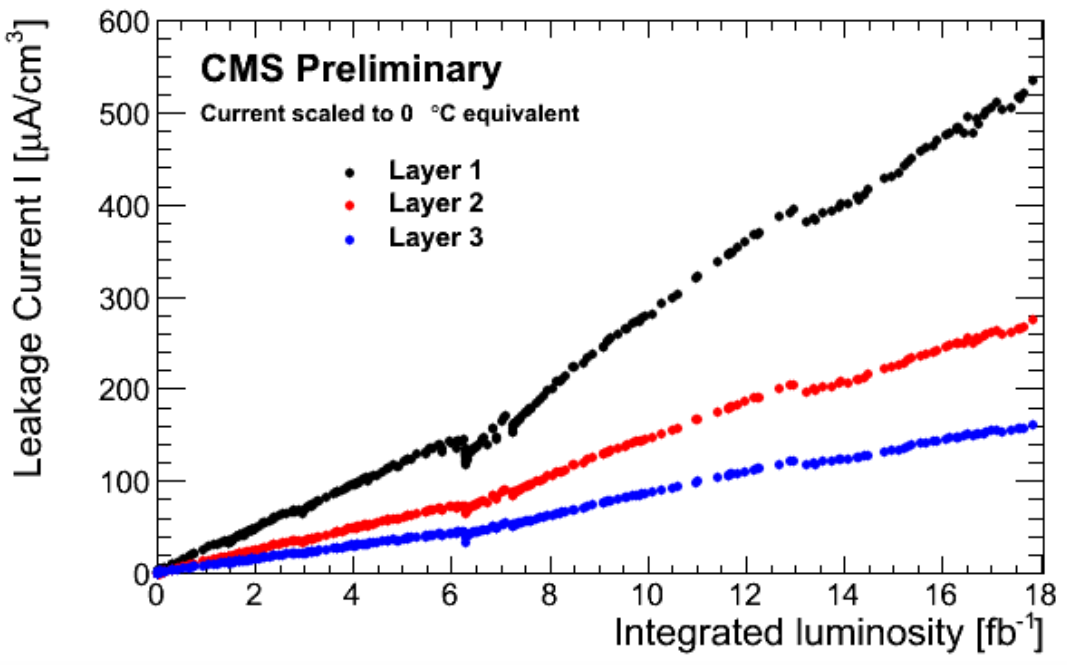
\includegraphics[width=0.45\textwidth]{\chfifteen/PixelLeakageCurrent-1.png}}
 \subfigure[]{\label{fig:PixLeakageCurrent_b}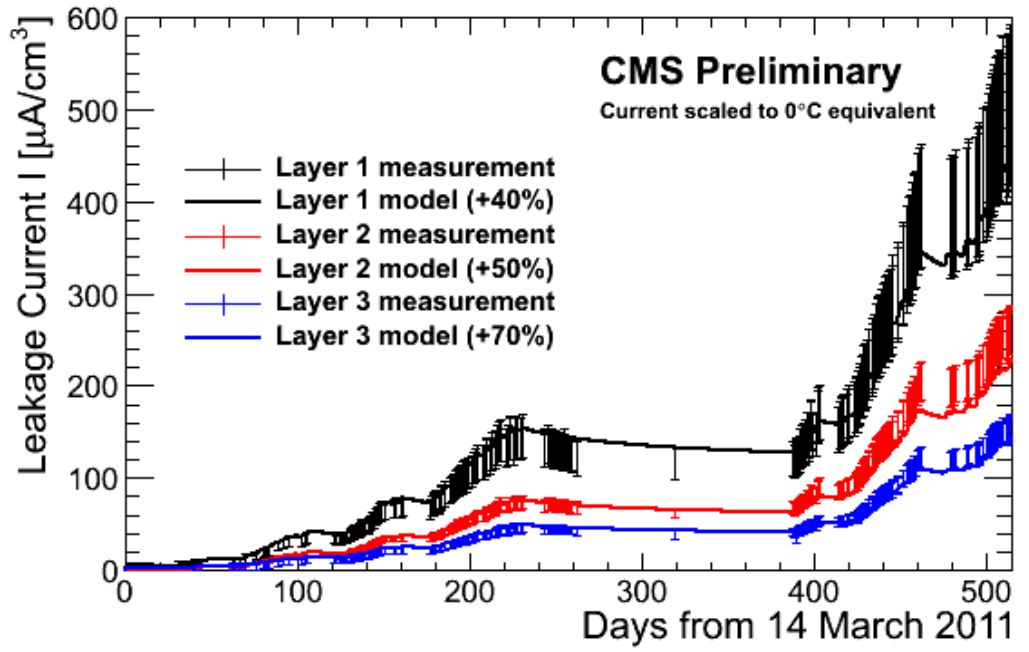
\includegraphics[width=0.43\textwidth]{\chfifteen/PixelLeakageCurrent-2.png}}
 \end{center}
 \caption{Leakage current scaled to 0\unit{$^\circ$C} operational temperature for the barrel layers as a function of the integrated luminosity (a) and time (b) in 2011-2012~\cite{Zenz:2013rva}.}
 \label{fig:PixLeakageCurrent}
\end{figure}

The depletion voltage was also monitored during operations.
With irradiation, defects with a negative space charge are generated throughout the bulk leading to variations in the effective doping concentration.
When starting with n-type bulk, the effective doping concentration decreases because of the negatively charged defects until the bulk is transformed into an effective p-type.
This process, called \textit{type inversion}, happens at a relatively low dose of several $10^{12}$\unit{$n_{eq}/cm^2$} (neutron equivalent fluence)~\cite{PixelDetectorsBook2006}.
As a consequence of this space charge sign inversion, the depletion zone now expands from the n$^+$ pixel implants towards the p-type back.
The depletion voltage scales with the bulk doping concentration: it initially decreases reaching a minimum at the inversion point, and then rises with the effective bulk doping concentration.

A dedicated scan of the bias voltage was performed several times per year, by varying the detector bias voltage from 0\unit{V} to the the normal operating value of 150\unit{V}, and measuring the single hit efficiency.
The results of the hit efficiency measurements for the innermost barrel layer between 2011 and the beginning of 2013 are shown in Fig.~\ref{fig:PixBiasV_a}.
The bias voltage that is needed to reach a depletion depth corresponding to full hit efficiency decreases with irradiation at first, then increases as expected due to the aforementioned changes in the effective doping.
The dependence of the voltage needed to achieve full hit efficiency on the integrated luminosity is shown in Fig.~\ref{fig:PixBiasV_b} for the barrel layers and endcap disks.
The presence of a minimum for the layer 1 and layer 2 is evidence for type inversion occurrence.\\

\begin{figure}[!htb]
 \begin{center}
 \subfigure[]{\label{fig:PixBiasV_a}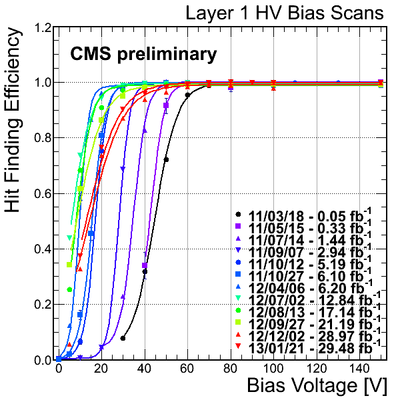
\includegraphics[width=0.3\textwidth]{\chfifteen/hv_l1_eff.png}}
 \subfigure[]{\label{fig:PixBiasV_b}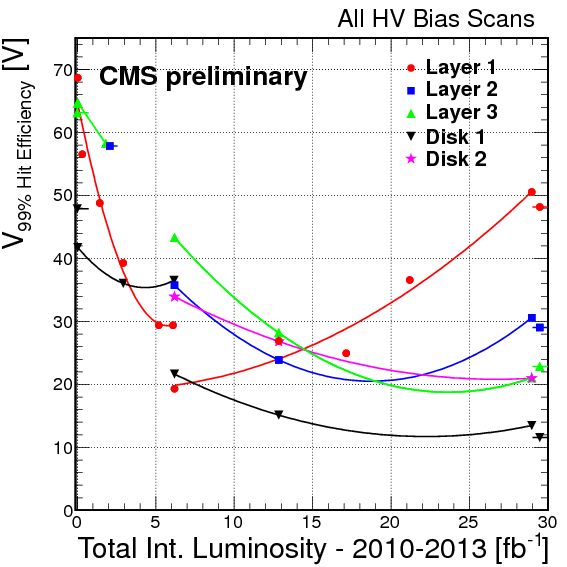
\includegraphics[width=0.3\textwidth]{\chfifteen/hvturnon_totlumi.png}}
 \end{center}
 \caption{(a) Scans of the bias voltage performed on the innermost barrel layer. (b) Bias voltage corresponding to full single hit efficiency for all barrel layers and forward disks as a function of the integrated luminosity delivered in Run~1~\cite{PixelOffline}.}
 \label{fig:PixBiasV}
\end{figure}

The evolution of the pixel threshold (Fig.~\ref{fig:PixRadDamag_a}) and the analog current (Fig.~\ref{fig:PixRadDamag_b}) was also frequently monitored in Run~1,
and an increase of both parameters with integrated luminosity was observed.
The possible explanation for these changes is the radiation damage in the bad-gap reference voltage circuit, which would shift all voltage settings inside the ROC.
Because of the described effect, a re-calibration of the analog voltage and the pixel threshold during technical stops was necessary to recover the optimal ROC performance.

The pixel hit resolution also exhibits a slow degradation with integrated luminosity as shown in Fig.~\ref{fig:PixRelvsLumi}. The two points of improvement correspond to re-calibrations of the pixel threshold.

\begin{figure}[!htb]
 \begin{center}
 \subfigure[]{\label{fig:PixRadDamag_a}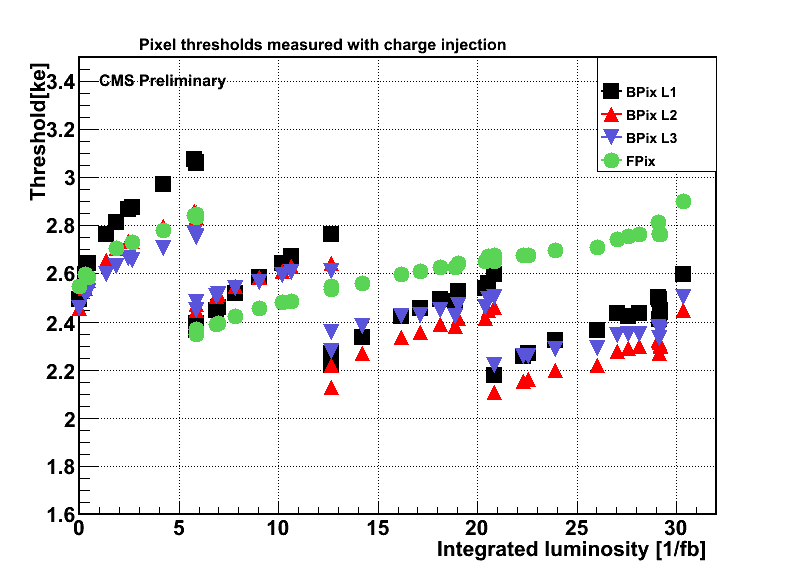
\includegraphics[width=0.45\textwidth]{\chfifteen/PixelThreshold_vs_IntLumi.png}}
 \subfigure[]{\label{fig:PixRadDamag_b}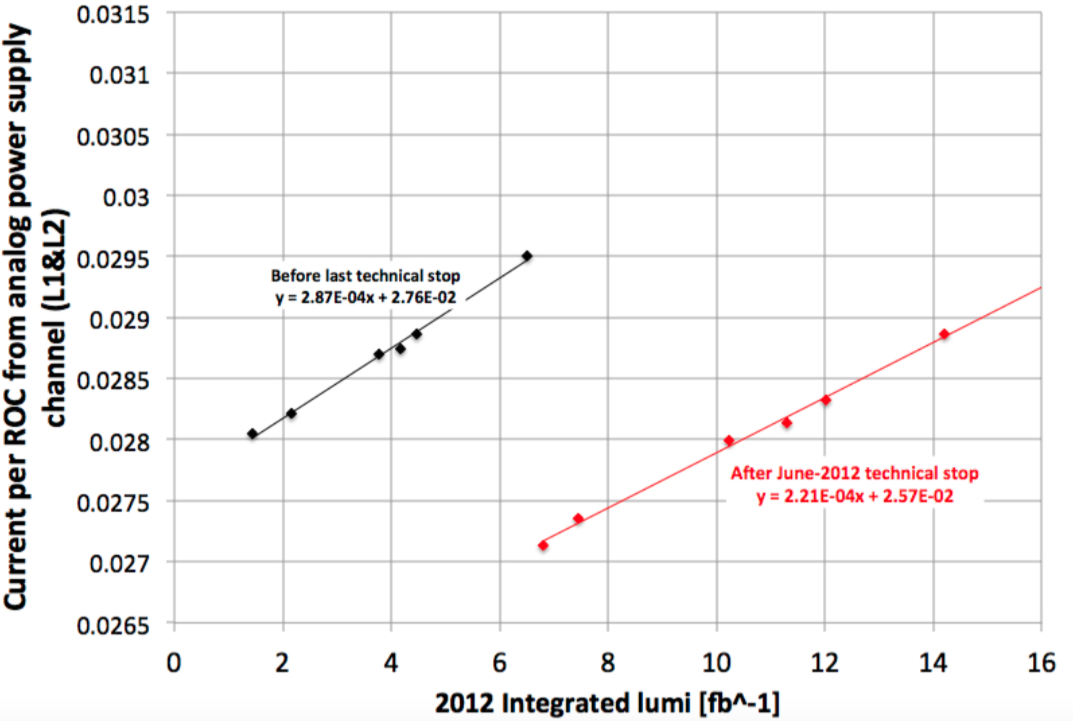
\includegraphics[width=0.45\textwidth]{\chfifteen/IanaROCvsLumi.png}}
 \end{center}
 \caption{(a) Average pixel threshold in units of 1\unit{ke} for the barrel layers and forward disks, and (b) average analog current per ROC drawn by the power supply for BPix layers 1 and 2, as a function of the integrated luminosity delivered in Run~1~\cite{PixelOffline}.}
 \label{fig:PixRadDamag}
\end{figure}

\begin{figure}[!htb]
 \begin{center}
 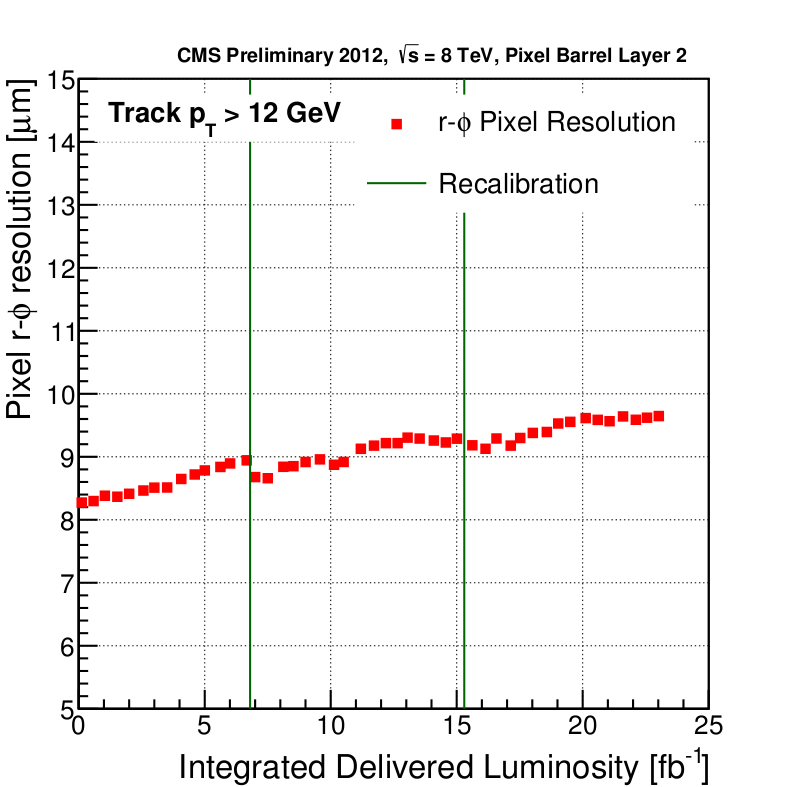
\includegraphics[width=0.45\textwidth]{\chfifteen/PixelResolutionL2_vs_IntLumi.png}
 \end{center}
 \caption{Single hit resolution for barrel layer 2 in the $r\phi$ plane as a function of the integrated luminosity delivered in Run~1~\cite{PixelOffline}.}
 \label{fig:PixRelvsLumi}
\end{figure}

%%%%%%%%%%%
\section{Optimization for LHC Run 2}
%%%%%%%%%%%

In Summer 2013, after the first LHC run, the BPix and FPix detectors were extracted from CMS, and throughout LS1 they were kept in a refrigerated, climate-controlled room environment (Fig.~\ref{fig:PixP5}) located at the CMS experimental site, LHC-P5. The BPix was maintained in two cold boxes in a laboratory with repair workbenches, and all the electronics and computers necessary to control and readout the detector for maintenance and tests.

\begin{figure}[!htb]
 \begin{center}
 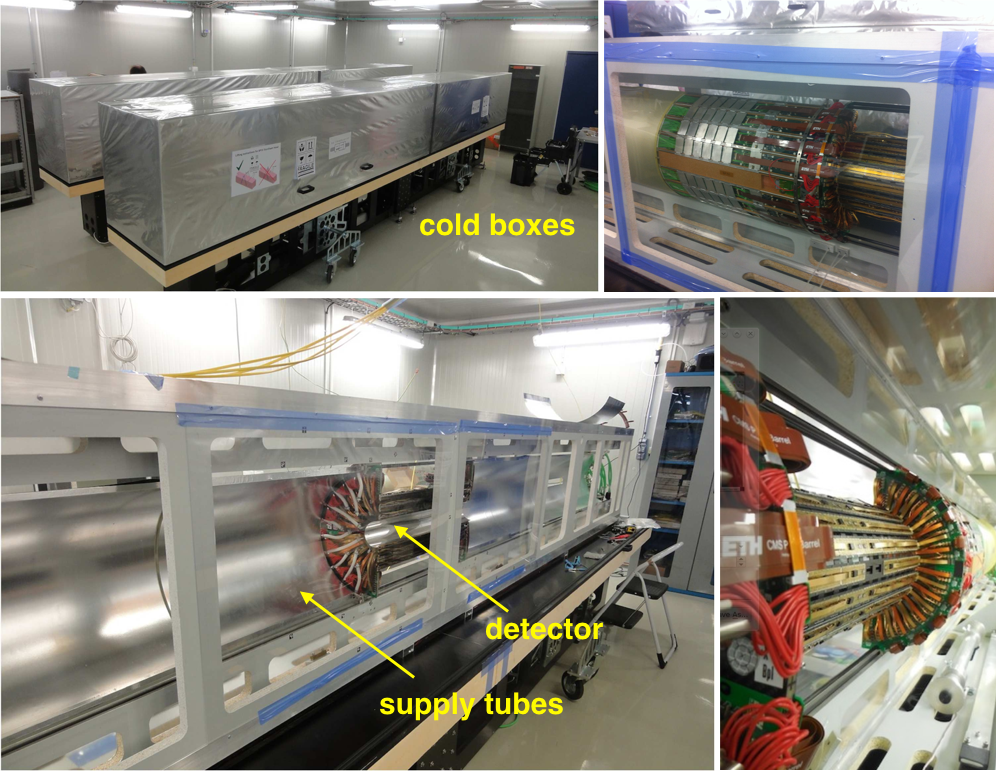
\includegraphics[width=0.7\textwidth]{\chfifteen/P5-all.png}
 \end{center}
 \caption{Barrel pixel detector temporarily installed in the clean room at LHC P5.}
 \label{fig:PixP5}
\end{figure}

At the end of Run~1, the fraction of operational channels in the barrel pixel detector was 97.7\% and the long shut-down was used to recover the faulty channels.
The main reasons were broken wire-bond connections between the ROC and the HDI as well as issues with the lasers on few AOHs.
Furthermore, some modules had an old ROC design, which caused operational problems, and were therefore disabled.
Replacements were attempted only for the barrel layer 3 outer shell, since the other layers and the inner shell of layer 3 were considered too risky to touch without breaking further parts.
The defects in layer 3 made up 52\% of the faulty channels.
Two AOHs were found with disconnected wire bonds between the laser and the AOH PCB, and they were also replaced. Figure~\ref{fig:AOHreplace} shows pictures from the laboratory in LHC-P5 during this operation.
In order to proceed with the replacement one of the two cold boxes was opened and the half shell of interest extracted using a support equipped with rails.
The shields covering the AOHs were unscrewed and all the AOHs of the sector in the outside direction had to be unplugged in order to replace the two malfunctioning ones.
Before restoring the detector in its original position inside the box, the two new AOHs were tested by checking with the oscilloscope the variations in the optical output when changing the laser bias settings with commands sent through the tkFEC. The same tests were performed for the other functioning AOHs that had to be unplugged to perform the replacement. It was found that during the operation, two additional AOHs were damaged and they had to be replaced as well.

\begin{figure}[!htb]
 \begin{center}
 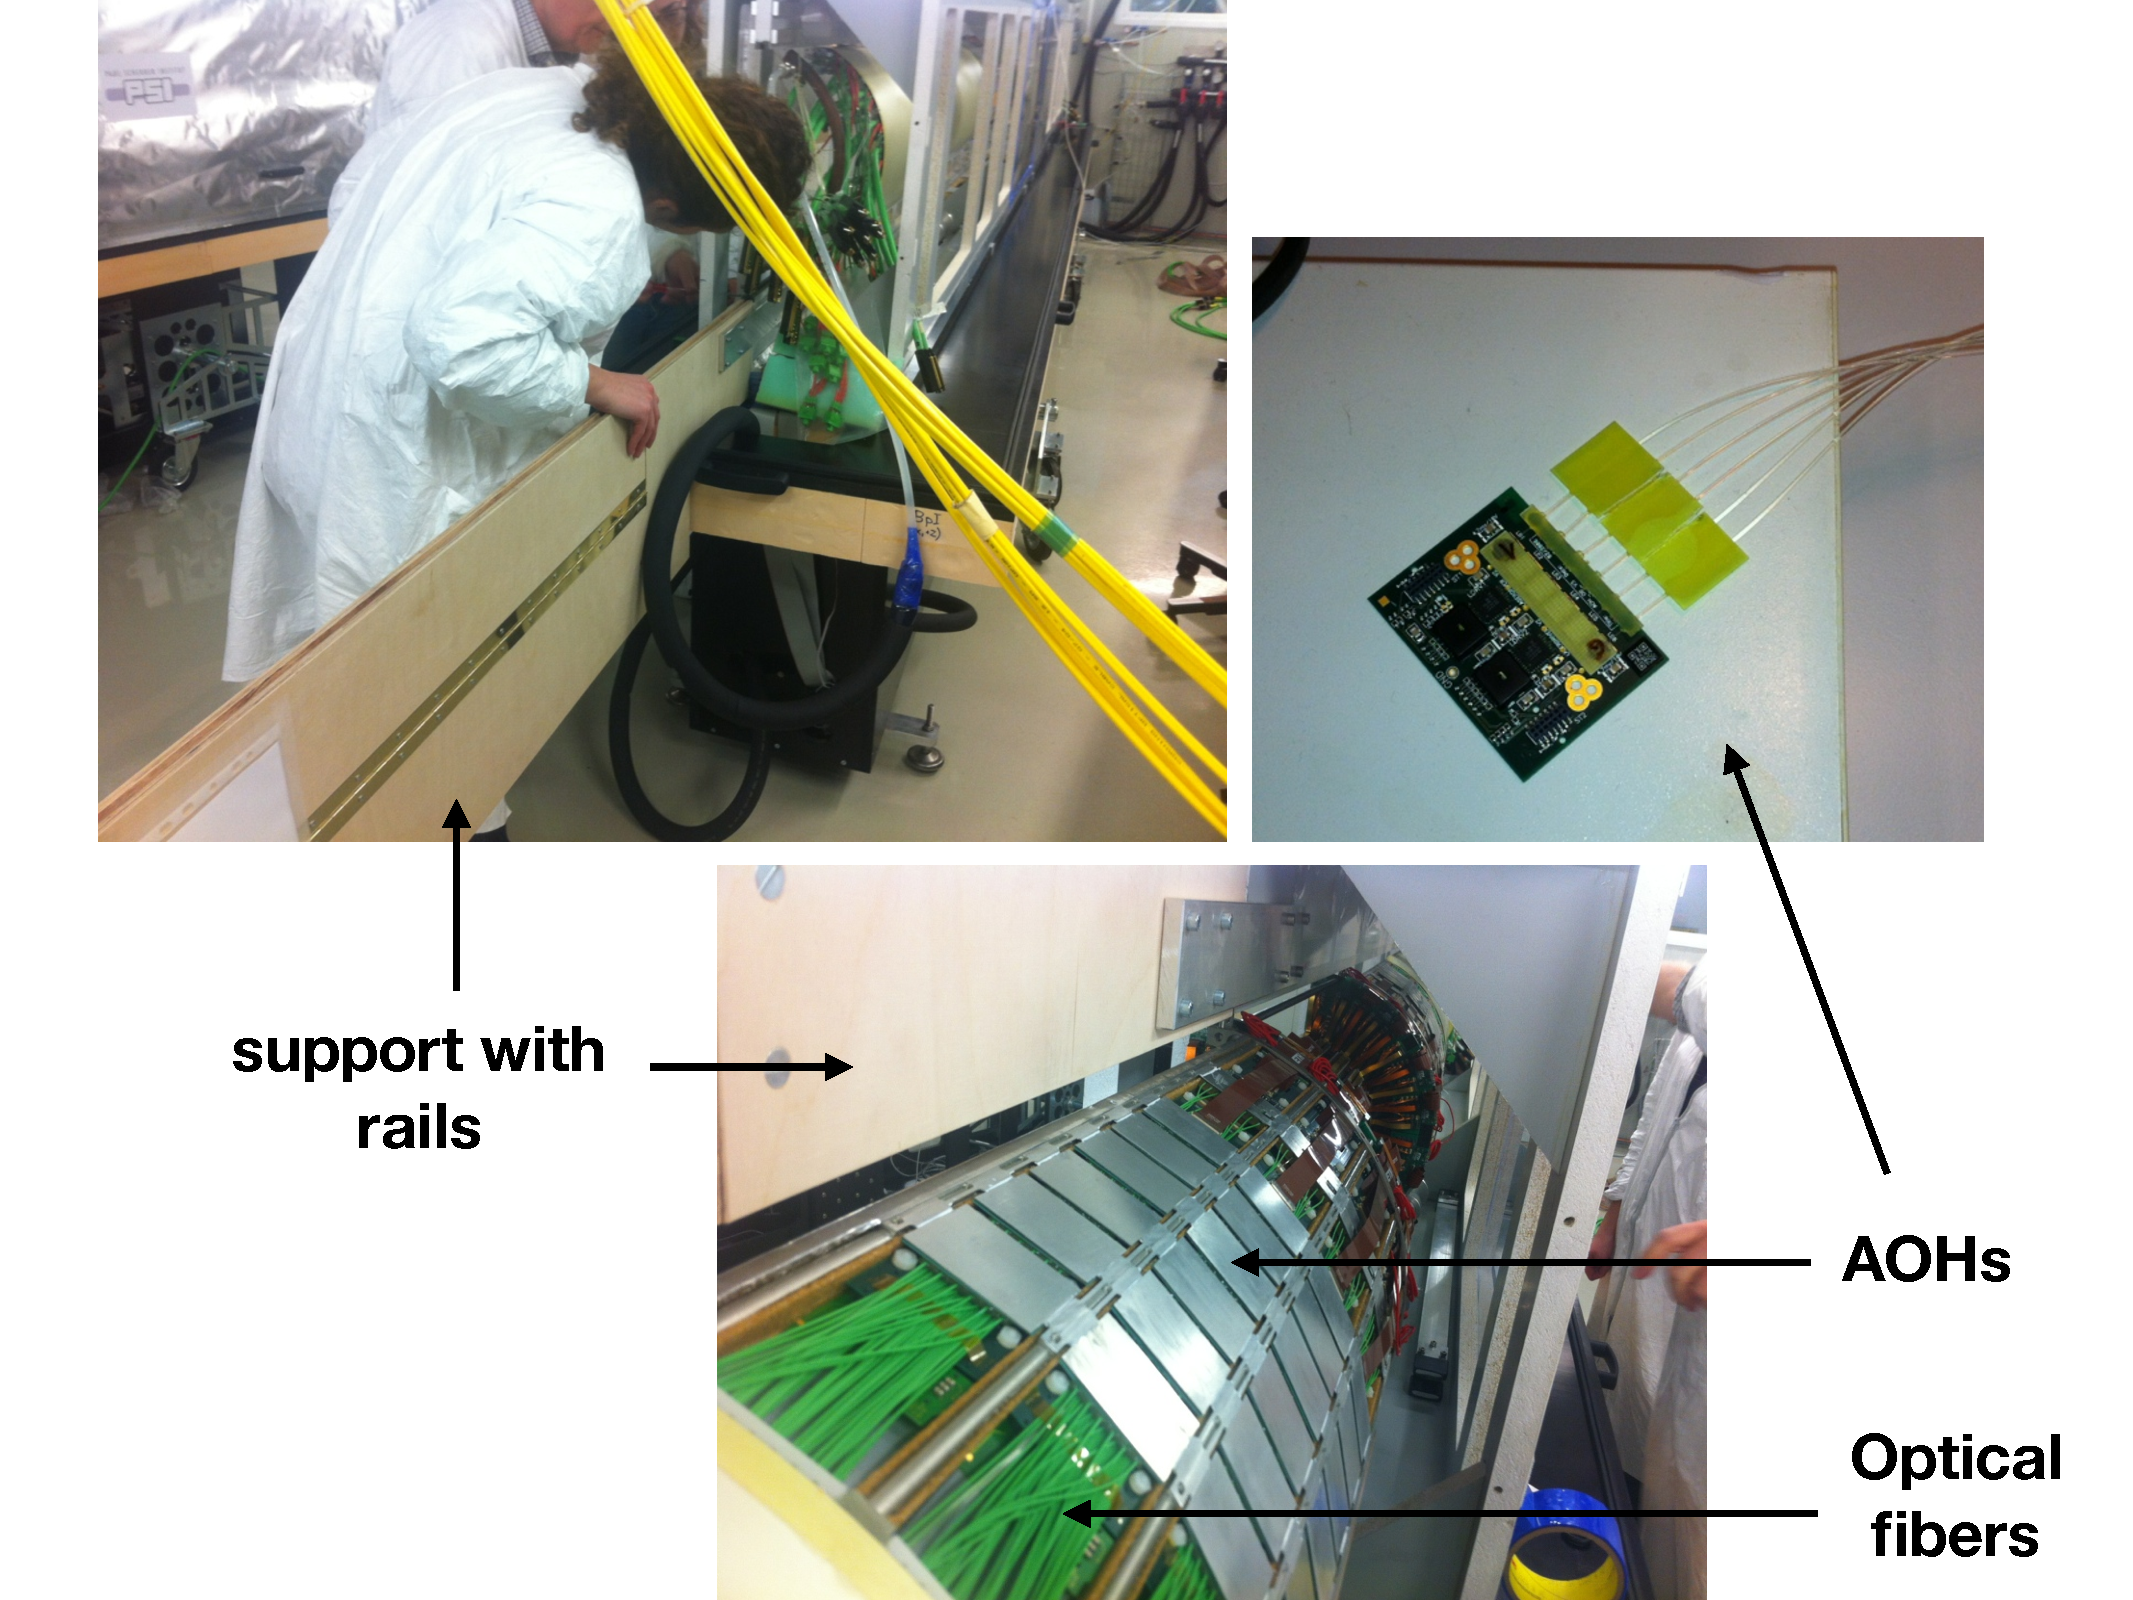
\includegraphics[width=0.7\textwidth]{\chfifteen/AOHReplacement.pdf}
 \end{center}
 \caption{Pictures of the operations conducted in the clean room at LHC-P5 to replace the broken AOHs. The support with rails used to extract one half shell from the box is visible.
 The AOHs are mounted on the supply tube and covered by metal shields. A picture of an AOH is shown on the top right.}
 \label{fig:AOHreplace}
\end{figure}

There was, however, a serious incident in mid-August 2014. After having replaced a BPix module, tests of the corresponding quadrant showed severe damage: 55 new unresponsive modules were found.
It was decided to take that part of the detector to PSI for further tests and repairs. Shorts were discovered at the ROCs and in several modules between the TBM and cable pads. Eventually, the detector was repaired within three months using 40 new modules and 19 repaired ones. The shorts were suspected to be caused by humidity due to unobserved condensation in the cold box. 
After being repaired, the functionalities of the new modules were successfully confirmed and at the end of LS1 the good detector fraction was 99\%.

Part of the time available during LS1 have been employed to exercise and improve calibration procedures in view of commissioning and operations for Run~2.
An overview of the calibration procedure is given in the following.

%%%%%%%%%%%
\section{Overview of pixel calibrations}
%%%%%%%%%%%

Detector functionality and performance depend on proper calibrations of readout chain parameters.
Most of these parameters are quite stable unless major changes occur, such as the detector operating temperature.
Other parameters are more sensitive to environmental variations.
For these parameters a re-calibration on a regular basis was necessary during Run~1 operations.

Further expertise in the calibration procedure was achieved during LS1 and it has been fundamental 
for the re-commissioning of the detector to prepare it for a successful data-taking in 2015--2016.
In addition, the detector was fully re-calibrated at low temperature after re-installation.
As for Run~1, in these two years, re-calibrations have been performed during technical stops, and in particular in mid-2016 when the analog current drawn by the ROCs of the innermost layer reached critical values ($\approx6$\unit{A}) that led to the trip of the power supplies in several occasions.

The calibrations are performed with POS which was installed and run on the computers available in the clean room.
There are a large number of different calibration tasks that need to be executed sequentially and sometimes iterated.
While a detailed description of each calibration as well as the implementation in POS can be found in Ref.~\cite{POSCalib}, an overview of the most important steps is given in the following.
The calibration process consists first of a part where the readout chain settings are adjusted. It is meant to put the detector in a state in which it can correctly reconstruct hits and involves tuning of the settings of the FED,
of the electronic components placed on the supply tubes, as well as the threshold and timing settings of the ROCs, which are controlled by programmable DACs (Section~\ref{subsec:BPix_ROC}).
In the second part of the process the pulse height information is optimized. The steps involved here are lengthy and require several iterations to reach the target signal rise speed as well as the lowest practical value for the threshold of each ROC. In the final step, an optimization of the analog signal response is performed.
Most of the calibrations produce directly new optimal settings which can then be used in subsequent runs.
Other calibrations write binary data files which have to be analyzed offline, these include the pixel alive test, the threshold and noise measurement and the gain calibration.

\subsection{Adjustment of readout chain settings}\label{subsec:calibPart1}

\subsection*{1) Delay25 chip}

As described in Section~\ref{sec:BPix_DAQ} (Fig.~\ref{fig:BPixSystem}), the LHC clock, L1 trigger and programming signals are transmitted from the pxFEC placed in the underground counting room to the detector through fibers.
The optical signals are first converted into digital signals by the DOH to be then sent to the detector through the Delay25, PLL and Gate-Keeper chips integrated in the same digital circuit.
The clock and trigger are encoded as a single signal transmitted using one single fiber.
As schematically illustrated in Fig.~\ref{fig:DigitalCircuit}, this signal is decoded by the PLL chip and sent via two separate lines, LHC clock (CLK) and Calibrate/Trigger/Reset (CTR), through the Delay25 chip to the BPix modules.
In addition, the CLK signal is split in the Gate-Keeper chip and one line (RCK) is returned and sent back to the pxFEC through the Delay25 chip.
The digital programming and control data (SDA) also goes through the Delay25 and Gate-Keeper chips.
If the gate is open the SDA is transmitted to the BPix modules which sends the acknowledge signal (RDA) back, otherwise the data packet is returned in the Gate-Keeper.

\begin{figure}[!htb]
 \begin{center}
 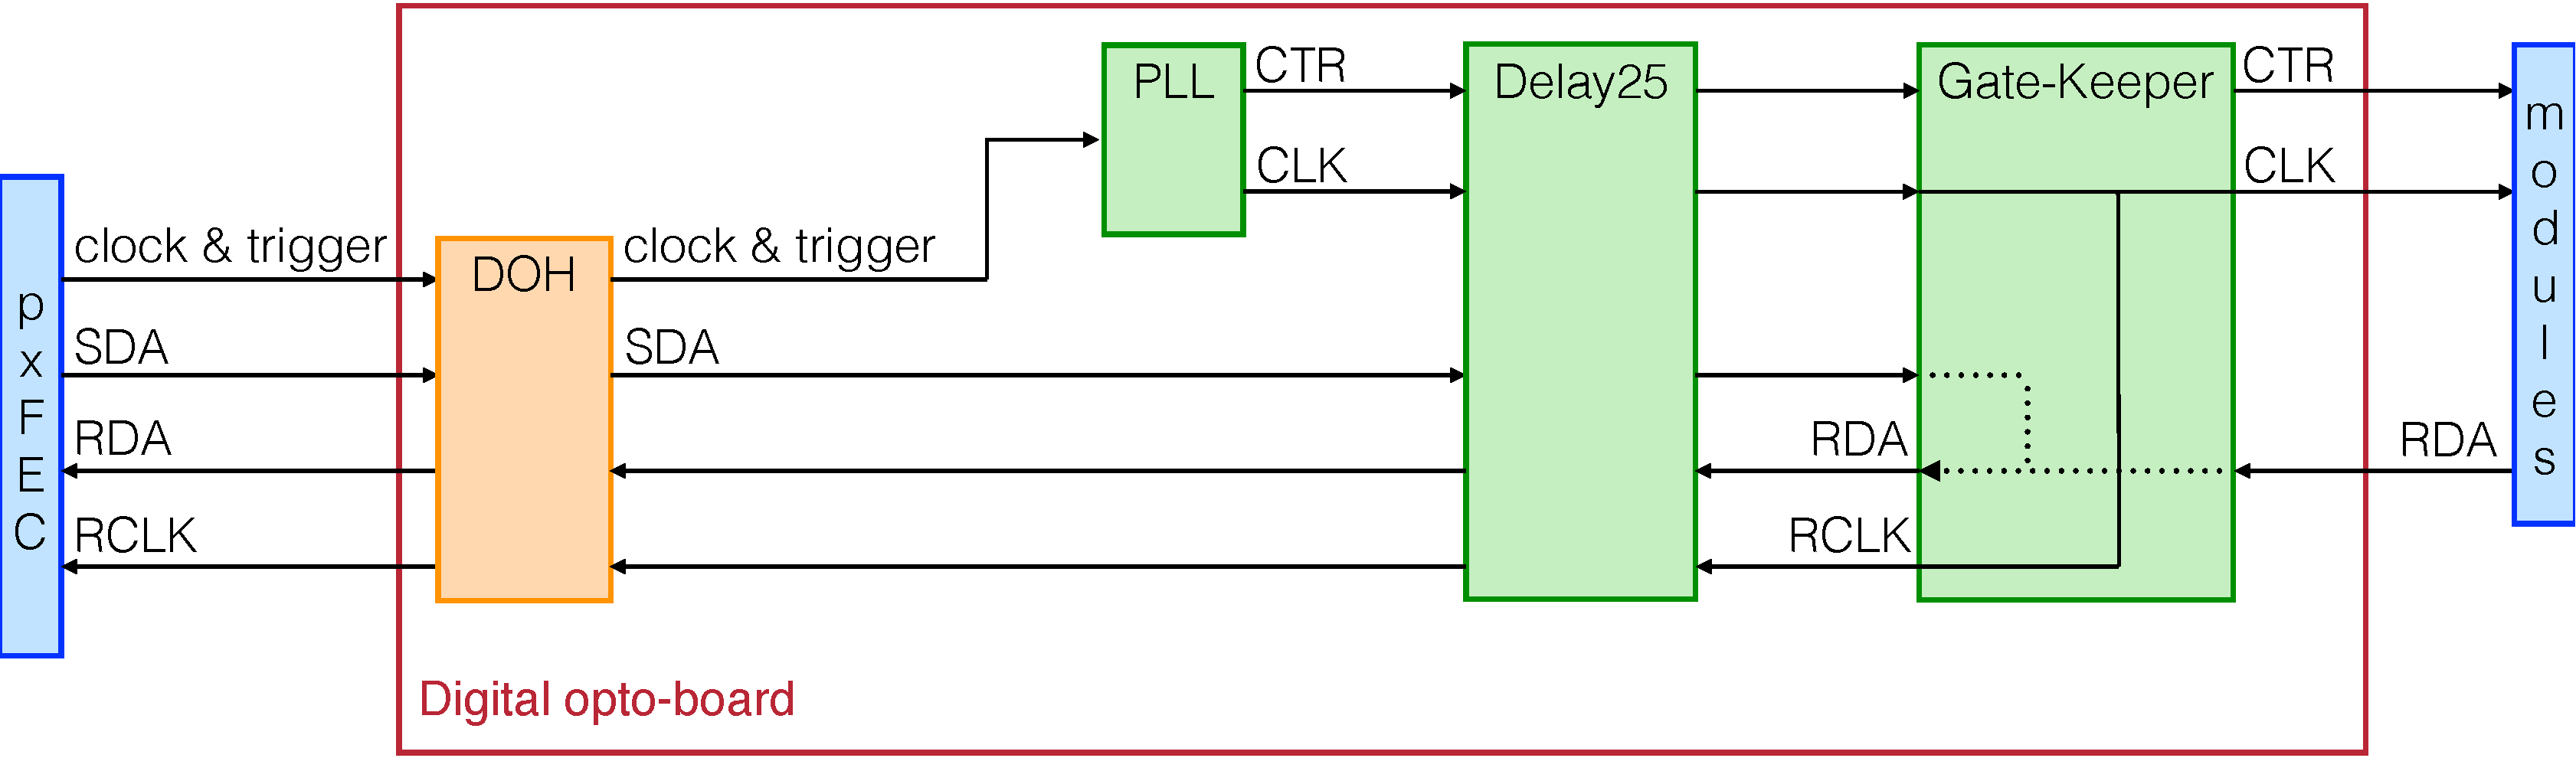
\includegraphics[width=0.97\textwidth]{\chfifteen/DigitalCircuit.pdf}
 \end{center}
 \caption{Diagram illustrating the functionality of the BPix digital circuit.}
 \label{fig:DigitalCircuit}
\end{figure}

The SDA signal can only be decoded by the TBM if it is in phase with the CLK signal. The purpose of the Delay25 chip is to adjust the timing between the two lines to make this communication work.
Hence, a calibration is performed where the delays for the SDA and RDA lines are scanned and for each set of values commands are sent to the TBM and the return status in the pxFEC is checked.
The main output from this calibration is new SDA and RDA delay settings. If the calibration converges the old settings stored in the configuration database are updated with the new ones.
An example of the scan is shown in Fig.~\ref{fig:Delay25} for one module.
The set of values chosen by the algorithm is indicated with a red point and corresponds to a region where the communication between the TBM and the pxFEC has been established for each trial.

This calibration is fundamental to ensure correct communication with the pxFEC, but once the settings are found they do not need to be readjusted often.

\begin{figure}[!htb]
 \begin{center}
 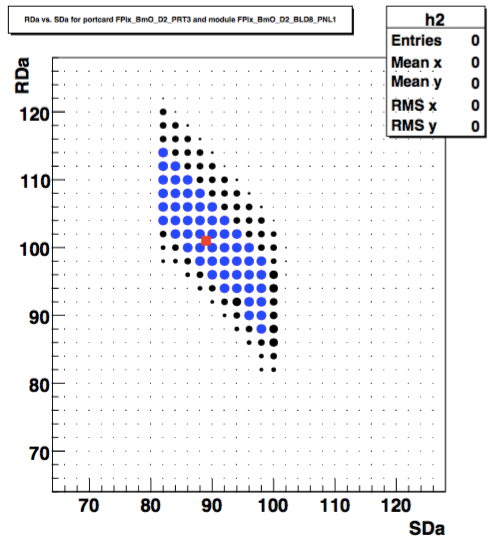
\includegraphics[width=0.45\textwidth]{\chfifteen/Delay25-2.png}
 \end{center}
 \caption{Example of output of the Delay25 calibration for one module. For each set of SDA and RDA delay settings the communication with the TBM is checked. The blue dots indicates areas with 100\% communication efficiency. The black dots indicated partial efficiency where larger dots have higher efficiency. The red square indicates the point chosen by the algorithm.}
 \label{fig:Delay25}
\end{figure}

\subsection*{2) FED receiver offset}

This calibration adjusts the individual offsets included in each input channel of the FED such that the baseline of the analog signal (black level) is tuned to be near a given target value, normally 450 ADC counts, which is near the midpoint of the dynamic range of the ADC. The main output consists of new FED parameters that, if satisfactory, are used to update the previous settings.
This calibration is performed often because the AOH is very temperature sensitive. Already 1\unit{$^\circ$C} temperature change shifts the signal by 50 ADC counts (out of 1024).
The pixel FED automatically corrects for baseline shifts during a run but it is important to start with a uniform baseline distribution.
The baseline calibration adjusts each optical input to be $\pm5$ ADC counts from the target value. During normal LHC operations it is performed at least once a day during the LHC fills.

The calibration also produces an output file with the analog signal for each module where its several components are visible, namely the TBM header and trailer, and each ROC header (Fig.~\ref{fig:FEDBaseline}).
It runs quickly and provides an information on the data buffer for each FED channel. It is therefore very useful as a debugging tool since it provides a feedback on the basic functionalities of optical links, AOHs, TBMs and ROCs, needed to assess the status of the detector.

If this step fails to converge, for instance when part of the analog signal is not visible, a calibration can be run that adjusts the timing of the signal digitization in the FED by changing the phase of the ADC clock.
This calibration is usually very stable, and needs to be repeated only when the FEDs, fibers, or other parts of the detector are touched, or if modifications of the fine phase of the global clock occur.

\begin{figure}[!htb]
 \begin{center}
 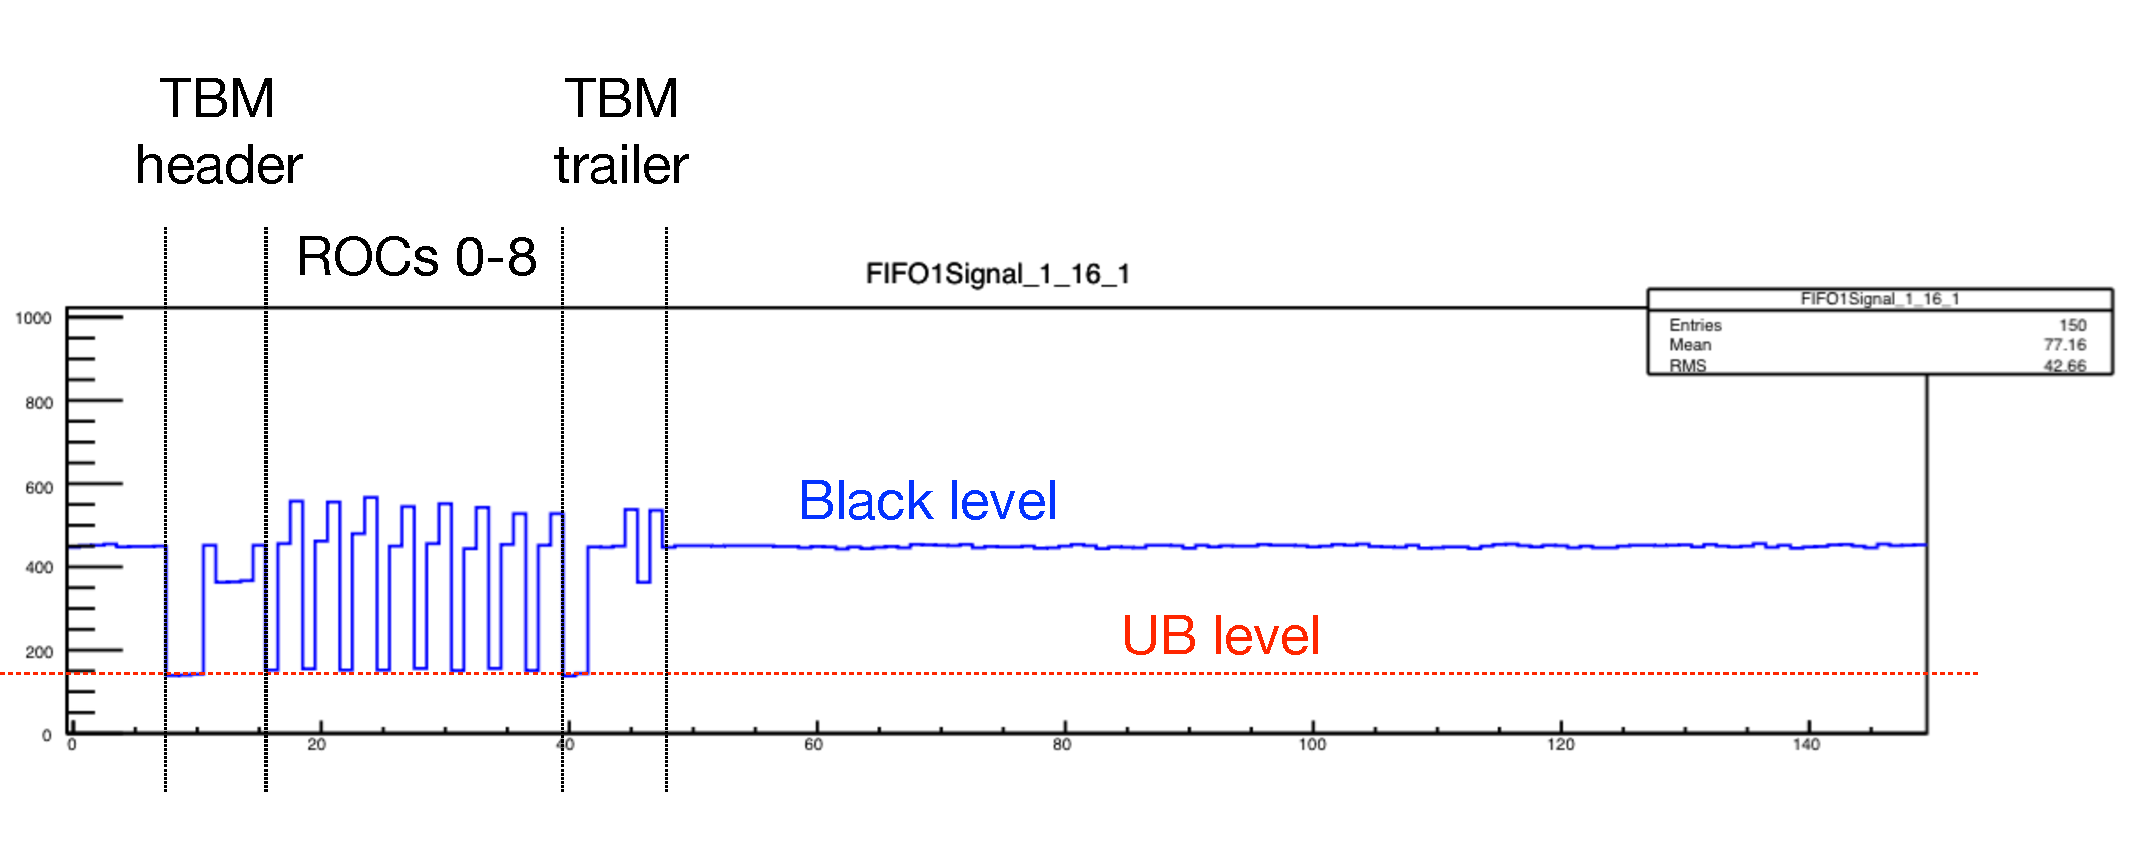
\includegraphics[width=\textwidth]{\chfifteen/FEDBaseline.pdf}
 \end{center}
 \caption{Example of analog signal from the TBM displayed at the end of the FED baseline calibration. The FED parameters are adjusted to center the baseline (or black level) in the middle of the FED ADC range.}
 \label{fig:FEDBaseline}
\end{figure}

\subsection*{3) AOH bias and gain}

Each AOH is equipped with 6 lasers for which the bias and the gain can be adjusted individually. The optical fibers connected to the lasers are combined in groups of 12 and each of them is connect to one FED channel.
The AOH bias is a setting that controls the laser bias current and hence, the amount of light (optical power) sent to the FED.
The optical power, and hence the ADC counts in the FED, increases with the laser bias setting.
As shown in Fig.~\ref{fig:AOHBias}, at low values of the bias, the black (BL) and ultra black (UBL) levels are unaffected, so that there is no separation between the two.
At some threshold, the BL begins to increase approximately linearly, followed by the UBL at a higher laser bias value and with about the same slope.

The maximum BL-UBL separation depends on the TBM settings discussed in the next section, and it is low if these parameters are configured to low values.
In fact, the BL is independent on these settings, whereas the linear rise of the UBL begins at a later point if the configured values in the TBM are higher.
As a consequence, the BL-UBL difference saturates at a higher laser bias value.
The goal of the AOH bias calibration is to determine a laser bias setting for each FED channel that is just high enough to saturate the BL-UBL difference.
The calibration measures this difference, using the levels from the TBM header and trailer, as a function of the laser bias.
It is important, though, that during this scan the TBM settings are set to reasonable values, at least as high as they will be set in later calibrations and physics runs.
Otherwise, the laser bias value determined from the saturation point will be too low.
%TBM settings above those used in this scan will not increase the B-UB separation because the AOH cannot provide more separation.

Temperature variations alter the response of the AOH, essentially shifting the curves in Fig.~\ref{fig:AOHBias} to the left or right by 4 bias counts for 5\unit{$^\circ$C} variation.
In order to provide a margin of error for these variations, the optimal laser bias setting is chosen by the calibration to be 4 counts higher than the saturation value.
This offset can be externally configured before running the calibration.

It is also important that the laser bias is not too high to avoid that the signal moves out of the dynamic range of the FED.
In the last part of the AOH bias calibration a coarse baseline adjustment is performed to bring the black level into the target range by re-adjusting the FED optical receiver offsets and laser bias settings.
%The FED channel offsets are set to the center of the range, and then the FED optical receiver offsets and AOH bias settings are adjusted to bring all FED baselines into a wide target range.
In this step the AOH bias is not decreased below the saturation value unless it is absolutely necessary.
The main output of the calibration is a new configuration for the AOH bias and FED offset values that puts all FED baselines near the center of the dynamic range, with laser bias values that allow for a large BL-UBL separation.
After the AOH bias calibration, the FED baseline calibration should be run to obtain a finer adjustment of the baseline (using the freedom to move each channel offset).

\begin{figure}[!htb]
 \begin{center}
 \includegraphics[width=0.45\textwidth]{\chfifteen/AOHBias.png}
 \end{center}
 \caption{Black and ultra black levels as a function of the AOH laser bias. An optimal value for this parameter is found at the saturation value of the BL-UBL separation.}
 \label{fig:AOHBias}
\end{figure}

The gain is a setting for each AOH laser that can accept just 4 possible values (0, 1, 2, 3).
This setting does not affect the black level, whereas it scales the size of deviations from the BL expanding or shrinking the signal.
Larger settings correspond to larger deviations and hence, to a larger BL-UBL separation.
Although the adjustment of TBM and ROC parameters will be the primary method for tuning the UBL to the optimal value, 
the aim of this calibration is to set the laser gain at the lowest level that will allow the TBM UBL to be sufficiently low for an optimal readout of the signal.
In fact, too high laser gain values will increase the power drawn and they are intended to be used to compensate for radiation damage over time.
The optimal laser gain setting is chosen as the lowest value that provides an UBL below a user-defined threshold.

\subsection*{4) TBM and ROC ultra black levels}

With the black level set at about 450 ADC counts by the FED baseline calibration and automatic correction, the next step consists in a fine adjustment of the TBM and ROC ultra black levels.
First, the TBM settings are calibrated to set the TBM header and trailer UBL to a value of about 250 ADC counts.
There are three registers on the TBM affecting the UBL, where higher configured values correspond to lower UBL and hence, larger BL-UBL separation. Furthermore, two of them affect also the signal from the ROCs.
A simultaneous scan of all three registers is usually performed.
Although higher settings generally provide lower ultra black levels, at very high values the UBL may actually increase. 
Thus, if the calibration finds multiple settings that give the target UBL, it will choose the lower ones.

Dual TBMs represent a special case. The two channels on a dual TBM share the same registers, so that they cannot be adjusted independently to tune both ultra black levels at the target value.
In this case, the settings are optimized such that one channel is at the target UBL, and the other is below.\\

A second calibration is run that sets the ultra black level for each ROC equal to the corresponding TBM's UBL.
There are two DAC settings on the ROC which affect the UBL, and higher configured values correspond to lower UBL (and larger BL-UBL separation).
%VIbias\_roc affects UB, address levels, and pulse height. VIbias\_DAC affects UB and address levels, but not pulse height. In this routine, VIbias\_DAC is scanned while VIbias\_roc is fixed.

These calibrations have to be repeated every time the previous steps 2 and 3 are run and modify the correlated parameters.

\subsection*{5) Threshold and charge injection delay}

The rest of the calibrations require the use of the charge injection feature of the ROC.
For the injected charge to be readout as a hit, it has to cross the comparator threshold and be validated by the trigger (which involves the timing of the injection).
Thus, a calibration is first run that aims at finding the settings for each ROC for the comparator threshold and for the delay at which the charge is injected into the pixels.
It is meant at quickly finding a working point in which the injected test charge can be read out.
The amplitude of the injected signal is set by programming the corresponding DAC register (\textit{Vcal}).
Since these settings are common to all pixels in a ROC, only few cells can be enabled for this calibration.
A 2D scan of the threshold and delay settings is performed: for each pair of values, a defined number of triggers are sent and for each of them the event is readout from FIFO1 or FIFO3 to verify that the hits have been collected for each ROC. The settings are changed by programming the corresponding DAC registers, \textit{VcThr} and \textit{CalDel}.

It has to be mentioned that the \textit{CalDel} setting is only relevant for calibration data taken with charge injection.
For real data, only the trigger delay has to be known and programmed into the so called \textit{WBC} register of each ROC.
The trigger delay basically sets the bunch crossing in which data is read out and is estimated from the known cable/fiber lengths and delays introduced by the electronics.

An example of \textit{VcThr} versus \textit{CalDel} scan is shown in Fig.~\ref{fig:VcThrCalDel_a}.
For large \textit{VcThr} values, which correspond to low thresholds, a large number of pixel fire due to noise such that to block a double column.
For lower values, hits are collected in the \textit{CalDel} range that corresponds to the \textit{WBC} used.
The curve bends to smaller delay values as the \textit{VcThr} decreases. The explanation for this behavior is illustrated in Fig.~\ref{fig:VcThrCalDel_b}.
Since a low \textit{VcThr} value corresponds to a higher threshold, the signal reaches the threshold later and hence a smaller delay is needed for the signal, i.e. the signal is injected earlier.

At the end of the calibration an optimal set of values is chosen in the region where the efficiency for detecting a pixel hit is 100\%.
The optimal working point is also chosen such that it is sufficiently far away from the noise level.

\begin{figure}[!htb]
 \begin{center}
 \subfigure[]{\label{fig:VcThrCalDel_a}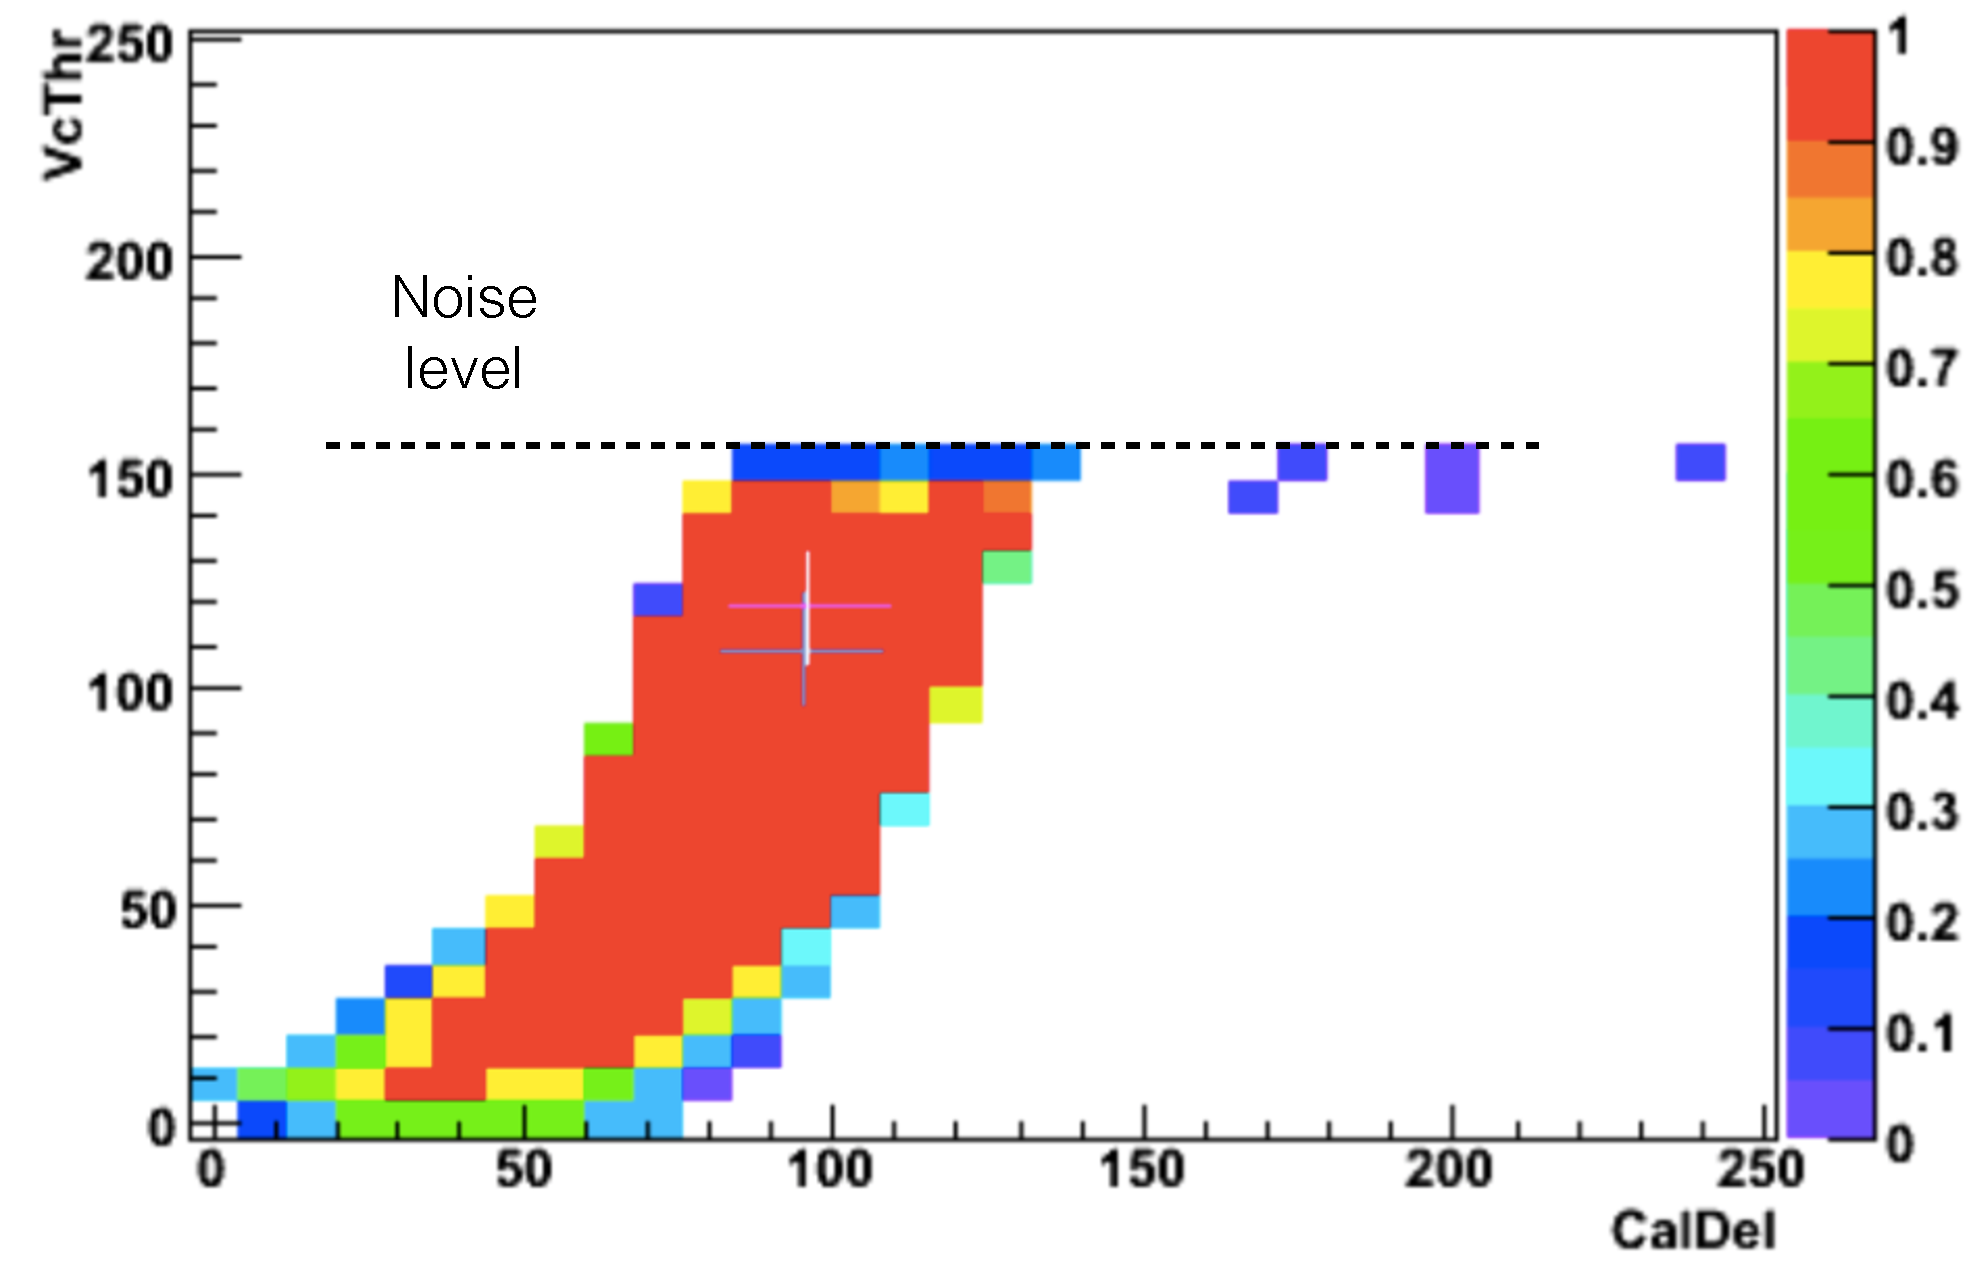
\includegraphics[width=0.5\textwidth]{\chfifteen/VcThrCalDel.pdf}}
 \subfigure[]{\label{fig:VcThrCalDel_b}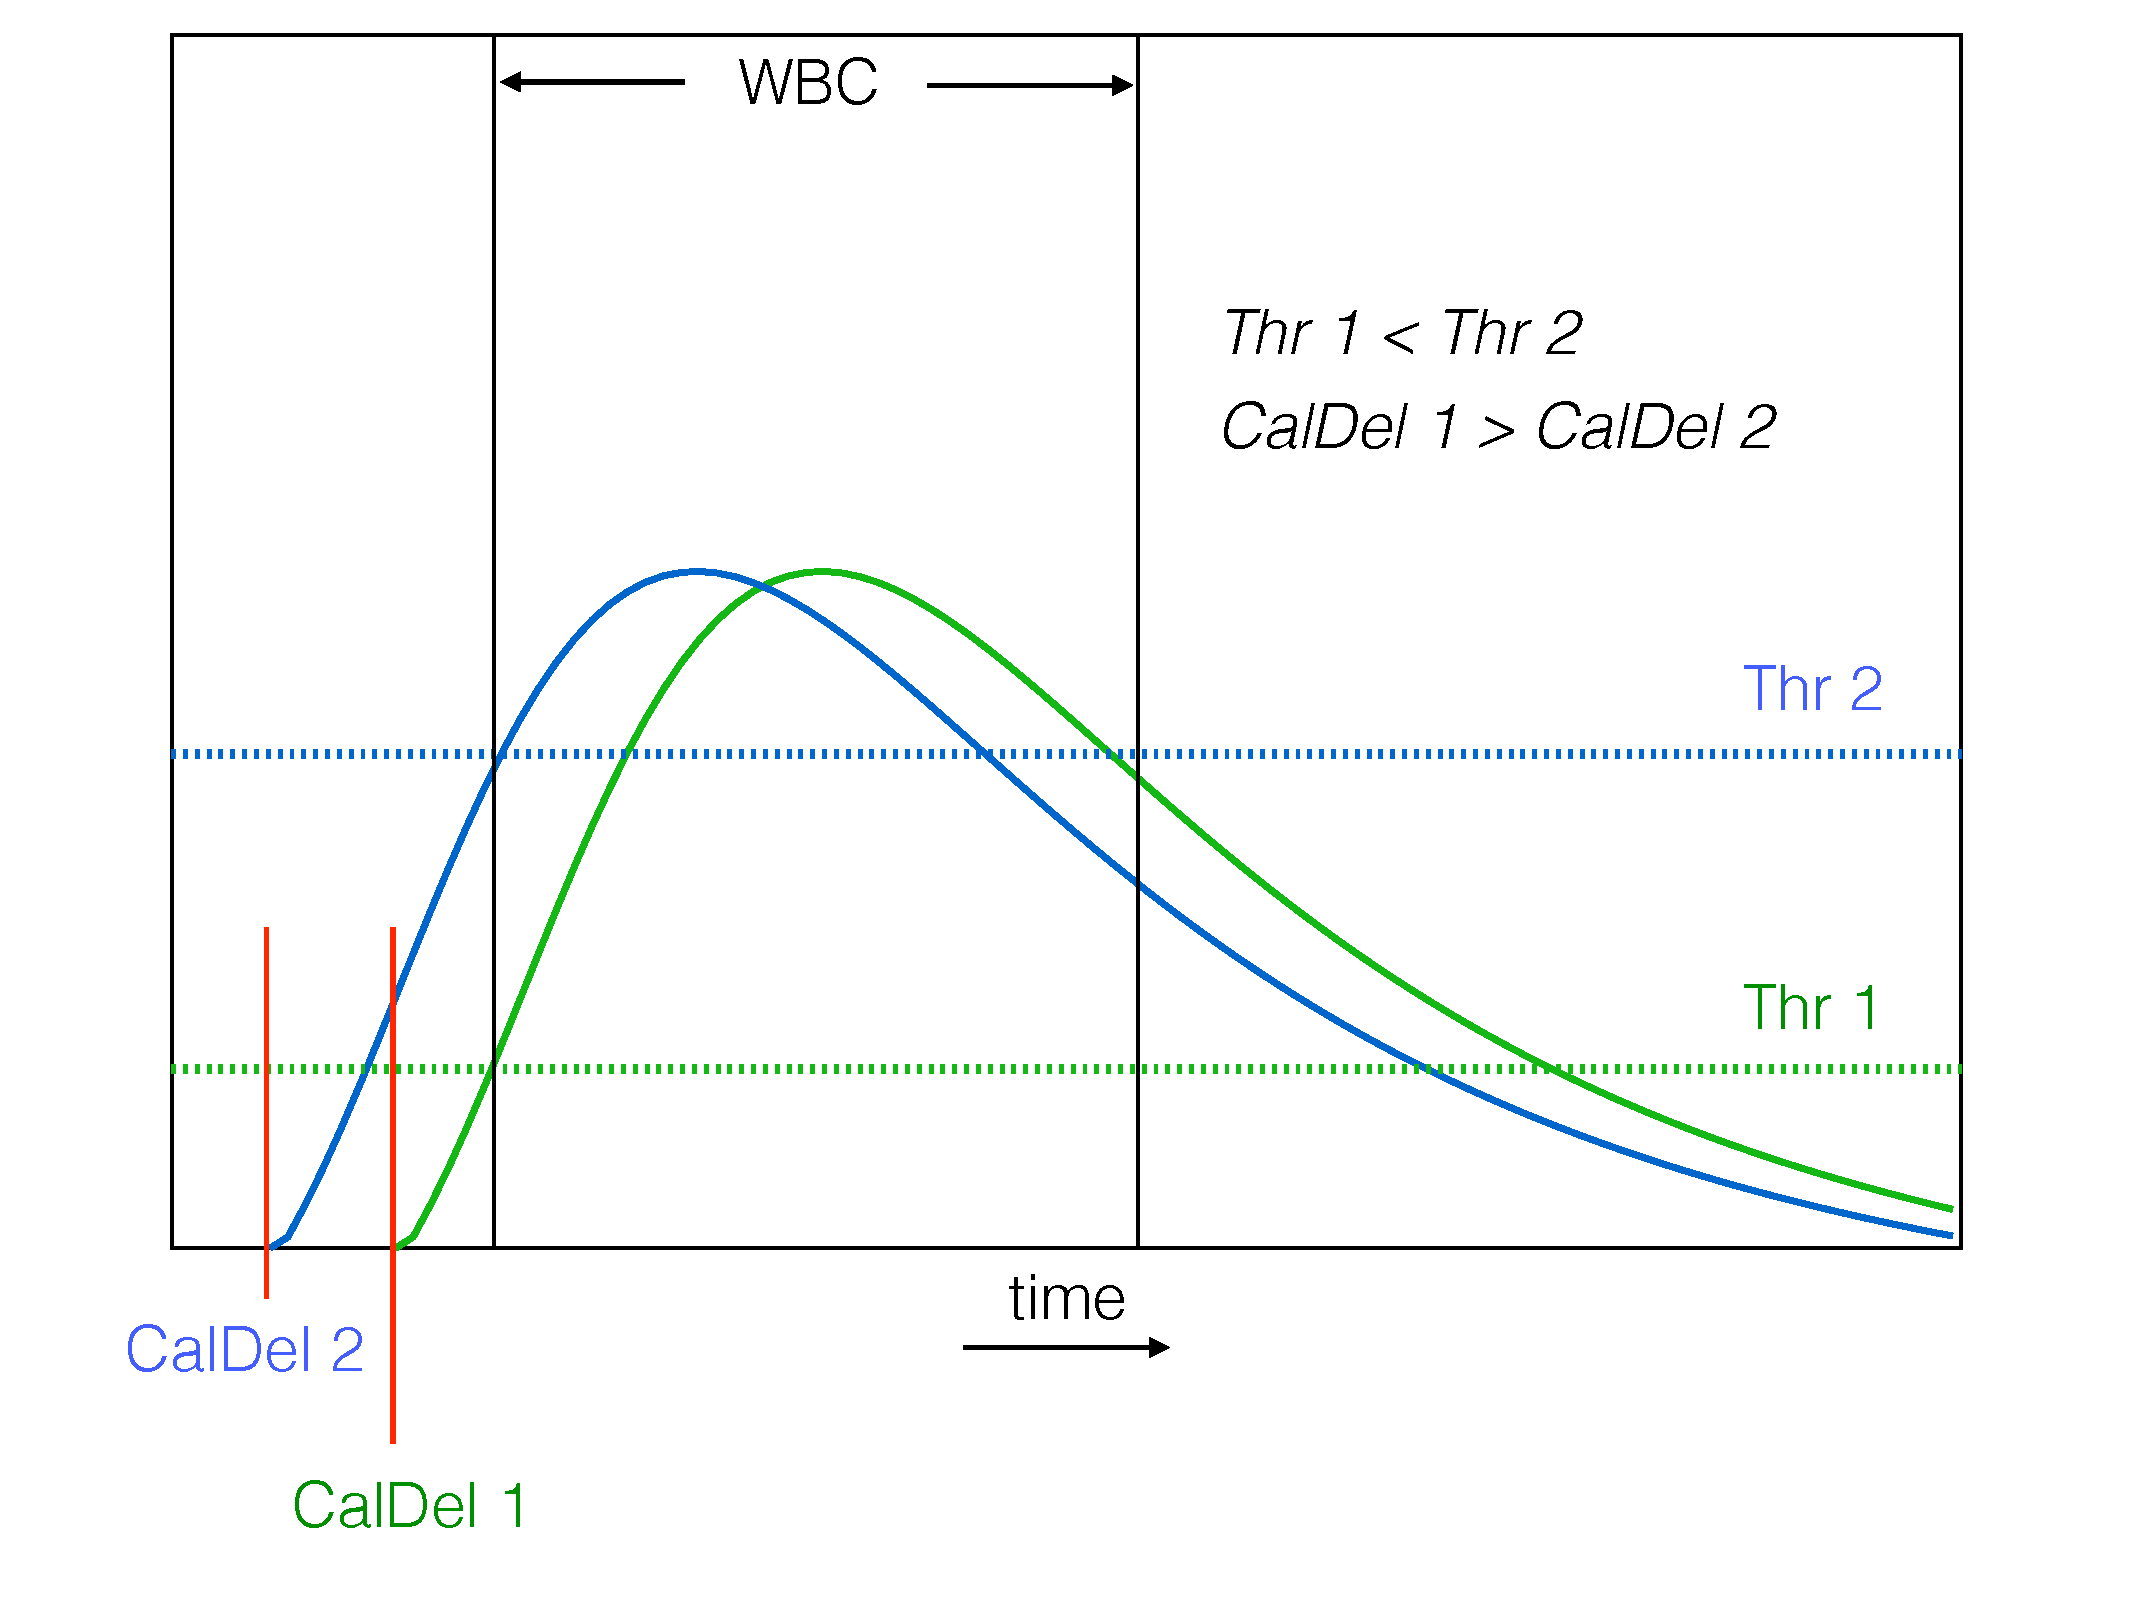
\includegraphics[width=0.4\textwidth]{\chfifteen/VcThrCalDelPulses.pdf}}
 \end{center}
 \caption{(a) Efficiency for detecting a hit as a function of the comparator threshold (\textit{VcThr}) and delay (\textit{CalDel}) settings for one ROC. Large values of \textit{VcThr}, corresponding to a low threshold, generate much noise that saturates the digital circuit and no hits are detected. The optimal point is indicated in black while the blue point indicates the old settings. For small values of \textit{VcThr} the signal reaches the threshold later and hence a smaller delay is needed for the signal. This behavior is illustrated in (b).}
 \label{fig:VcThrCalDel}
\end{figure}

\subsection*{6) Address levels}

The row and column address of the hit pixel is encoded in 6 discrete analog levels (Section~\ref{subsec:BPixReadout}) which have to be well separated for being correctly decoded by the FED.
The position of the address levels is determined by measuring the levels of all pixels in a ROC and overlaying them in a histogram.
Pixels are scanned to make sure that combinations of address levels that could potentially cause problems are probed, such as transitions from high to low levels and vice versa.
An example of the results is shown in Fig.~\ref{fig:AddressLevel}, where the six peaks corresponding to the six address levels can be seen.
The separation between the levels is good and the decoding limits are chosen in the center between to neighboring peaks to be then downloaded to the FED.
The separation can mainly be affected by dirty optical connectors and poor light transmission, or by large temperature changes not compensated by the automatic baseline correction. Hence, during stable running conditions this calibration is run once every few days.

\begin{figure}[!htb]
 \begin{center}
 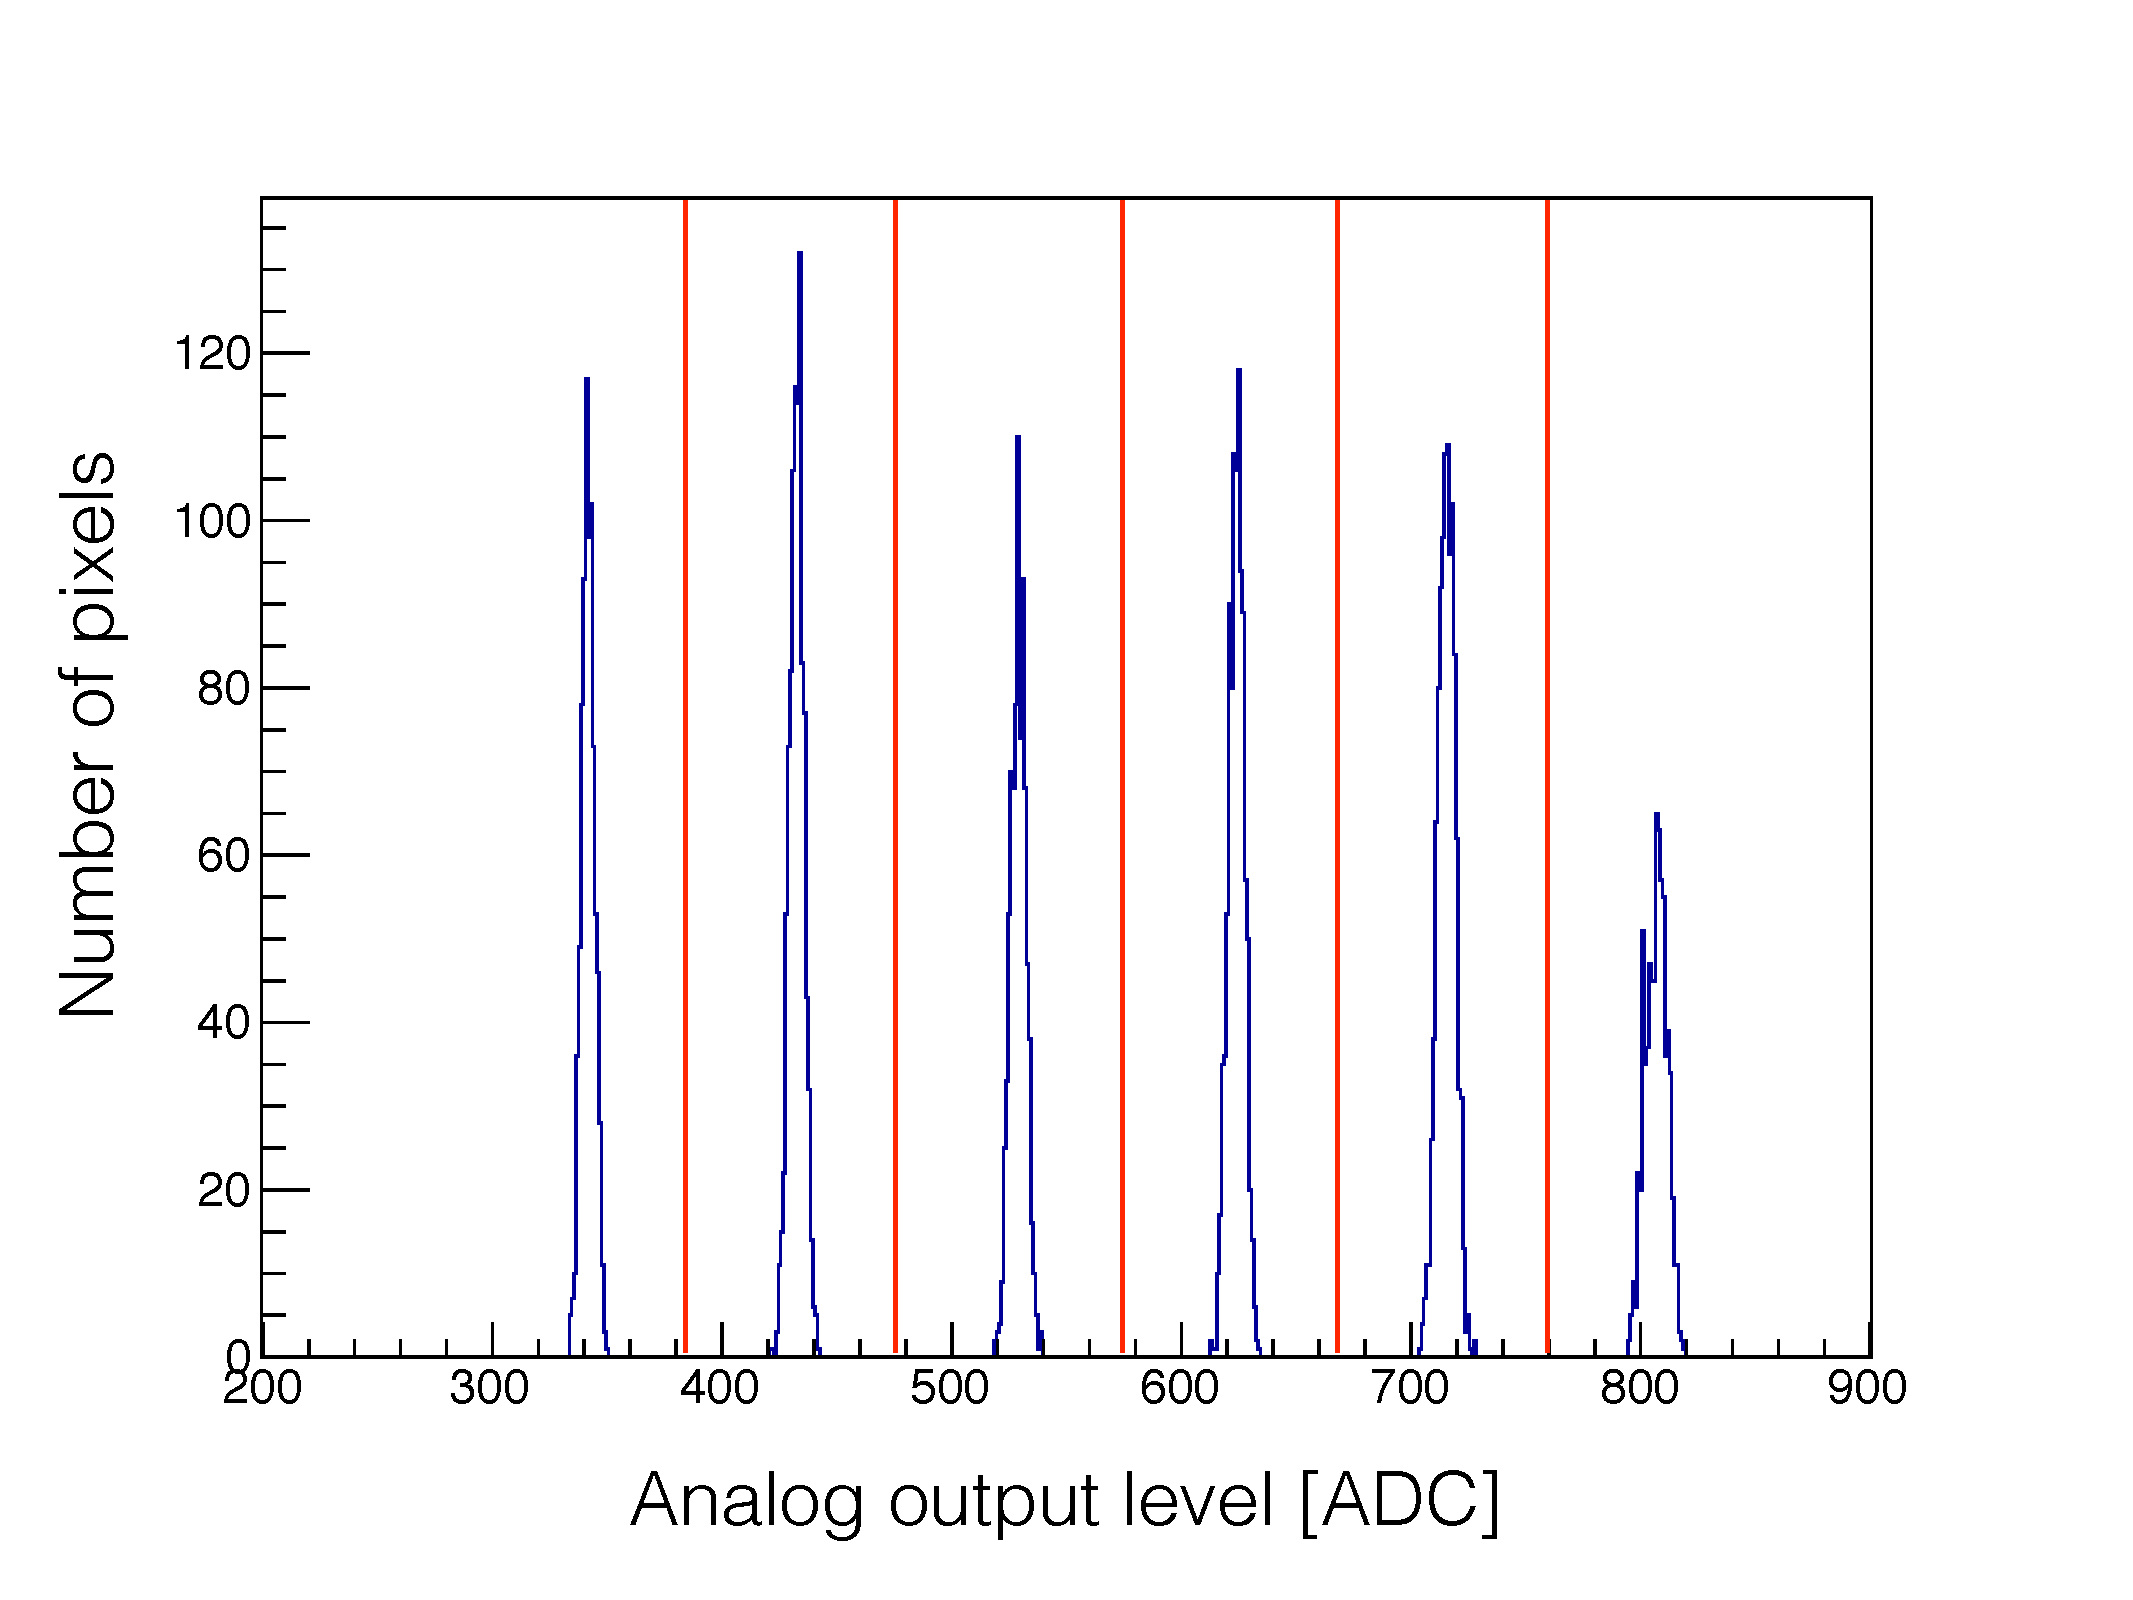
\includegraphics[width=0.45\textwidth]{\chfifteen/AddressLevel.pdf}
 \end{center}
 \caption{Address levels of all pixels in a ROC as received by the FED. The red lines are the separation limits used for the decoding of the pixel addresses in the FED.}
 \label{fig:AddressLevel}
\end{figure}

\subsection*{7) Pixel alive test}

%In this test, charges above threshold are injected into all pixels in a ROC and the correct response of each pixel is verified.
In this test, the functionality of each pixel in a ROC is checked by verifying that it responds to an injected calibration signal above threshold.
Charge is injected in each pixel several times and the number of output signals is recorded.
The pixel is fully working if all signals are registered; the pixel is defective, if no output signal is registered at all.
The data are then analyzed offline to produce an efficiency map that displays the efficiency for each pixel. Examples of the results for two ROCs are shown in Fig.~\ref{fig:PixelAlive}.
For the case on the left all cells are functioning, whereas on the right an example is shown of a ROC with a large number faulty pixels.

\begin{figure}[!htb]
 \begin{center}
 \subfigure[]{\label{fig:PixelAlive_a}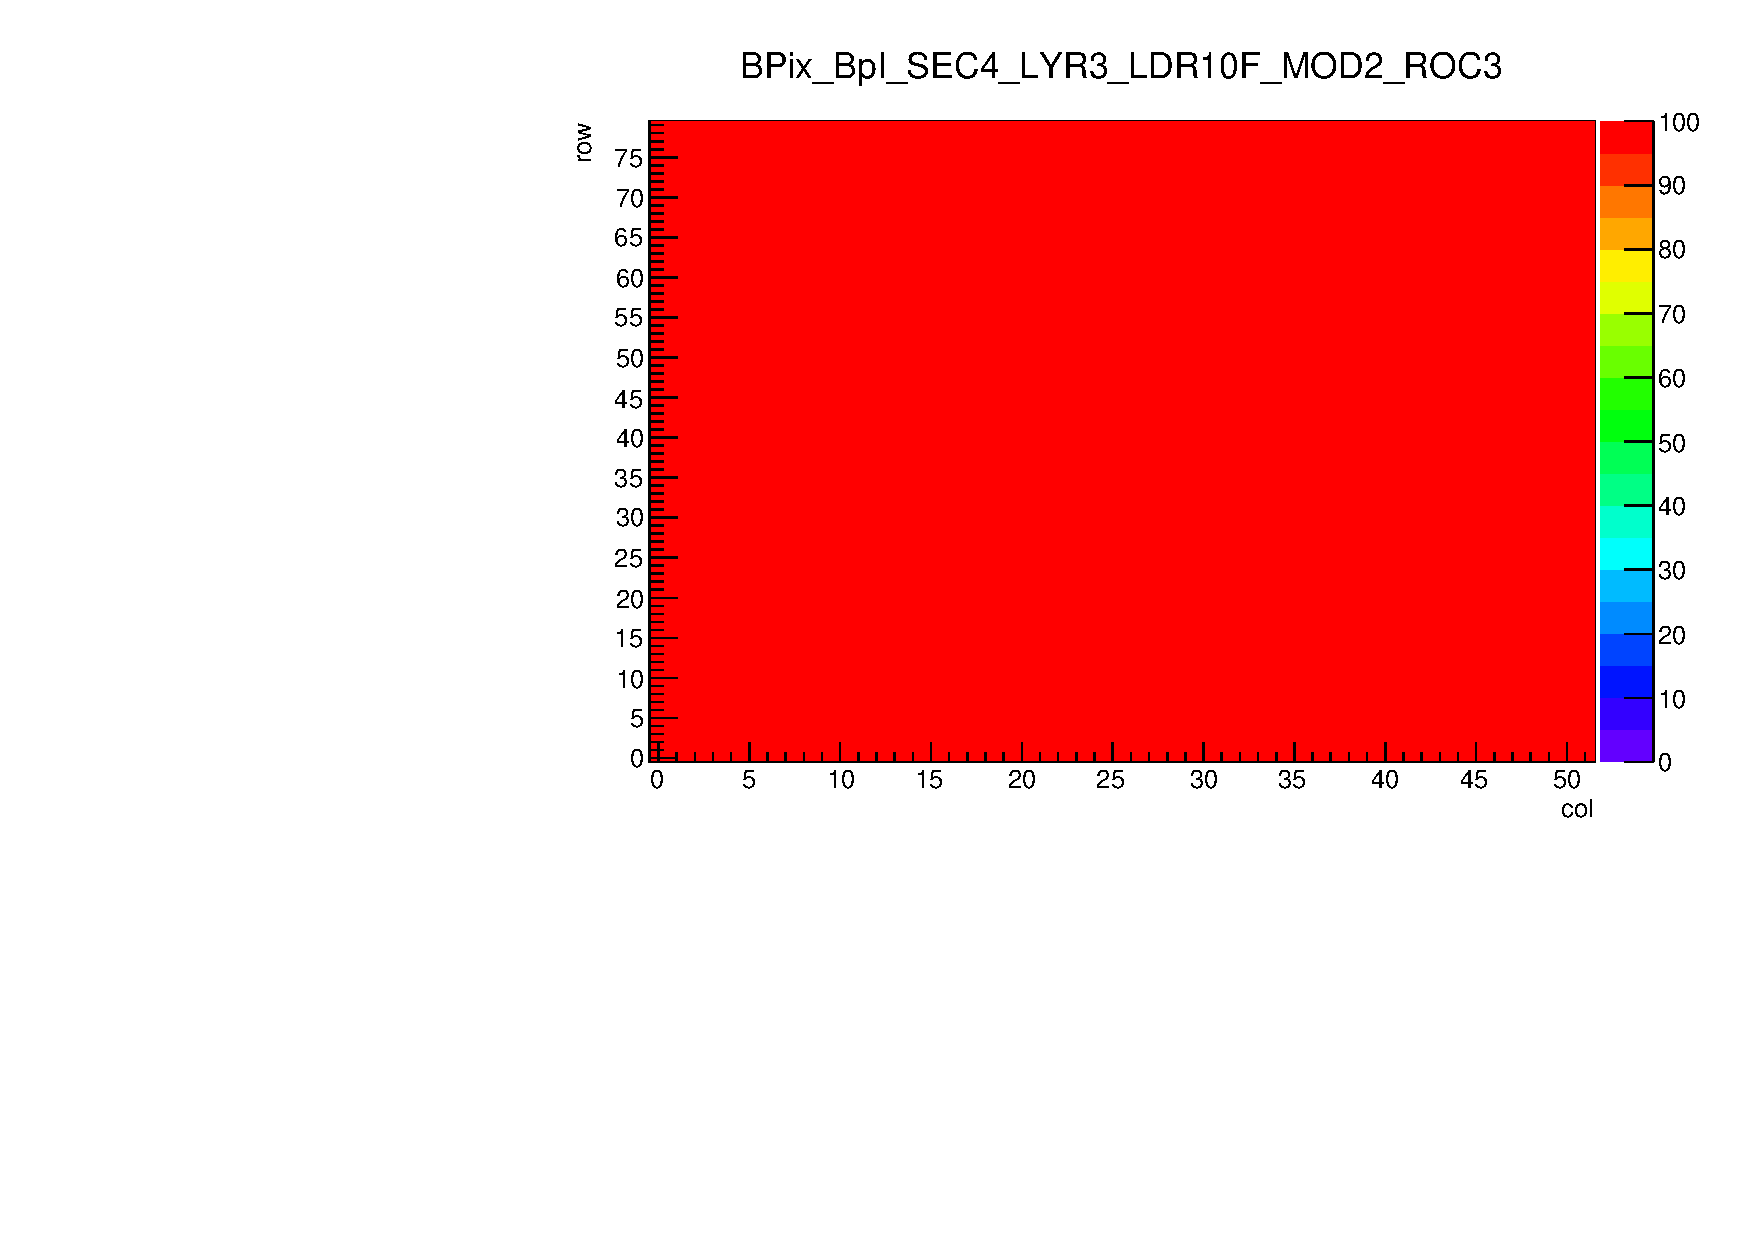
\includegraphics[width=0.45\textwidth]{\chfifteen/GoodPixelAlive.pdf}}
 \subfigure[]{\label{fig:PixelAlive_b}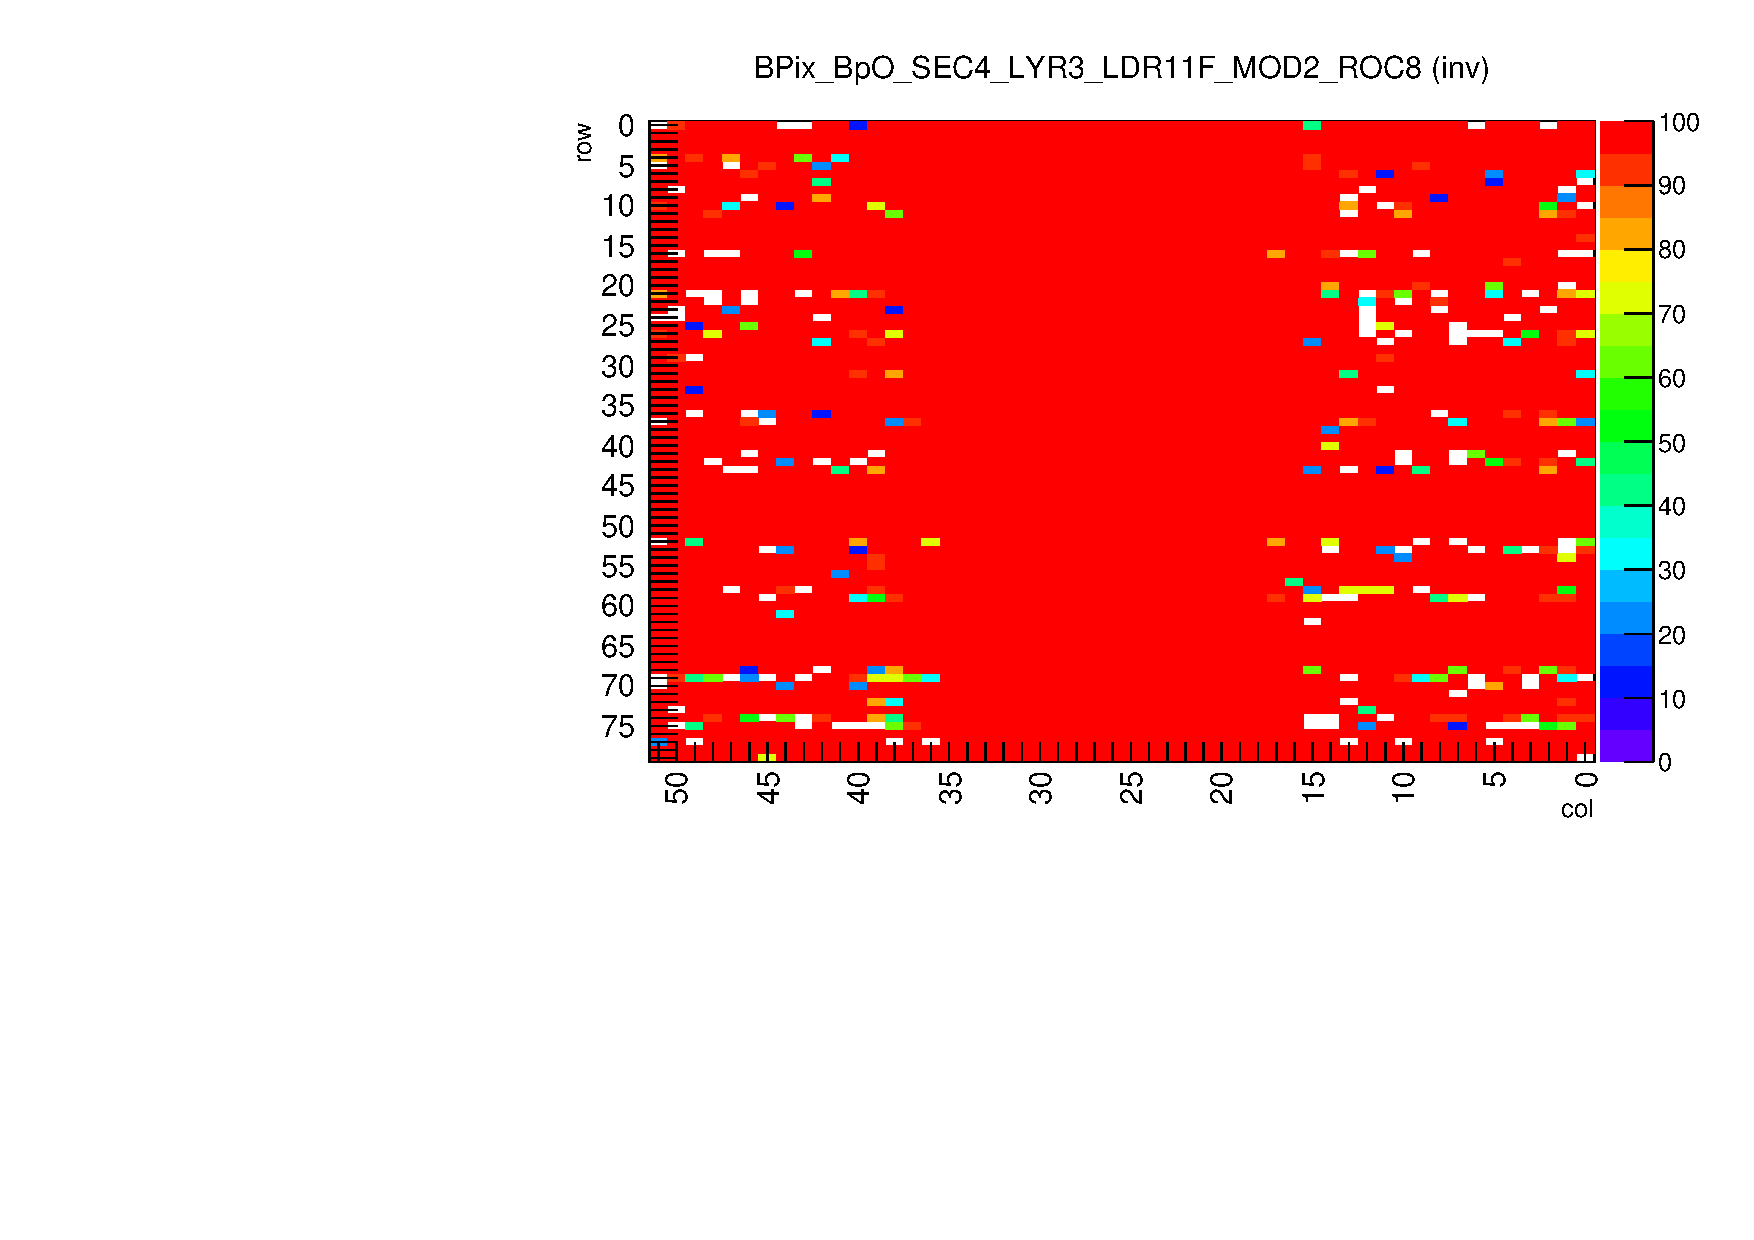
\includegraphics[width=0.45\textwidth]{\chfifteen/BadPixelAlive.pdf}}
 \end{center}
 \caption{Examples of pixel alive test results for two ROCs: (a) all cells are functioning and (b) a large number of pixels are broken.}
 \label{fig:PixelAlive}
\end{figure}

\subsection*{8) Measurement of threshold and noise}

This is the last step of the calibration chain aimed at verifying and adjusting the basic functionality of the detector.
At this stage it is important to perform a measurement of the threshold and noise of each pixel, which will be afterwards optimized in the second part of the procedure as described in the next section.
In fact, the detection thresholds are an important parameter of the pixel detector since they influence the hit position resolution (Fig.~\ref{fig:PixRelvsLumi}).

The thresholds are measured through the so called ``S-curve'' scan, which provides the pixel response efficiency as a function of the amplitude of the injected test charge (\textit{Vcal}), varied from 0 to its maximum.
The \textit{Vcal} value where the signal shows 50\% efficiency is defined as the threshold.
As for the pixel alive test, the data are analyzed offline to produce the final results.
An example of such scan is shown in Fig.~\ref{fig:SCurve_a} for a test conducted in the clean room at a temperature of -15\unit{$^\circ$C}.\\

\begin{figure}[!t]
 \begin{center}
 \subfigure[]{\label{fig:SCurve_a}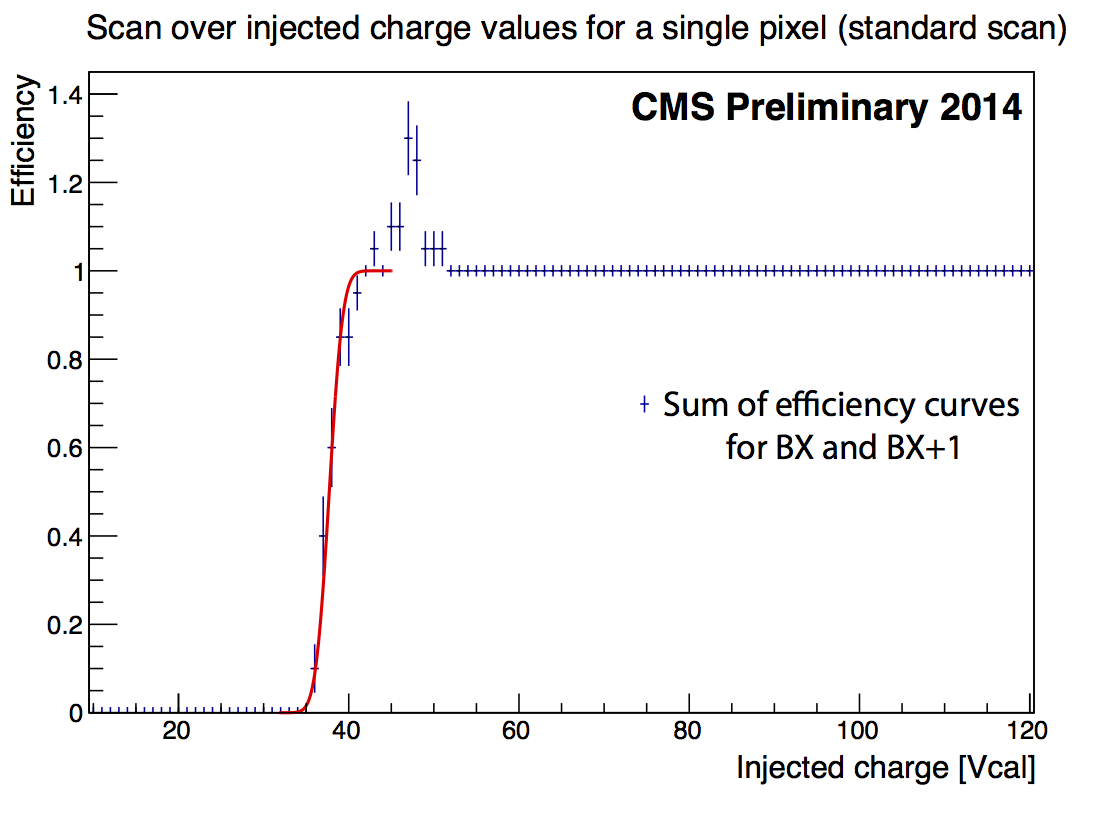
\includegraphics[width=0.45\textwidth]{\chfifteen/SCurveStandardScan.png}}
 \subfigure[]{\label{fig:SCurve_b}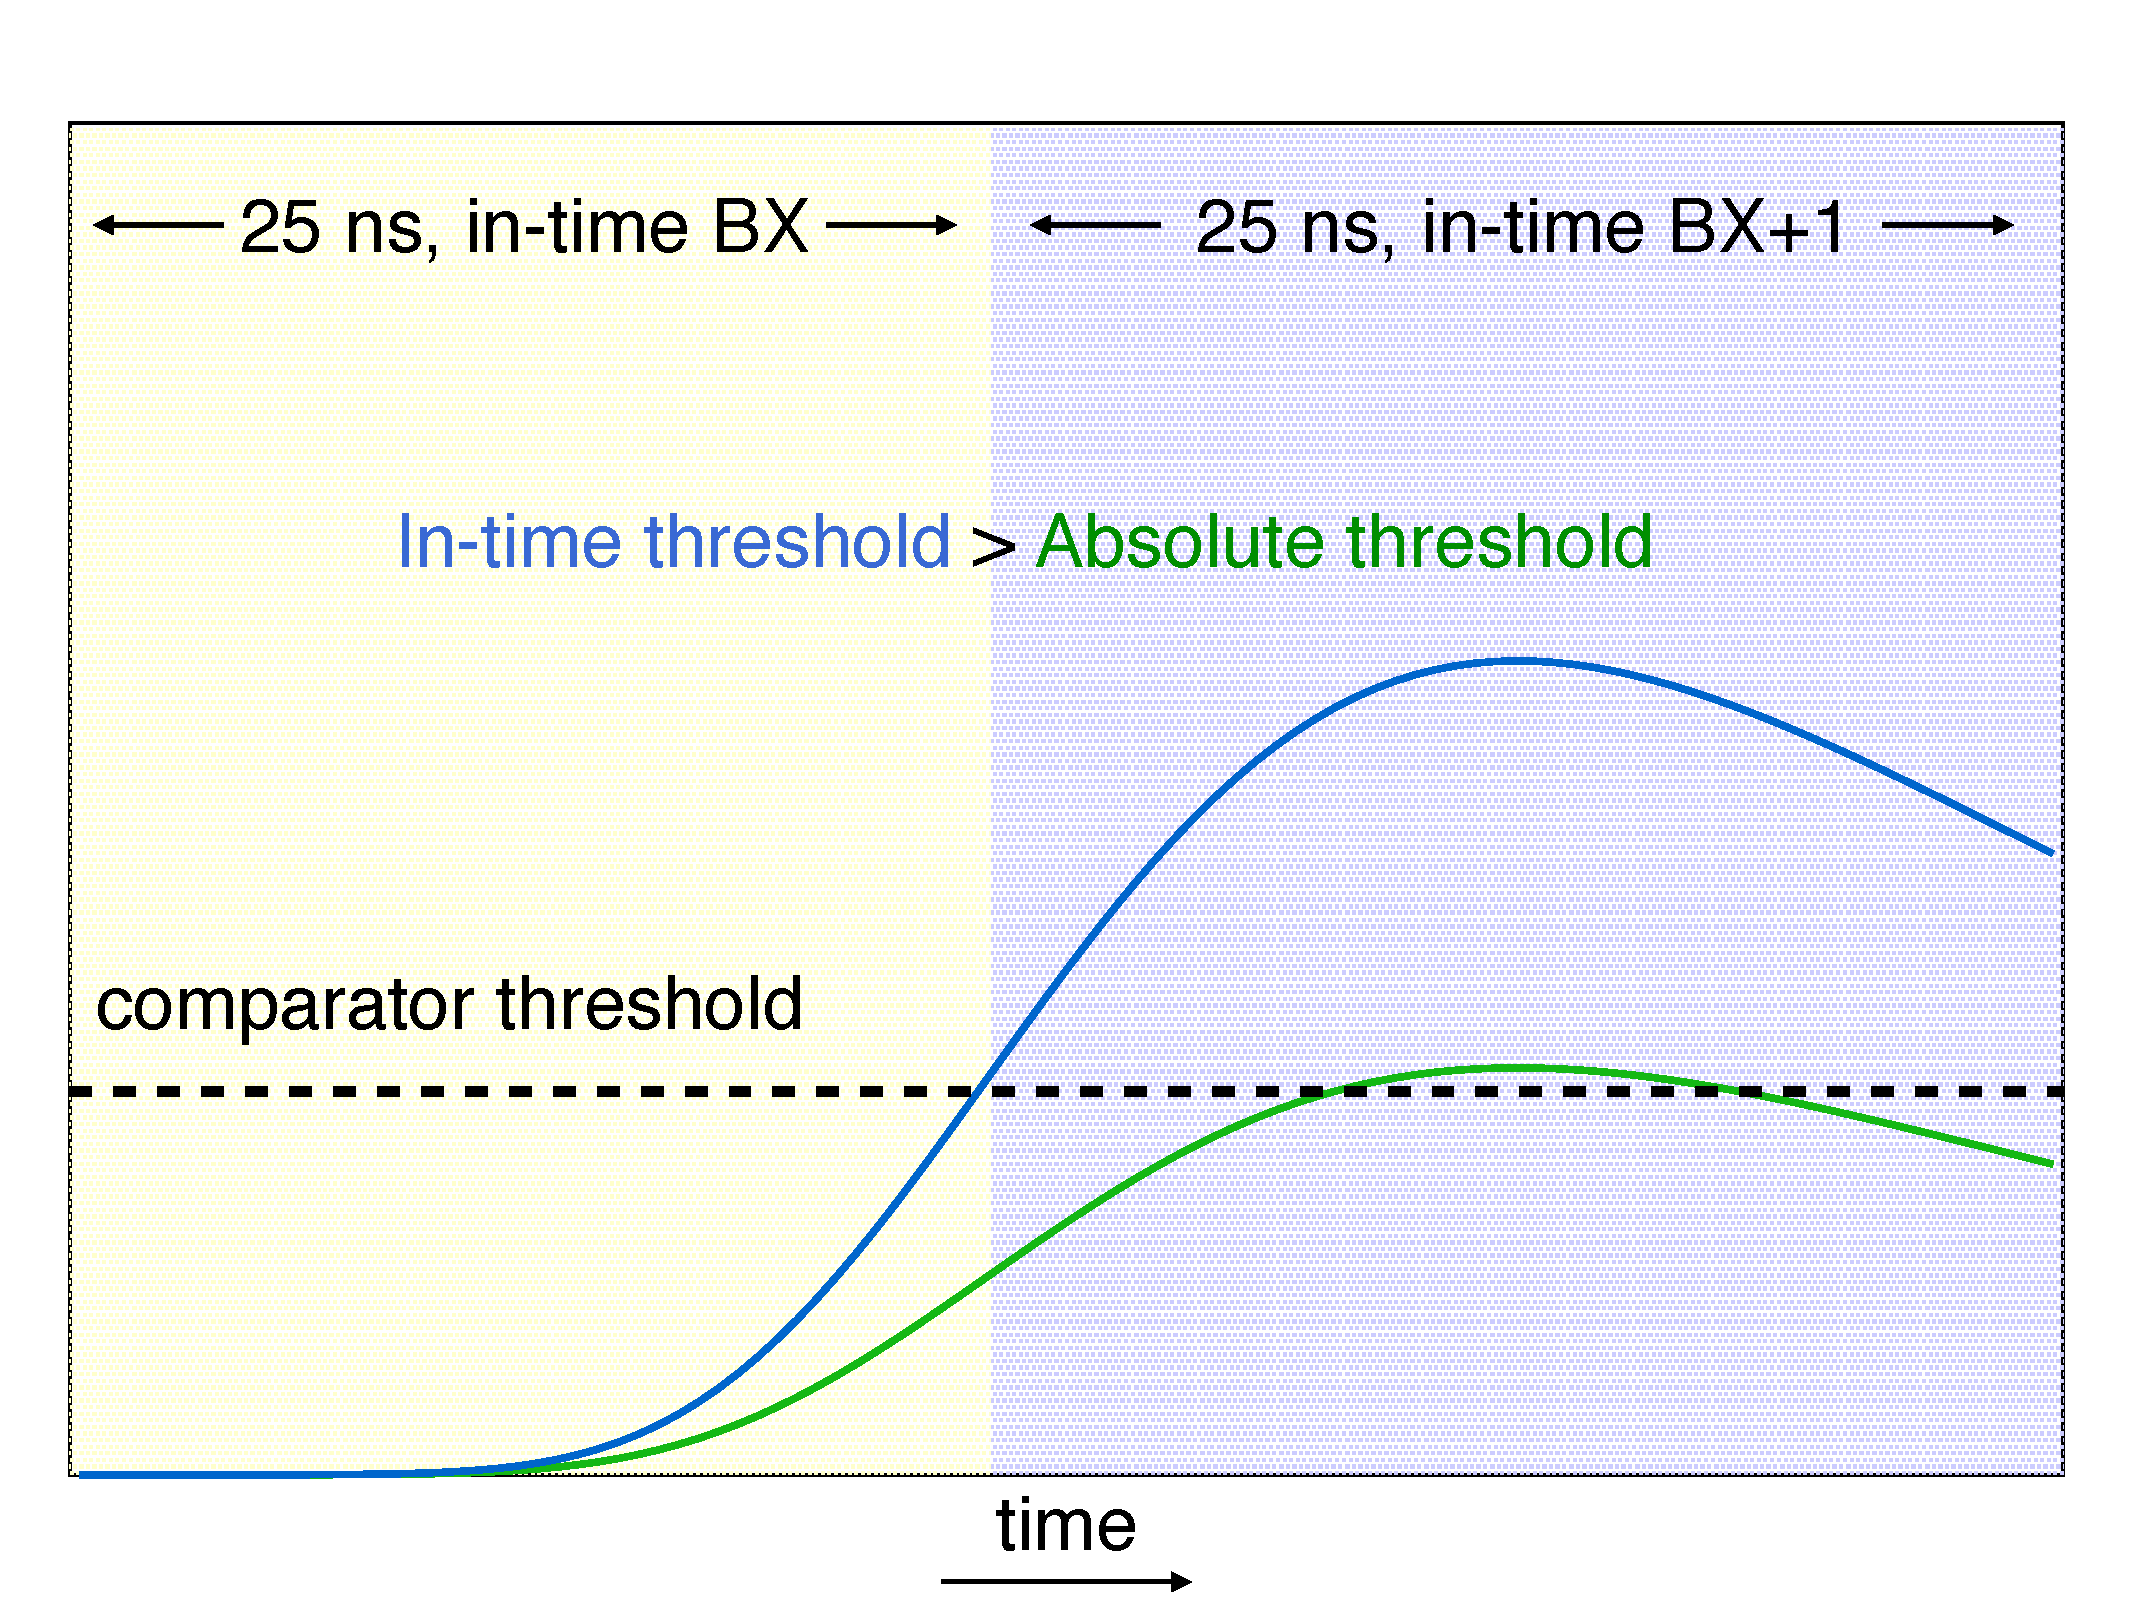
\includegraphics[width=0.45\textwidth]{\chfifteen/AbsThresold.pdf}} 
 \end{center}
 \caption{(a) Single pixel efficiency curve determined performing a scan over injected signal amplitudes (\textit{Vcal}). The curve is the result of the sum of efficiency curves for the in-time bunch crossing (BX) and the following one (BX+1). Points exceeding the 100\% efficiency are due to statistical fluctuations of the two curves in the turn-on region. The effect on the fit is negligible. (b) Diagram illustrating the difference between in-time and absolute thresholds due to the finite rise-time of the signals.}
 \label{fig:SCurve}
\end{figure}

The finite rise-time of the signal complicates the threshold measurement. 
One should distinguish the \textit{absolute threshold} defined as the comparator level above which the signal is accepted and the pixel hit is available for readout, and the \textit{in-time threshold} where the signal is fast enough to be correctly labeled by the right bunch crossing.
The difference between the two is due to \textit{time-walk} and is related to the speed of the pixel amplifier.
The absolute threshold is relevant when discussing noise and cross-talk, that is the optimum conditions under which the ROC still works. It also determines the pixel detector hit occupancy.
The in-time threshold determines the lowest amplitude signals useful for hit reconstruction and affects the position resolution.
Both thresholds can be measured using the S-curve method: for the in-time measurement the \textit{WBC} (or trigger delay) is set to the nominal value; for the absolute threshold measurement the \textit{WBC} is shifted down by one unit making the readout of the lowest amplitude (i.e. slowest) signal possible. By definition the in-time threshold is higher than the absolute. This behavior is illustrated in Fig.~\ref{fig:SCurve_b}.\\

The noise can also be measured with the S-curve method since it is proportional to the width of the region where the signal efficiency rises from 0 to 100\%.
Both noise and threshold are measured in \textit{Vcal} units, representing the parameter which determines the magnitude of the injected charge.
The calibration of the \textit{Vcal} unit itself was done during module testing using data from X-ray sources of known energies, and it varies from pixel to pixel and from ROC to ROC.
On the average, one \textit{Vcal} unit corresponds to 65.5 electrons, representing the slope of the calibration curve, whereas the average offset is -414 electrons.
However, the spreads of the two distributions are rather large, the slope parameter has an RMS of 9 and the RMS of the offset is about 570~\cite{1748-0221-4-03-P03019}.

Running this method for the whole detector is very time consuming. Instead, for each ROC the thresholds and noise are measured using only 81 pixels, which was found to be sufficient to determine the average values.
The results of the noise and threshold measurements performed in 2015 during commissioning for Run~2 will be discussed in Section~\ref{sec:commissioning}.

%%
\subsection{Optimization of the pulse height information}\label{subsec:calibPart2}
%%

\subsection*{1) Signal rise speed}

The in-time threshold depends on the amount of time-walk introduced in the amplification and shaping that occur before the signal reaches the comparator.
The speed of the pixel amplifier is controlled by \textit{Vana}, a 8-bit DAC that regulates the voltage applied to the analog part of the ROC, which can be varied in the range from 800 to 1,300\unit{mV}.
The \textit{Vana} has to be optimized such that a compromise is obtained between the desire to minimize the time-walk and the need to keep the current drawn by the analog part of the ROC, or analog current, at a reasonable level.
During module testing the optimal \textit{Vana} setting was determined for each BPix ROC by measuring directly the analog current drawn by the ROC, and then choosing the value that corresponds to 26--28\unit{mA}.
In fact, this value for the current has been found optimal to avoid exceeding the limit of the power supply.
Nevertheless, the radiation damage affects the ROC analog current and a re-calibration is necessary during operations (Fig.~\ref{fig:PixRadDamag_b}). 

\begin{figure}[!htb]
 \begin{center}
 \subfigure[]{\label{fig:VanaCalib2012_b}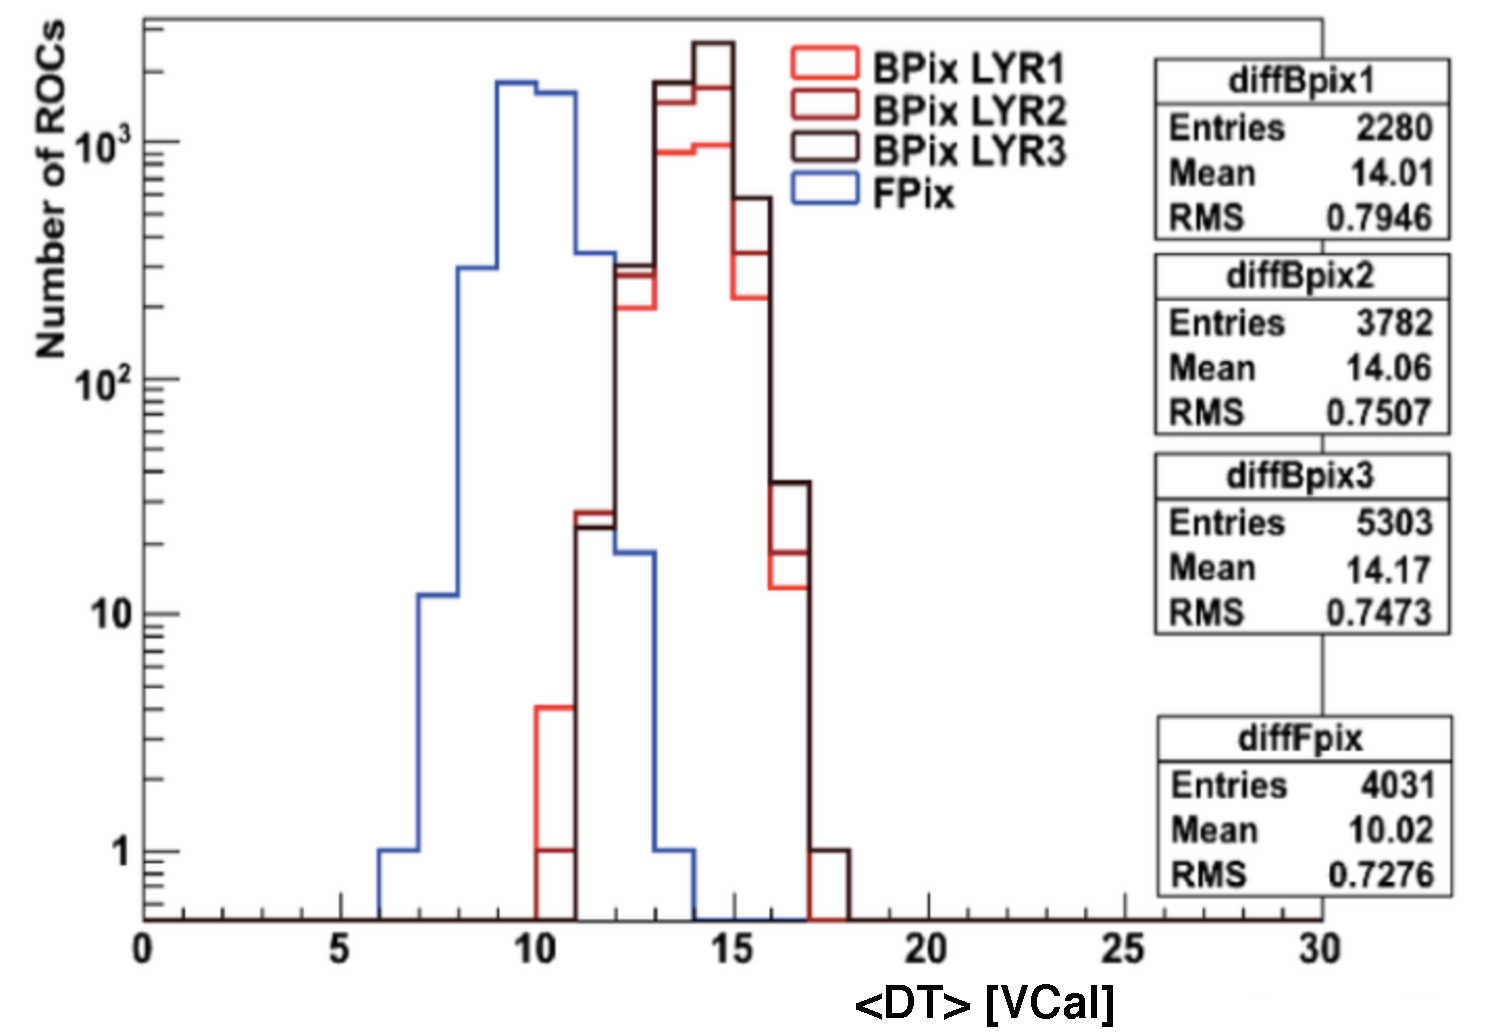
\includegraphics[width=0.45\textwidth]{\chfifteen/FinalDT2012.pdf}}
 \subfigure[]{\label{fig:VanaCalib2012_a}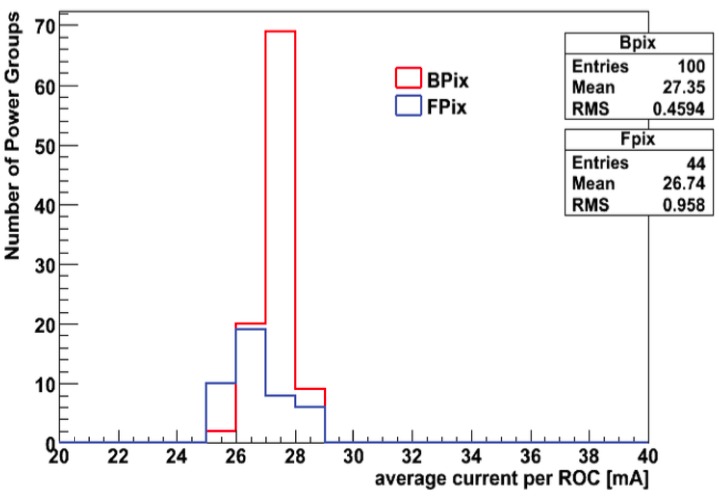
\includegraphics[width=0.45\textwidth]{\chfifteen/FinalIana2012.png}}
 \end{center}
 \caption{(a) Final distributions in DT obtained at the end of the optimization of the signal rise speed in 2012 for each barrel pixel layer and for FPix . The target DT value is chosen to reach an average analog current per ROC of 26--28\unit{mA} (b).}
 \label{fig:VanaCalib2012}
\end{figure}

Once the detector is fully assembled, it is no longer possible to access the value of the analog current for each ROC, since at this stage the only available information is the total current drawn from a single power supply, which services more than one-hundred ROCs. Thus, a procedure has been developed in the past to optimize \textit{Vana} that does not make use of this information.
The analog current can indeed be directly related to the time-walk, whose value DT can be obtained by the difference between the in-time and absolute thresholds.
The higher \textit{Vana}, the faster is the detector (smaller DT), but also the higher the current drawn by the ROC.
The target value of DT is then chosen such that the average analog current per ROC in each power group is near the optimal value of 26--28\unit{mA}.
However, the correct target for DT depends on radiation damage and temperature, so that a fixed number to target cannot be given.
Instead, one should tune the target based on the average analog current per ROC as read from the power supply.
Figure~\ref{fig:VanaCalib2012} shows the DT distributions for both BPix and FPix measured in 2012, as well as the corresponding average analog current per ROC.
For BPix, a target DT value of 14 \textit{Vcal} was found to be sufficient to reach the optimal current.

In order to optimize the DT, the calibration is implemented as an iterative procedure, which makes use of the in-time and absolute threshold measurements given by the S-curve method.
It has been found from calibrations performed during Run~1 that the relation $\Delta(\mathrm{DT}) = \mathrm{DT} - \mathrm{DT}_{target} \simeq \Delta{Vana}$ holds~\cite{Gaz:2013pja}.
Using this relation, the new \textit{Vana} settings are computed for each iteration and then downloaded to the ROCs for the next iteration. In each iteration, the absolute threshold and charge injection timing has to be re-calibrated (step 5 in Section~\ref{subsec:calibPart1}) because of their dependence on \textit{Vana}. 
Figure~\ref{fig:VanaCalib} illustrates the evolution of the \textit{Vana} settings with the iterations showing how these converge to the value corresponding to the target DT.

\begin{figure}[!htb]
\begin{center}
 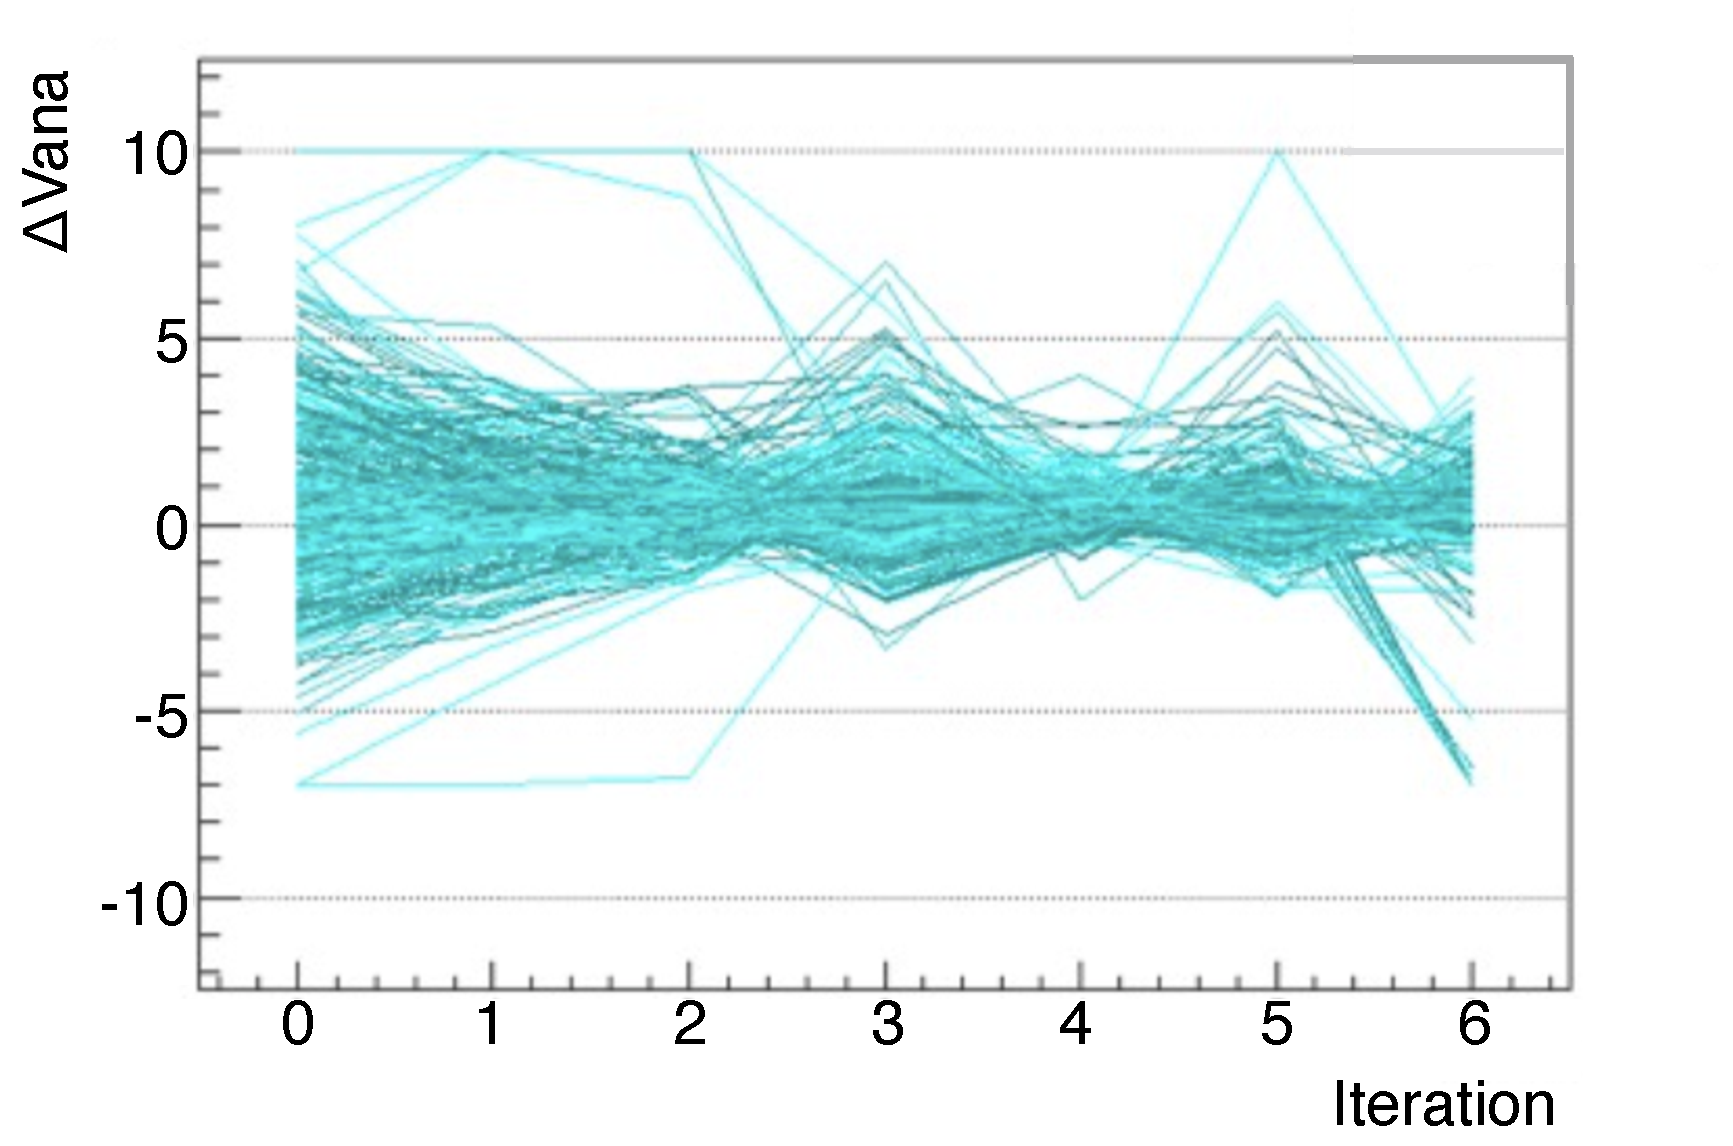
\includegraphics[width=0.6\textwidth]{\chfifteen/VanaCalibration-3.pdf}
 \end{center}
 \caption{Example of optimization of the signal rise speed obtained from tests conducted in the clean room during LS1. The evolution of the \textit{Vana} settings for some ROCs with the iterations is shown and illustrates how these converge to the values corresponding to the target DT. }
 \label{fig:VanaCalib}
\end{figure}

\subsection*{2) Threshold minimization}

This step is meant to set the threshold of each ROC at the lowest practical value, so that the threshold is low enough to detect low amplitude signals and ensure high hit resolution,
but above the noise level.
The procedure for minimizing the threshold starts setting a large value of the comparator threshold (for instance 50 \textit{Vcal}) in each ROC such that it is above the level of noise.
The threshold is then lowered by 2 units and a pixel alive test or S-curve is run to check wether a ROC is failing because the threshold is too low and noise occurs.
The procedure is iterated until all ROCs reach the minimum achievable value. For each iteration the charge injection timing has to be re-optimized as well.
Several scripts have been implemented during LS1 to automatize this time consuming procedure. An example of the results from tests conducted in the clean room during LS1 is shown in Fig.~\ref{fig:ThrCalibLS1}.
The final threshold and noise distributions for the whole detector obtained with this method before the start of data-taking in 2015 are discussed in Section~\ref{sec:commissioning}.

\begin{figure}[!htb]
\begin{center}
 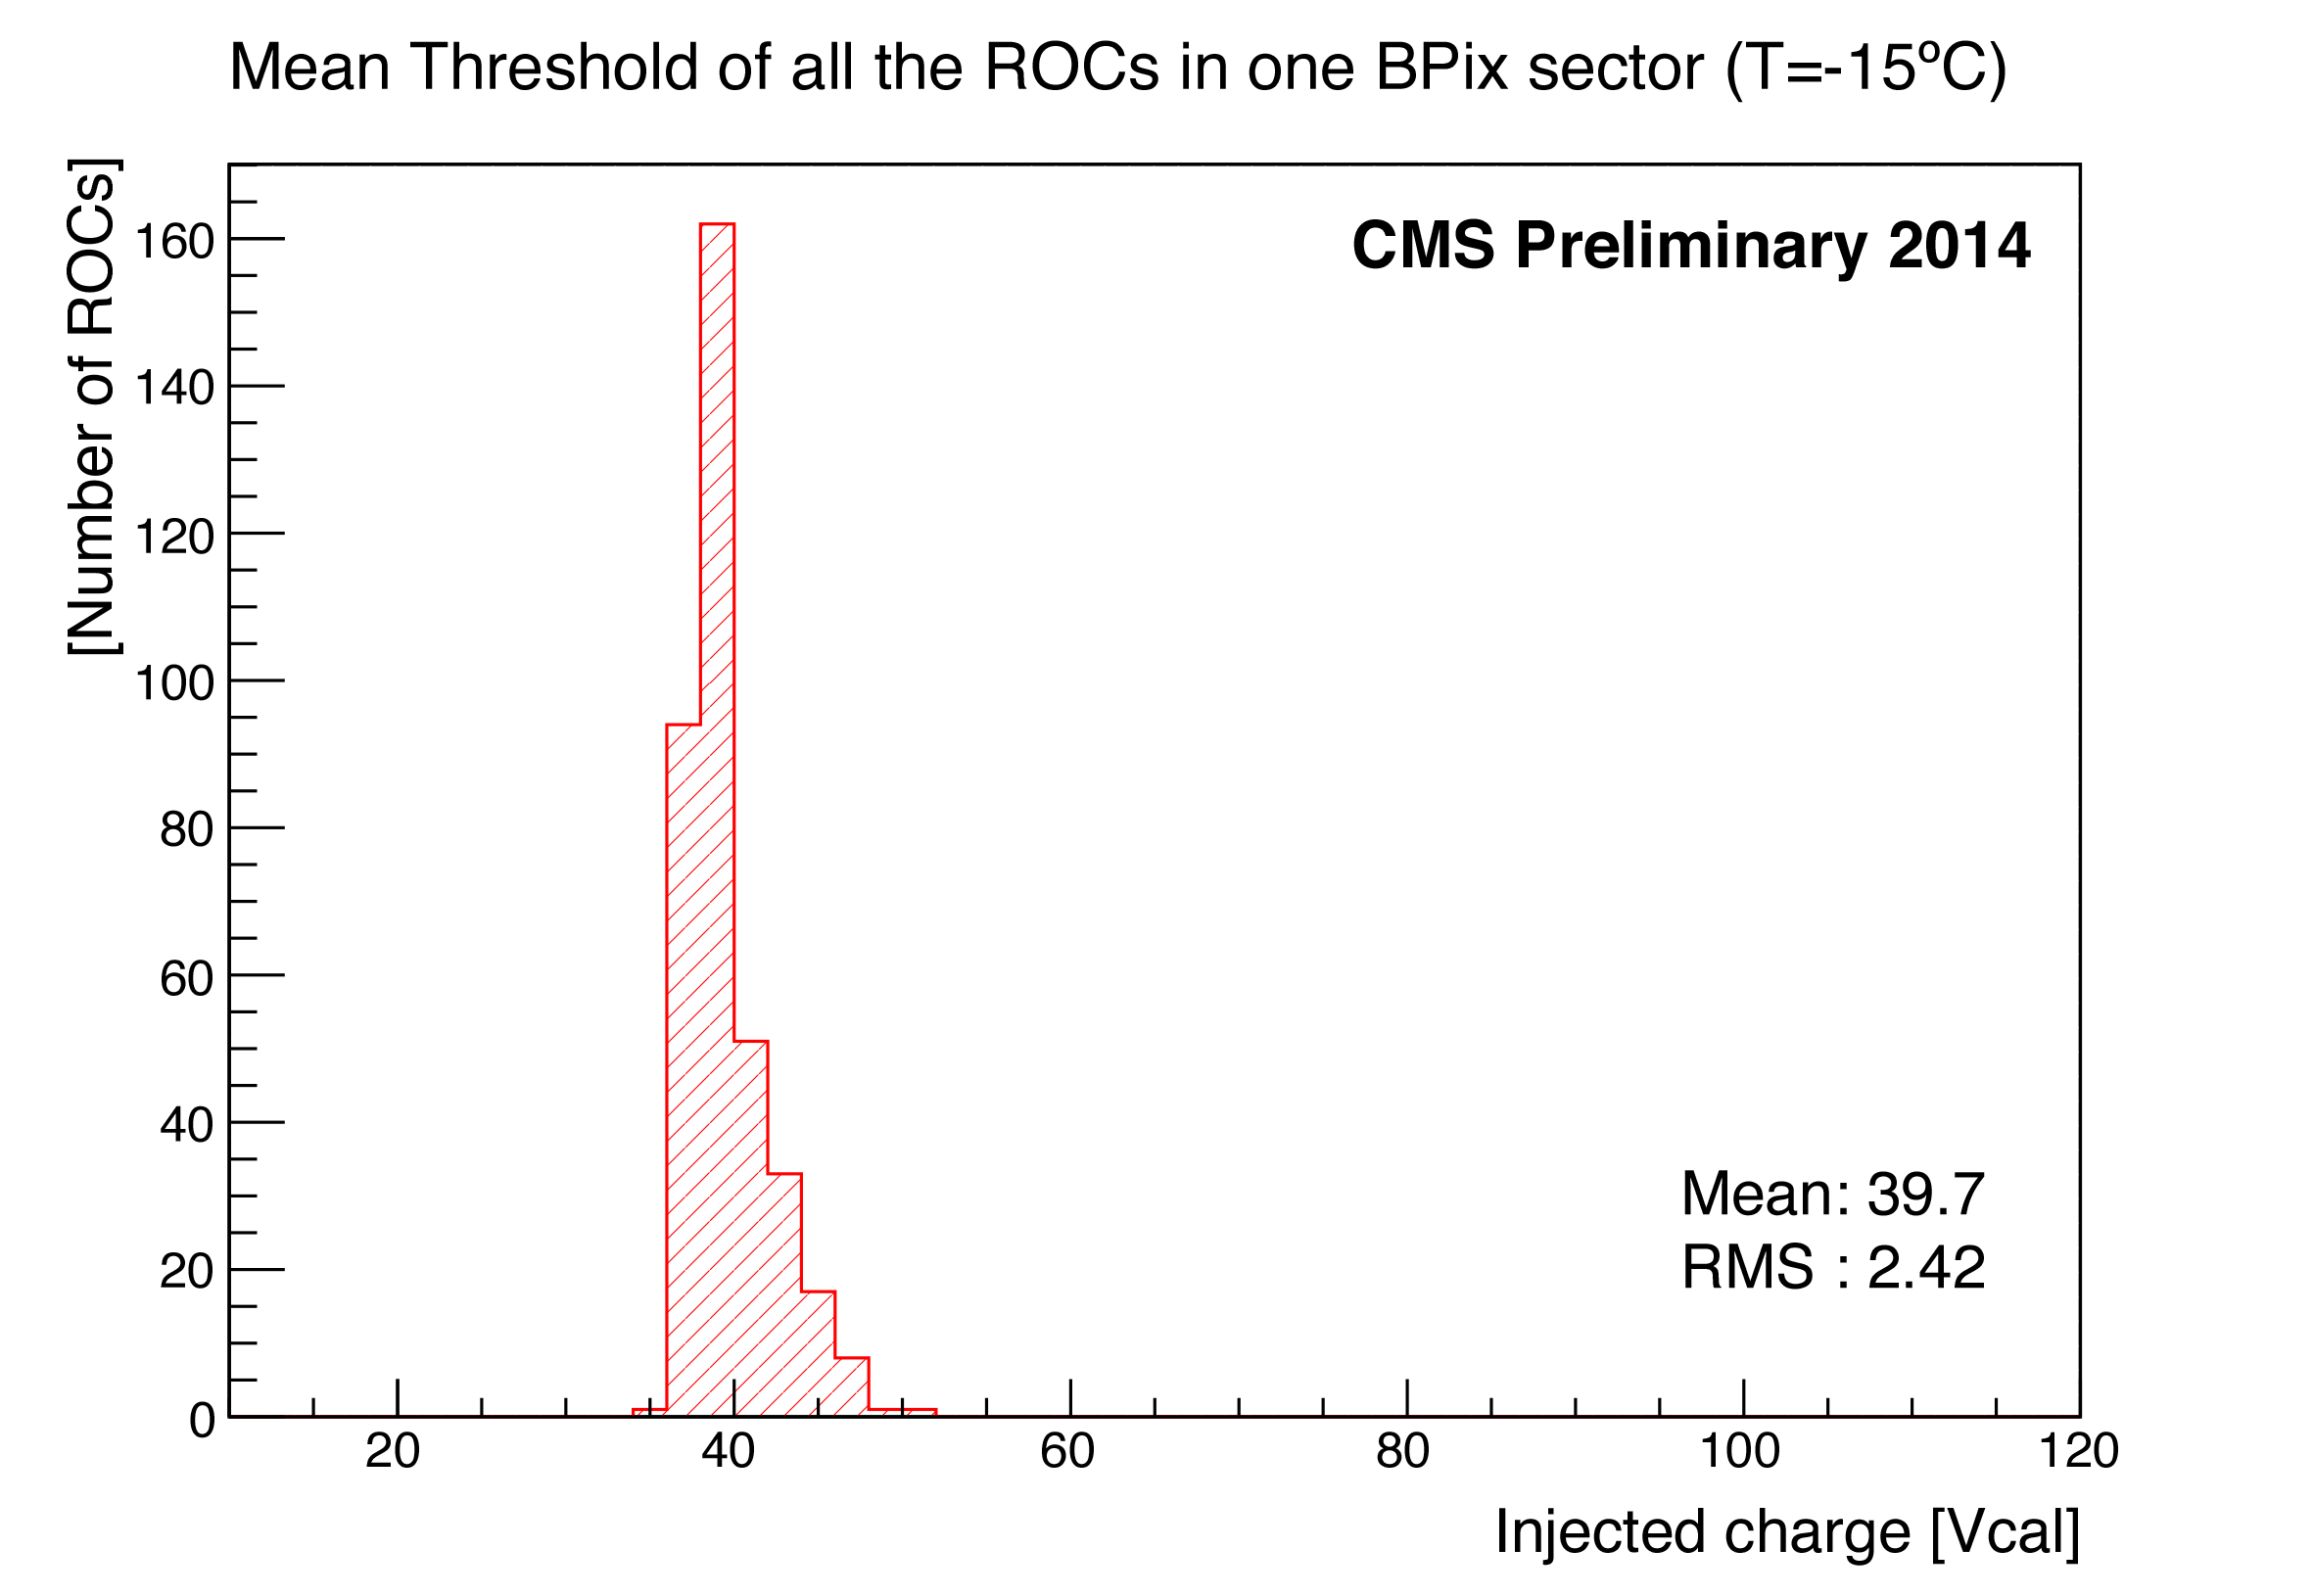
\includegraphics[width=0.45\textwidth]{\chfifteen/MeanThresholdLS1.png}
 \end{center}
 \caption{Distribution of the minimized thresholds for all the ROCs in one BPix sector. The measurement was performed at -15\unit{$^\circ$C} coolant temperature in the clean room during LS1.}
 \label{fig:ThrCalibLS1}
\end{figure}

\subsection*{3) Analog signal response calibration}

The final part of the calibration procedure is aimed at maximizing the range and linearity of the detector.
In fact, the hit position is interpolated from the charge information of all pixels in a cluster. For a precise position resolution it is therefore crucial to know for each pixel the exact response curve (or pixel gain) that converts the analog pulse height (in ADC counts) into the corresponding charge.
%Furthermore, a linear response is preferable in order to simplify its modeling and hence, reduce uncertainties in the position resolution.
The response curve is measured by injecting signals with increasing amplitudes to each pixel and measuring the analog pulse height.
Before this calibration, the linearity of the response curve is optimized by adjusting few DAC registers in the ROC.
The linearity is required for two reasons. On one hand the non-linear behavior in the low range does not allow to reconstruct the charge of the signal, on the other hand fewer parameters have to be stored in the data base.
The \textit{VhldDel} register controls the delay that is applied to each pulse before its height is sampled and stored in the sample and hold capacitance until the readout mechanism is started from the periphery.
The supply voltage of the sample and hold circuit is regulated by the \textit{Vsf} register.

Figure~\ref{fig:VhldDel} shows the pulse height as a function of \textit{VhldDel} settings at low, medium, and high values of \textit{Vsf}, for a fixed injected signal amplitude.
A good \textit{Vsf} value is one for which this curve rises and then falls so that the pulse heights at the two endpoints (lowest and highest \textit{VhldDel}) are equal.
The figure also includes a plot of these endpoints as a function of \textit{Vsf}; the rightmost intersection point is the \textit{Vsf} value chosen. Low values of \textit{Vsf}, below $\sim 90$ are discarded because they are found to be not optimal for a correct readout. After choosing the \textit{Vsf} value, \textit{VhldDel} is set to the value that maximizes the pulse height.
%When charge is injected with Vcal = 250 on the low scale, these Vsf and VHldDel settings are found to give good linearity in pulse height vs. injected charge, while not drawing too much power.

\begin{figure}[!htb]
\begin{center}
 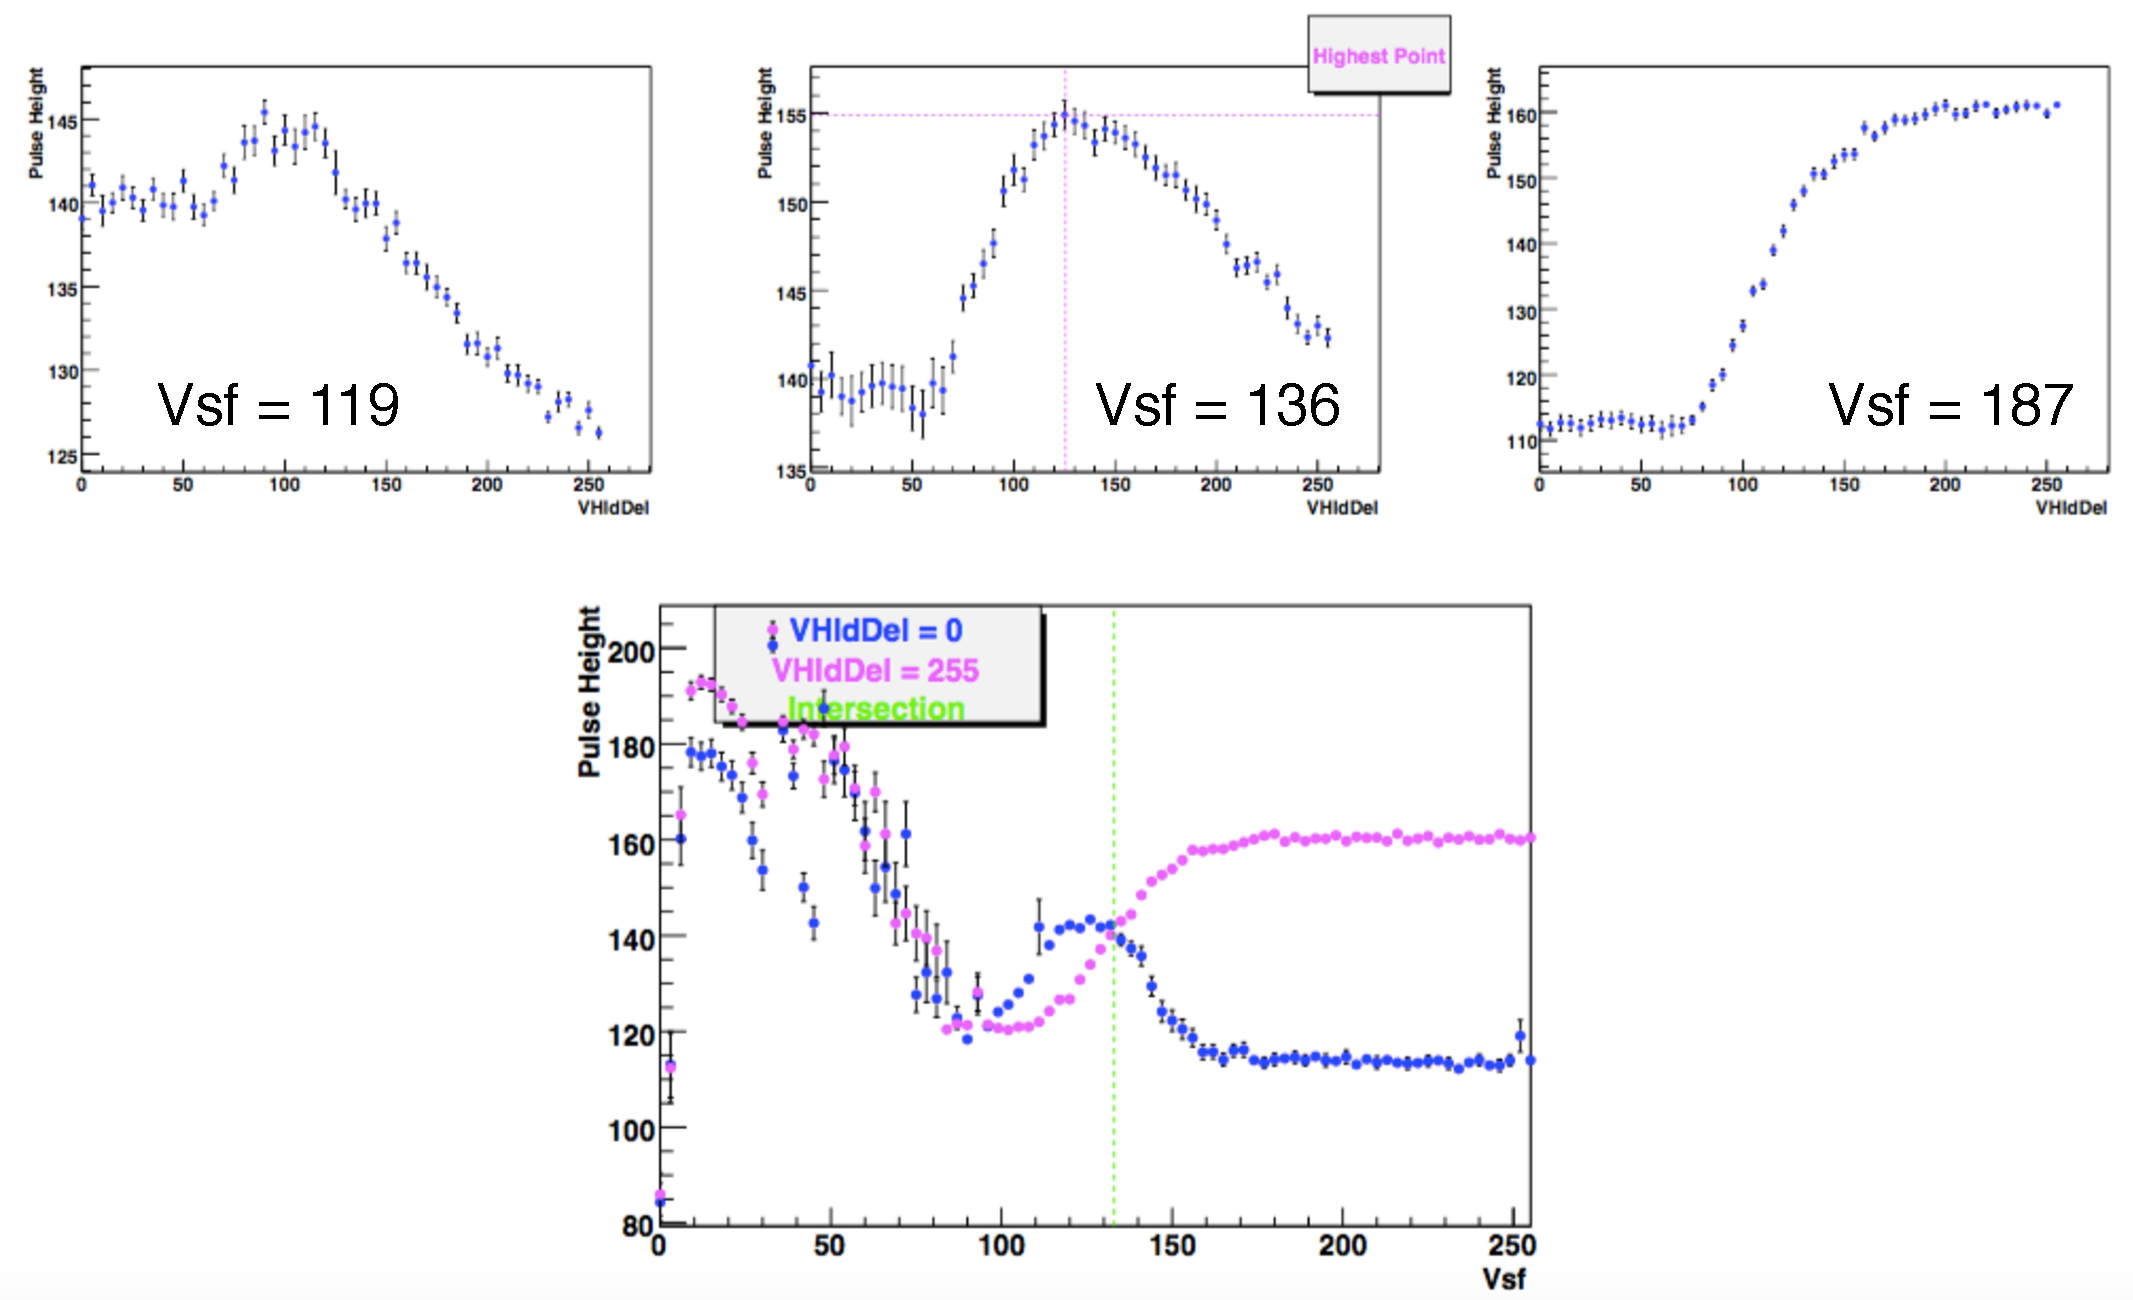
\includegraphics[width=\textwidth]{\chfifteen/VsfVHldDel.pdf}
 \end{center}
 \caption{Top row: pulse height as a function of \textit{VhldDel} for low, medium, and high values of \textit{Vsf}. As \textit{Vsf} increases, the right endpoint shifts to the right.
 The best \textit{Vsf} value is the one for which the pulse heights measured at the extremes of the \textit{VhldDel} range are equal.
 Bottom plot: pulse height at the extremes, as a function of \textit{Vsf}. Low values of \textit{Vsf} are discarded because not optimal.}
 \label{fig:VhldDel}
\end{figure}

Several ROC DAC settings also affect the scaling of the pulse height signal that is sent out to the FED. The difference in recorded pulse height between a small and large amount of collected charge should be preferably large.
However, the pulse height signal should not go too low to be confused with the UB level, nor too high to exceed the FED's dynamic range.
Hence, a calibration is run to optimize these settings as well.

After these fine adjustments, the measurement of the response curve for each pixel is performed. For each pixel about 30 charge values are injected. 
During the scan, the acquired data is stored in binary files and is later analyzed offline. All pixels have to be calibrated, therefore, the procedure is time consuming and takes about 8 hours for the whole detector.
An example of such measurement for one pixel is shown in Fig.~\ref{fig:GainCalib}. For comparison, an example exhibiting a non-linear behavior for a non optimal \textit{Vsf} setting is also shown.
The saturation in the high range is less important since it occurs for charges of more than 30-40 ke.

\begin{figure}[!htb]
 \begin{center}
 \subfigure[]{\label{fig:GainCalib_a}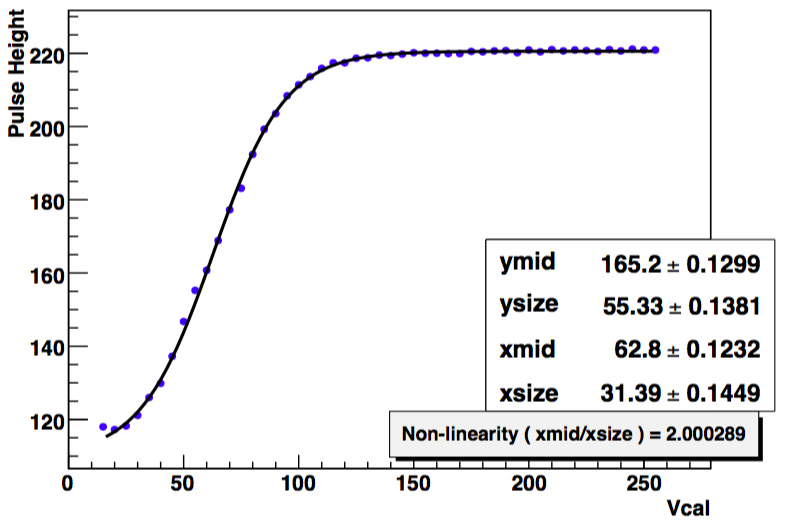
\includegraphics[width=0.45\textwidth]{\chfifteen/GainCalibNonLin.png}}
 \subfigure[]{\label{fig:GainCalib_b}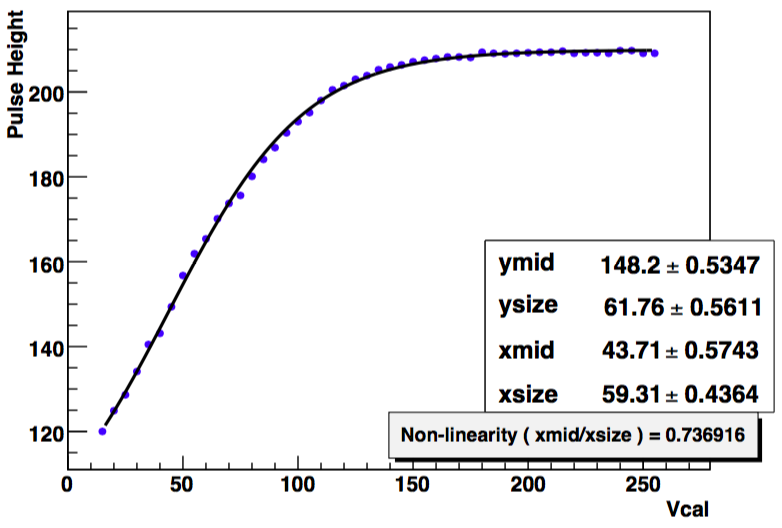
\includegraphics[width=0.45\textwidth]{\chfifteen/GainCalibLin.png}}
 \end{center}
 \caption{Examples of pixel response curve (gain calibration) representing the scan of the pulse height as a function of \textit{Vcal}. The scan on the left presents poor linearity as performed for a not optimal value of \textit{Vsf}.}
 \label{fig:GainCalib}
\end{figure}

The pixel response curves are parametrized with the following function:

\begin{equation}
PH = f(Vcal) = y_{mid} + y_{size} \cdot \mathrm{tanh}\left( \frac{Vcal - x_{mid}}{x_{size}} \right),
\end{equation}

where $PH$ is the recorded pulse height,
($x_{mid}$, $y_{mid}$) is the point at the center of the quasi-linear rise region of the hyperbolic tangent,
$x_{size}$ and $y_{size}$ are the horizontal and vertical scales of the quasi-linear region, respectively.
If $x_{mid}/x_{size} \approx 1$, the response curve is linear in the whole region of interest.
Thus, the linear region below the saturation is
parametrized by only the slope (gain) and offset (pedestal) of a linear fit.
%The curve is approximately linear below saturation at about 45,000 electrons and can be parametrized by the slope (gain) and offset (pedestal) of a linear fit.
These parameters are then used in the data reconstruction. 
The results of the gain calibration performed for the whole detector before the start of data-taking in 2015 are discussed in Section~\ref{sec:commissioning}.

%%%%%%%%%%%
\section{Re-commissioning for LHC Run 2}\label{sec:commissioning}
%%%%%%%%%%%

The barrel pixel detector was installed back into CMS on 8th December 2014.
The operations, described in Section~\ref{sec:BPixInst}, were coordinated by the PSI and UZH teams (Fig.~\ref{fig:BPixInst}), and were completed in only 5 days.
After that, the FPix detector was also installed following a similar check out procedure as for BPix so that most work was already completed before Christmas.
The full pixel detector was re-commissioned in January 2015 within about a fortnight using the procedure described in the previous section.
Section~\ref{sec:FinalBPixCalib} presents the results of the detector calibrations performed for the whole detector at low temperature after the installation.
Finally, in Section~\ref{sec:BPixPerf2015}, the detector performance at the beginning of the LHC Run~2 are discussed.

\begin{figure}[!htb]
 \begin{center}
 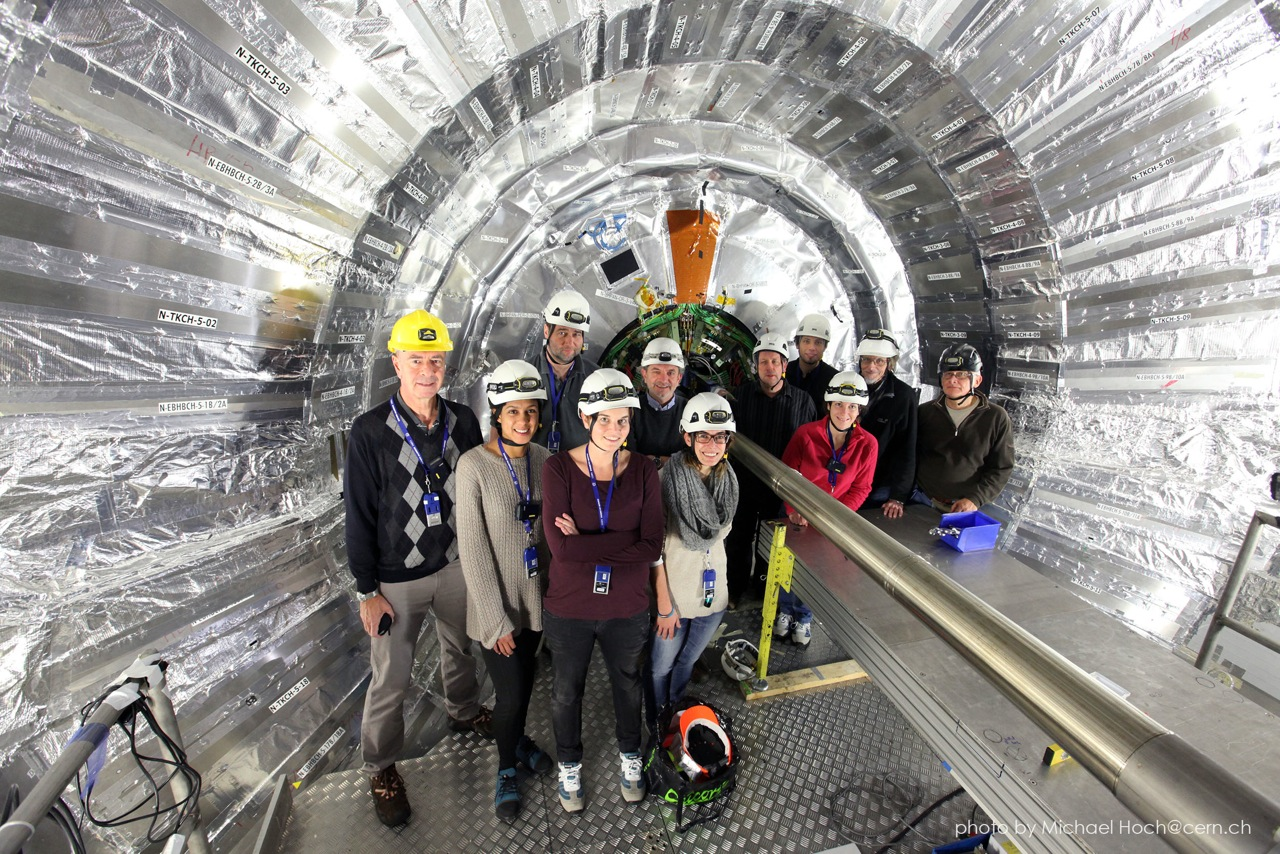
\includegraphics[width=0.8\textwidth]{\chfifteen/aIMG_6479ts.jpeg}
 \end{center}
 \caption{Pictures taken on the CMS underground platform after the re-installation of the barrel pixel detector in December 2014. The operations were coordinated by the PSI and UZH teams.}
 \label{fig:BPixInst}
\end{figure}

\subsection{Installation into CMS}\label{sec:BPixInst}

The barrel pixel detector re-installation into CMS took place only three months later than originally planned due to the incident mentioned in the previous section. 
Particular care was given to the centering of the detector with respect to the new beam pipe, required for the upgraded pixel detector planned for Spring 2017 (Chapter~\ref{ch:Phase1Intro}),
since before it had been slightly shifted irradiating one side stronger than the other.
Figure~\ref{fig:BPixInst2} shows pictures taken on the CMS underground platform illustrating the operations conducted in the first two days.
The first day, each half of the detector was moved inside a transport box from the clean room and lowered down to the cavern through the main shaft.
A system with rails on top and bottom inside CMS had been designed to insert the pixel detector and the supply tubes along the beam pipe.
%This is visible in the picture in the middle of the bottom row in Fig.~\ref{fig:BPixInst2}.
The transport box with the detector was lifted to the insertion table and the rail system inside the box was joint with the rail system inside CMS using temporary extension rails.
In this way, the detector could slide out of the transport box into its final position.
The following day, all cooling loops, power cables and fibers were connected, and first attempts to power the detector and to test a sector were made.
A picture of the detector in the final position with all power and control cables and optical fibers connected is shown in Fig.~\ref{fig:BPixInst3}.
%The detector was then checked out over the course of the next three days at room temperature of about 16\unit{$^\circ$C}.
%The FPix detector was installed on 13th December 2014 following a similar check-out procedure as for BPix so that most work was already completed before Christmas.
%The third and outermost FPix disk that had so far been empty was equipped with a pilot system for the upgrade of the pixel detector 
%The tracker bulkheads were closed on 29th January to end LS1.
%Basic calibrations for BPix check out after installation
%delay25 chip calibration to adjust the parameters for module programming
%quickly check out the status of the optical readout system looking at the FED baseline
%AOH bias and gain, TBM and ROC UB calibrations for adjusting
%Address level calibration

\begin{figure}[!htb]
 \begin{center}
 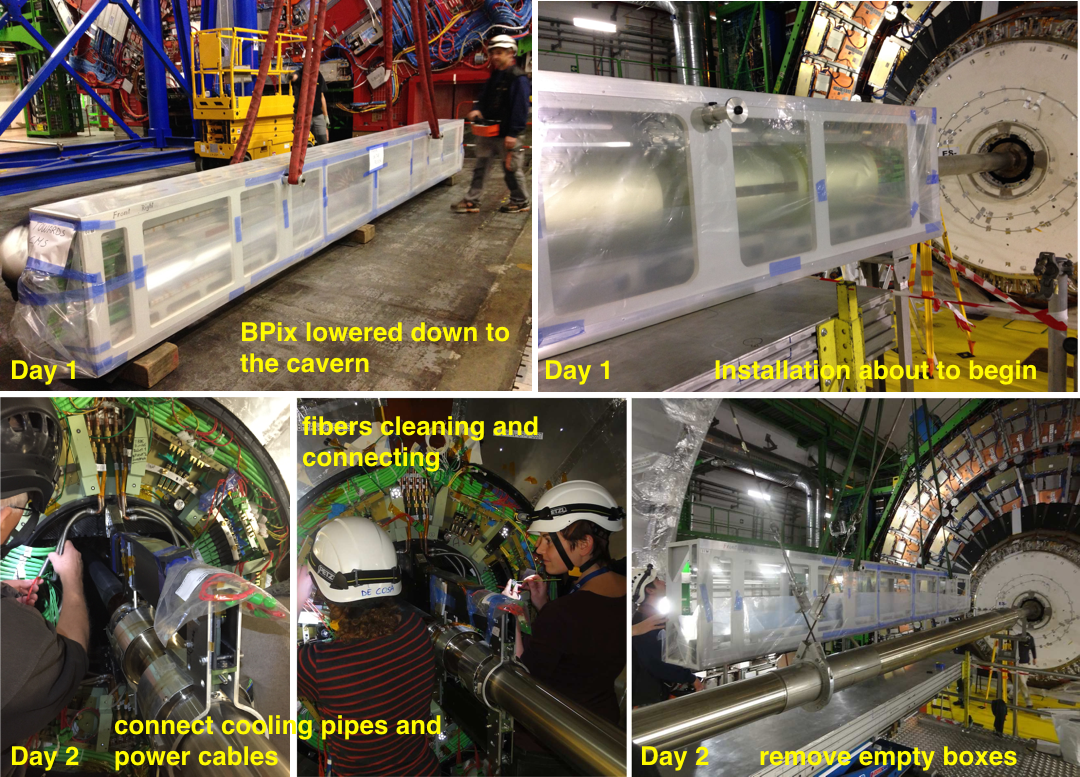
\includegraphics[width=0.8\textwidth]{\chfifteen/BPixInstallation2015.png}
 \end{center}
 \caption{Pictures illustrating the steps of the BPix re-installation in December 2014. The operation has been completed in 2 days.}
 \label{fig:BPixInst2}
\end{figure}

\begin{figure}[!htb]
 \begin{center}
 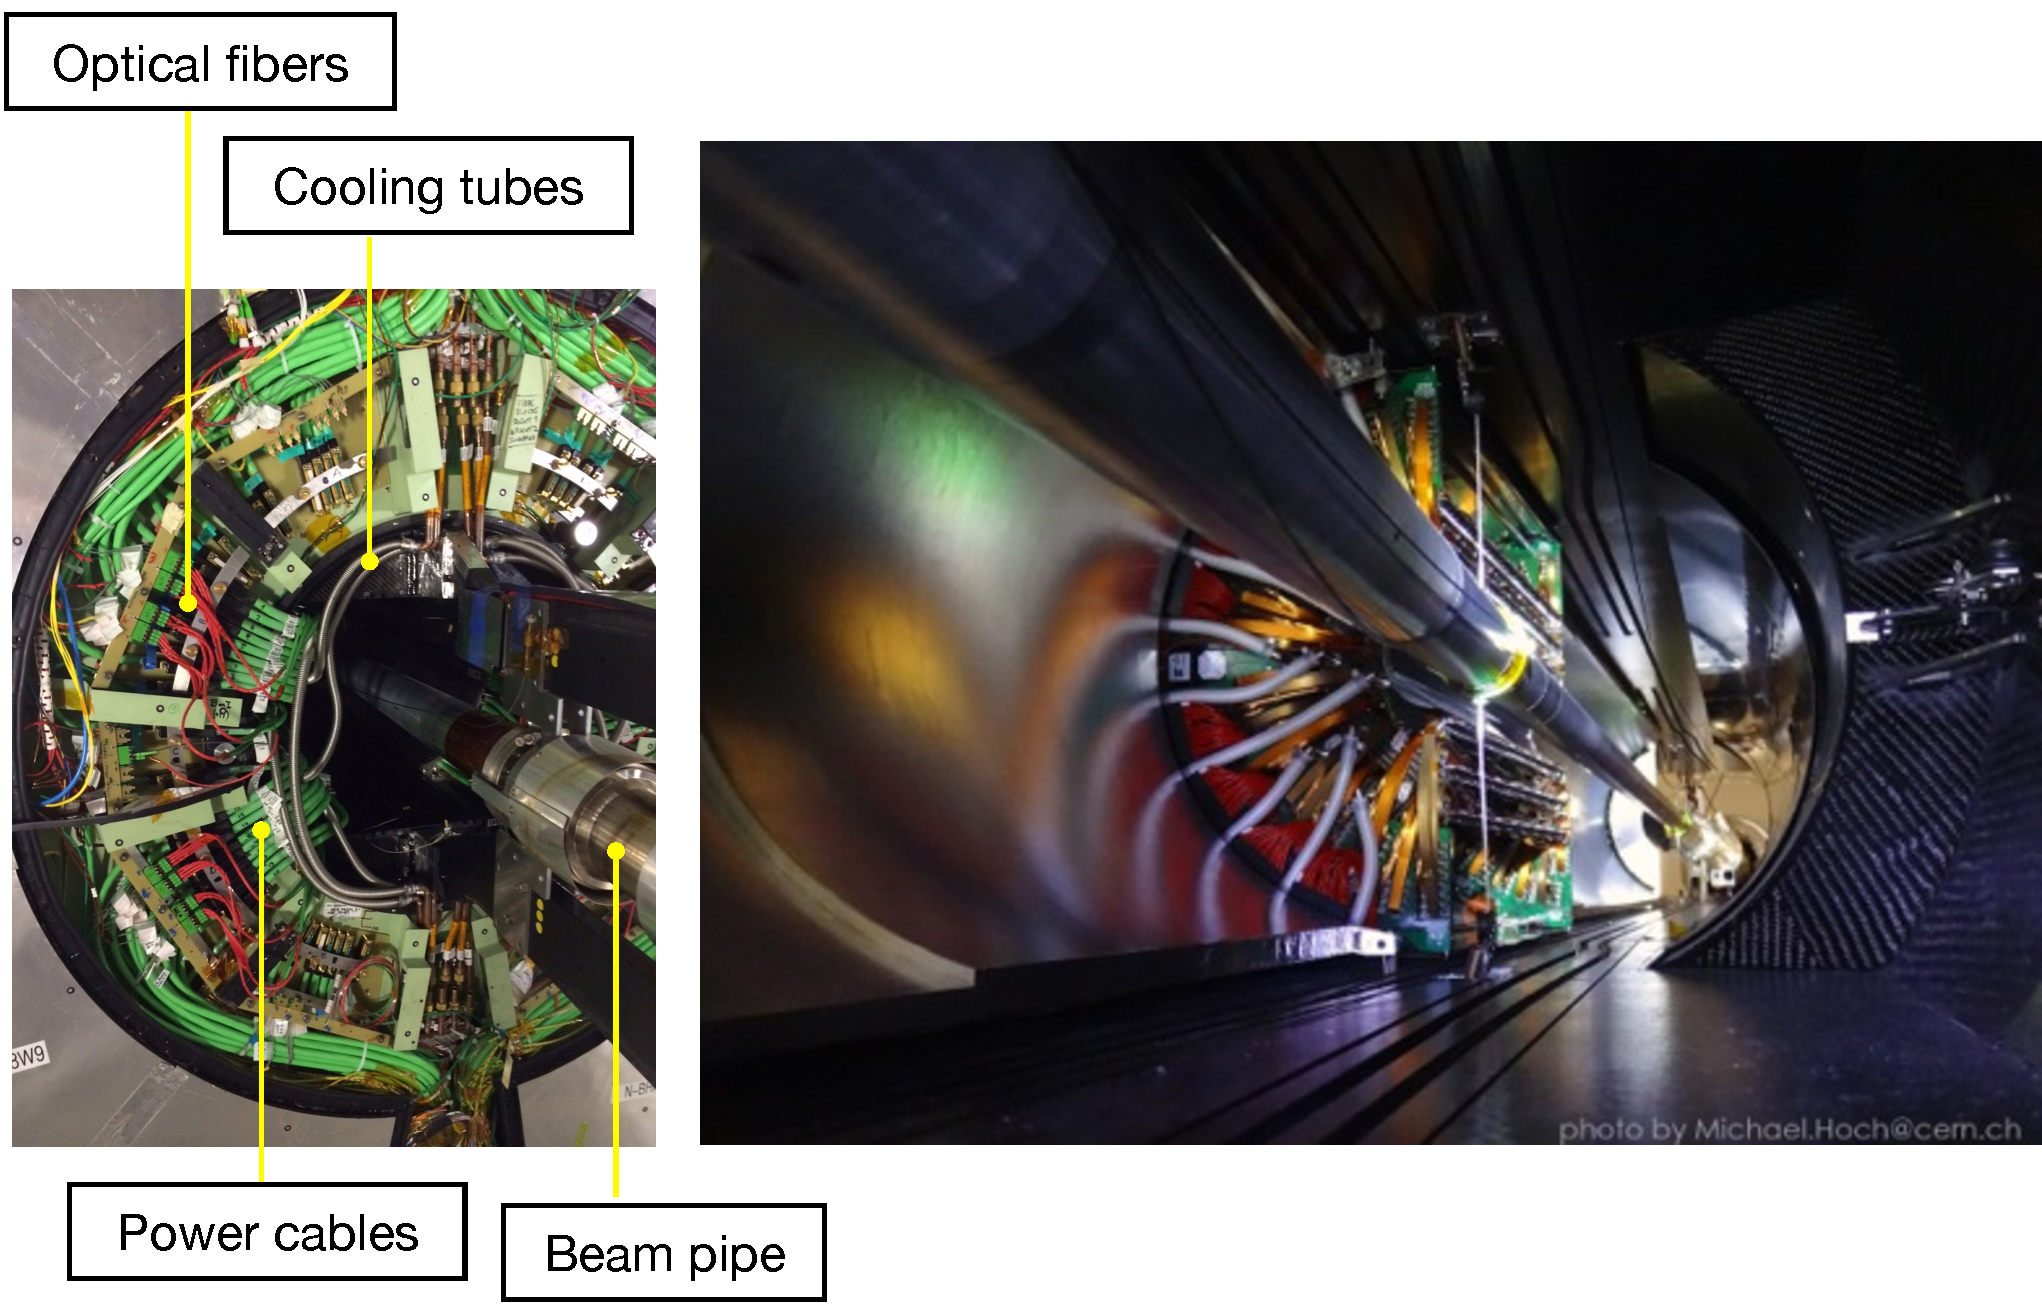
\includegraphics[width=0.8\textwidth]{\chfifteen/BPixInstallation2015-2.pdf}
 \end{center}
 \caption{View of half of the barrel pixel detector in its final position inside CMS. The central beam pipe and the detector end-flanges with cooling lines and power and signal cables can be seen.}
 \label{fig:BPixInst3}
\end{figure}

%\begin{wrapfigure}{R}{0.4\textwidth}
 %\centering
 %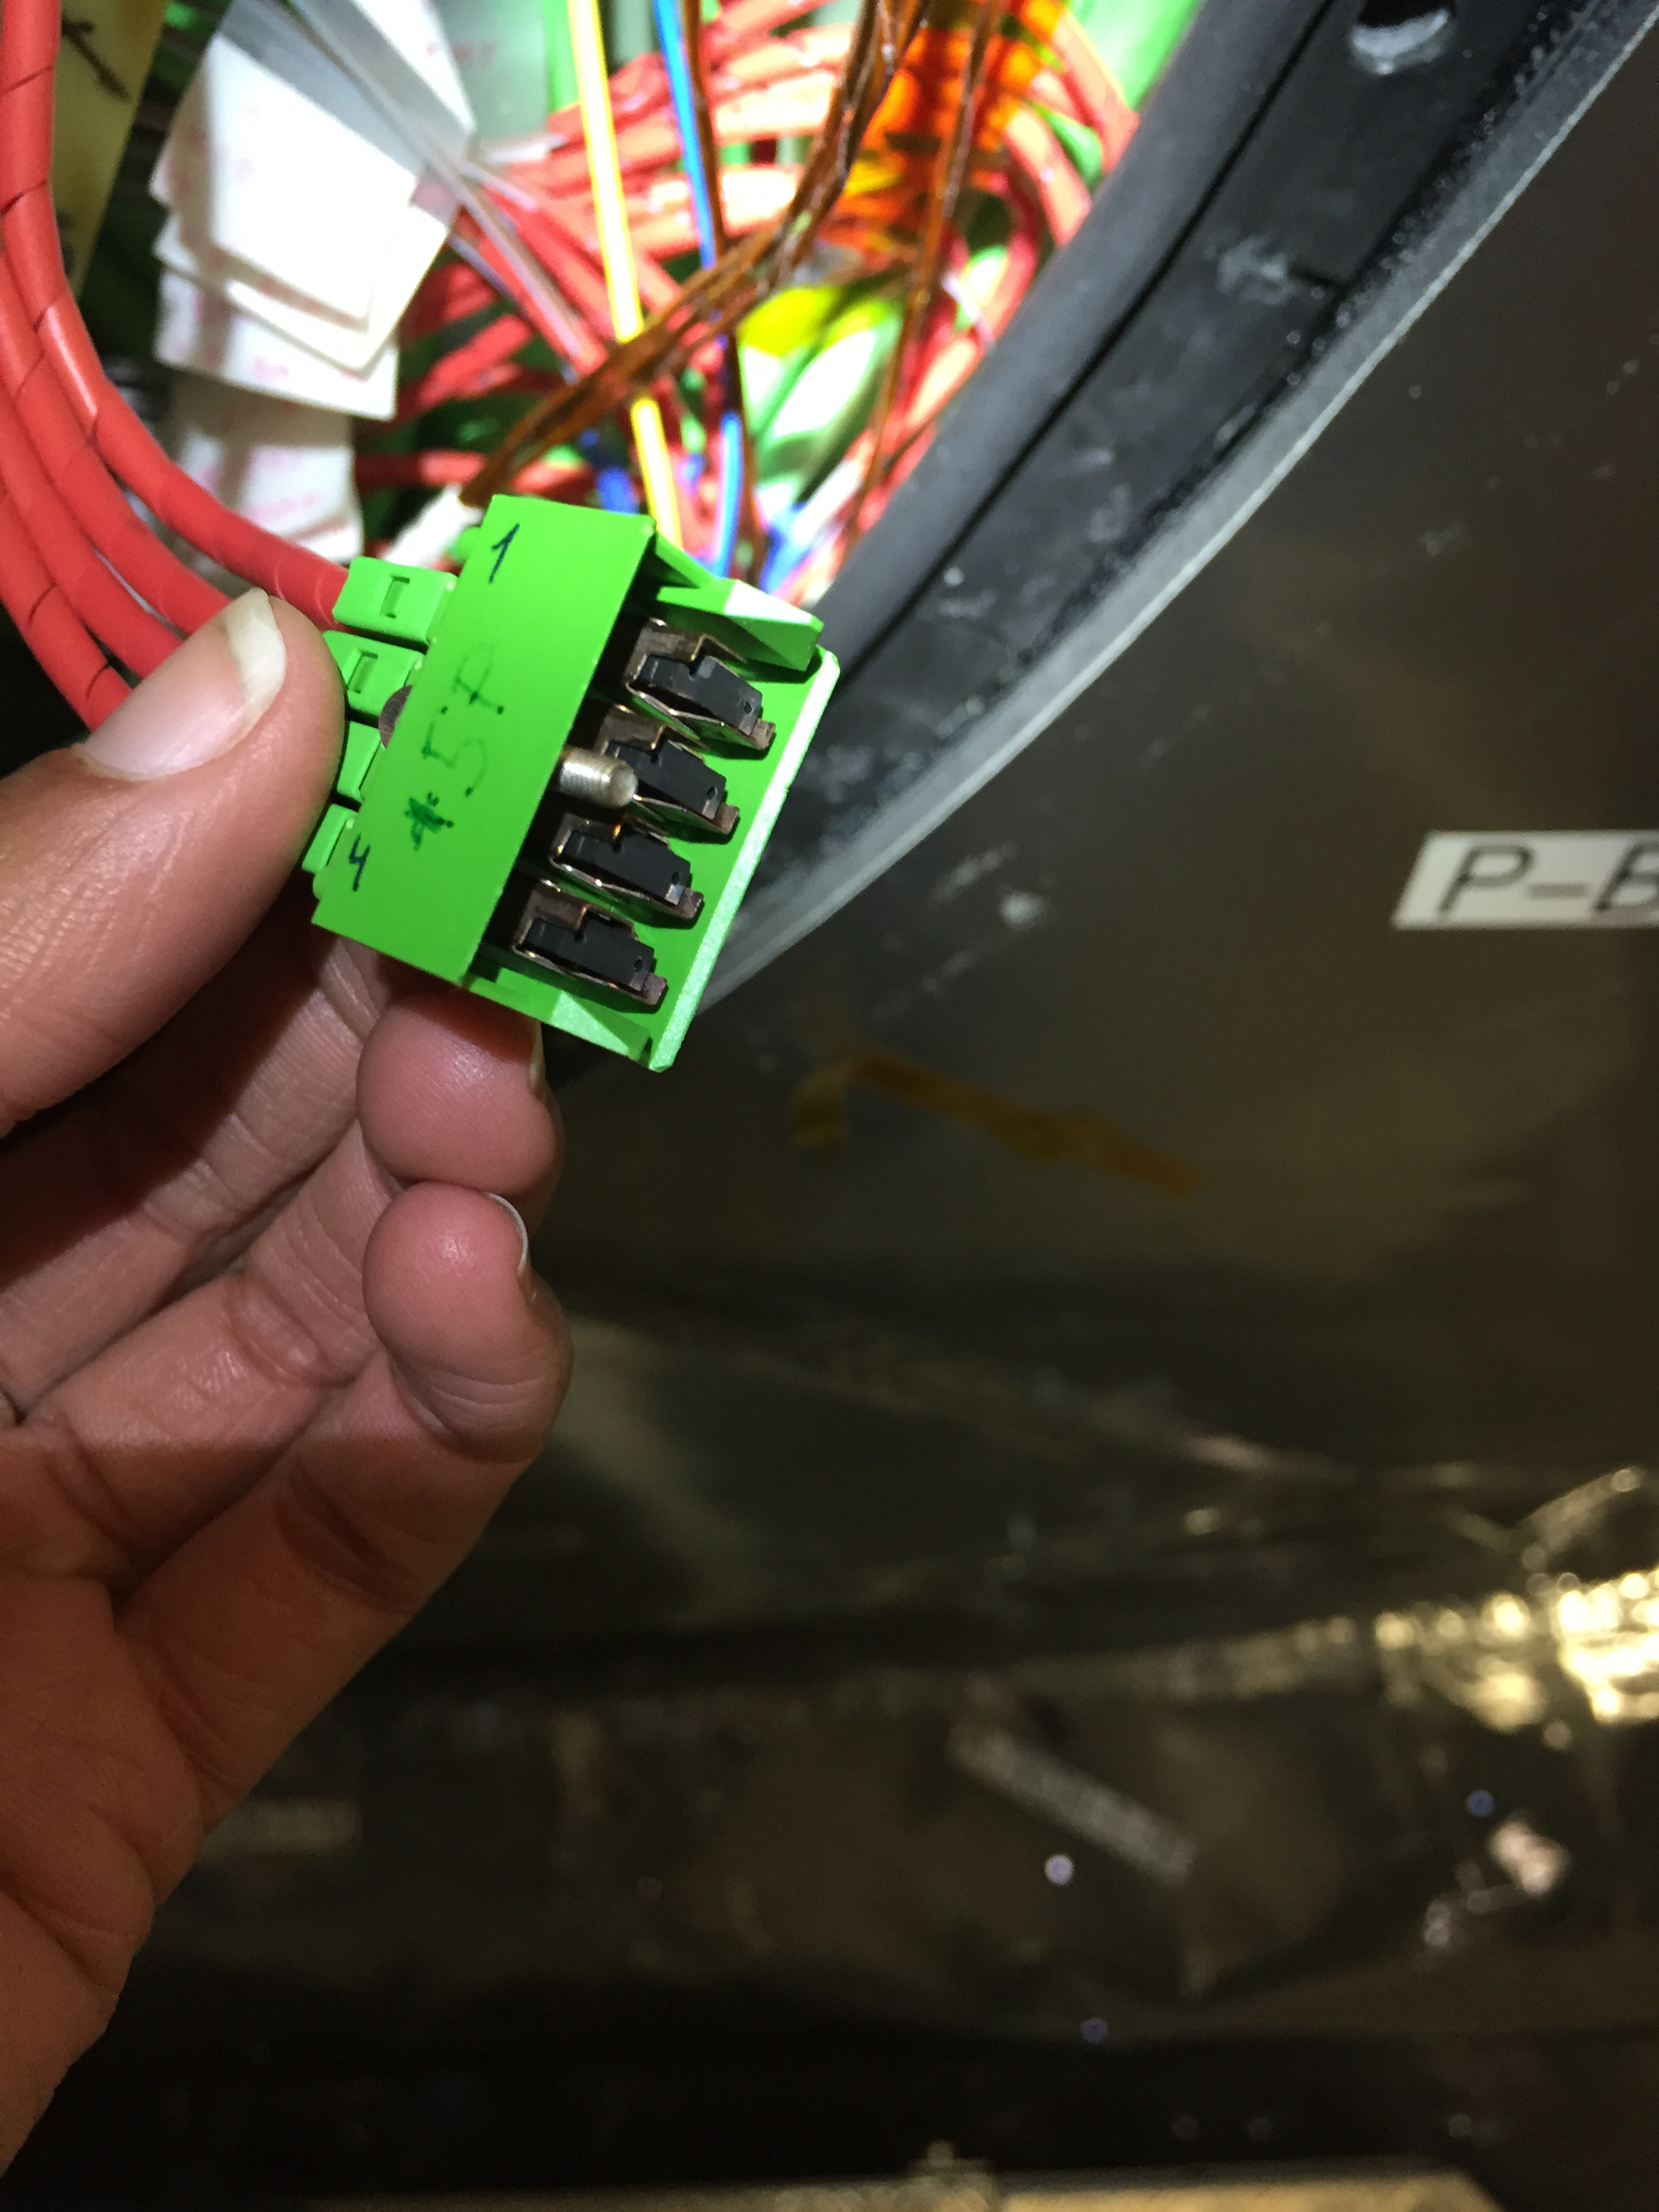
\includegraphics[width=0.3\textwidth]{\chfifteen/OpticalConnector.jpeg}
 %\caption{blabla}
 %\label{fig:OpticalConn}
%\end{wrapfigure}
After the installation, the detector was then checked out at room temperature of about 16\unit{$^\circ$C}.
The basic set of calibrations was run from the CMS control room aimed at assessing the detector status and setting the basic operating parameters.
These include calibrations of the Delay25 chip, FED baseline, AOH bias and gain, TBM and ROC UB, and address levels.
The absence of a good quality TBM signal in the FED (Fig.~\ref{fig:FEDBaseline}) or bad address levels indicate poor optical connections.
This kind of problems were immediately established and solved underground on the platform by re-cleaning the optical connectors with special tools.
Few iterations were needed.
These operations were completed in about 3 days establishing the functionality of the whole BPix detector.
Only 1\% dead or disabled channels were found and most of them were acknowledged during LS1.
The check out procedure was repeated after the insertion of the FPix.

\subsection{Calibrations at -10\unit{$^\circ$C}}\label{sec:FinalBPixCalib}

As discussed at the beginning of this chapter, it was planned to operate the detector at -10\unit{$^\circ$C} since low temperatures
are favorable to mitigate the effects of radiation damage and guarantee excellent performance.
Since the detector settings largely depend on the temperature, a full calibration of the detector under the new conditions has to be performed.
Because of the limited amount of time, it was not possible to achieve this before the re-installation, and tests were conducted for only few sectors aimed at verifying some basic functionalities at such low temperatures.
%However, it was not possible to perform the full calibration at low temperature was never been performed except for the tests conducted in the clean room during LS1
%for only few sectors and aimed at ensuring basic functionalities under such conditions.
The full calibration procedure was instead run in January 2015 and completed in only 8 days, including the final optimization of the signal performance (Section~\ref{subsec:calibPart2}).
The improvements added to the procedure during LS1 as well as the time spent in practicing it 
were crucial to make these time consuming operations much faster and smoother with respect to 2011 and 2012.\\
%The final adjustments of outsiders (ROCs not converging at the end of the procedure) were quite time consuming, typically fixed by hand

The results of the optimization of the signal rise speed are presented in Fig.~\ref{fig:VanaCalib2015}, which shows the 
distributions in DT for all the ROCs at the beginning and at the end of the procedure. A value for the DT of 12 \textit{Vcal} was chosen as a target.
The corresponding average current per ROC measured from the power supplies for each power group are also shown separately for layers 1 and 2 (Fig.~\ref{fig:VanaCalib2015_b}), and layer 3 ((Fig.~\ref{fig:VanaCalib2015_c})).

\begin{figure}[!htb]
 \begin{center}
 \subfigure[]{\label{fig:VanaCalib2015_a}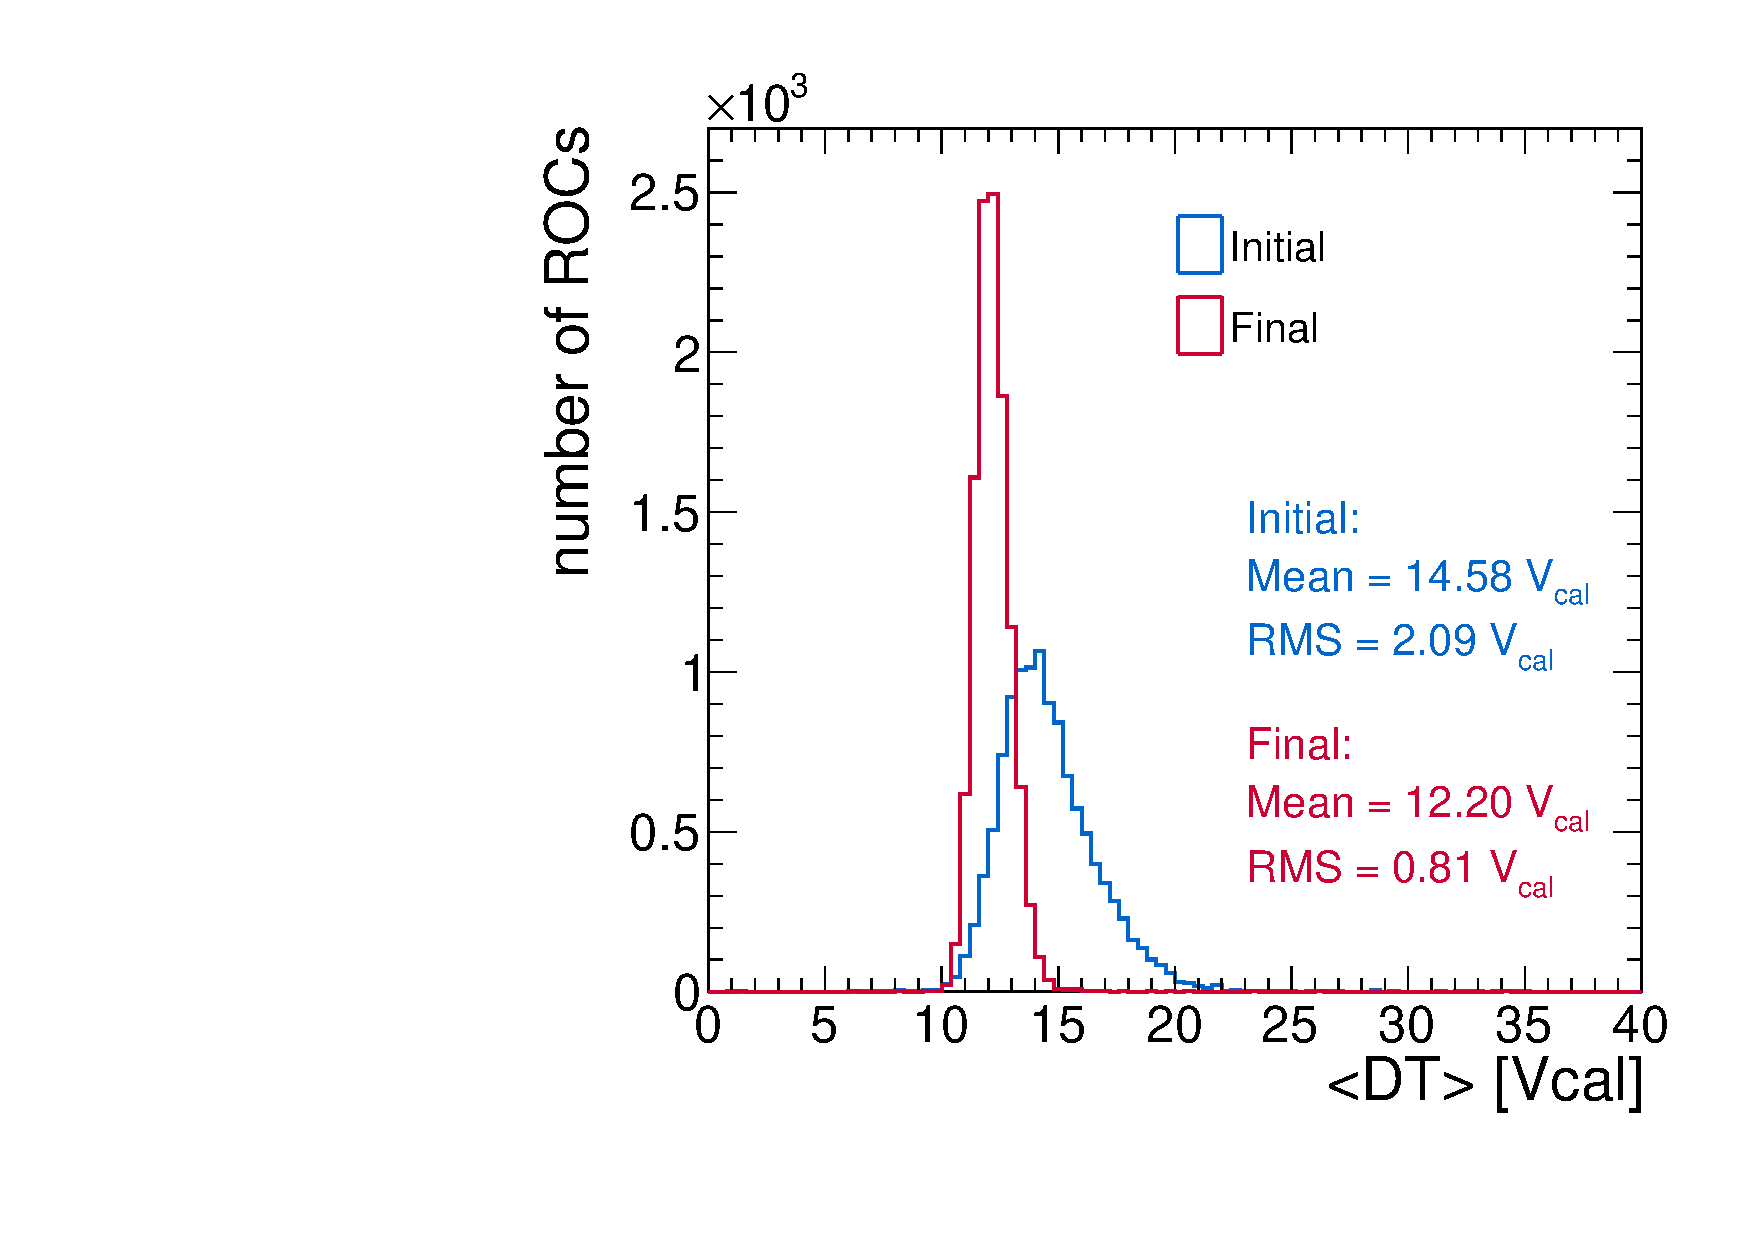
\includegraphics[width=0.3\textwidth]{\chfifteen/DT-2015.pdf}}
 \subfigure[]{\label{fig:VanaCalib2015_b}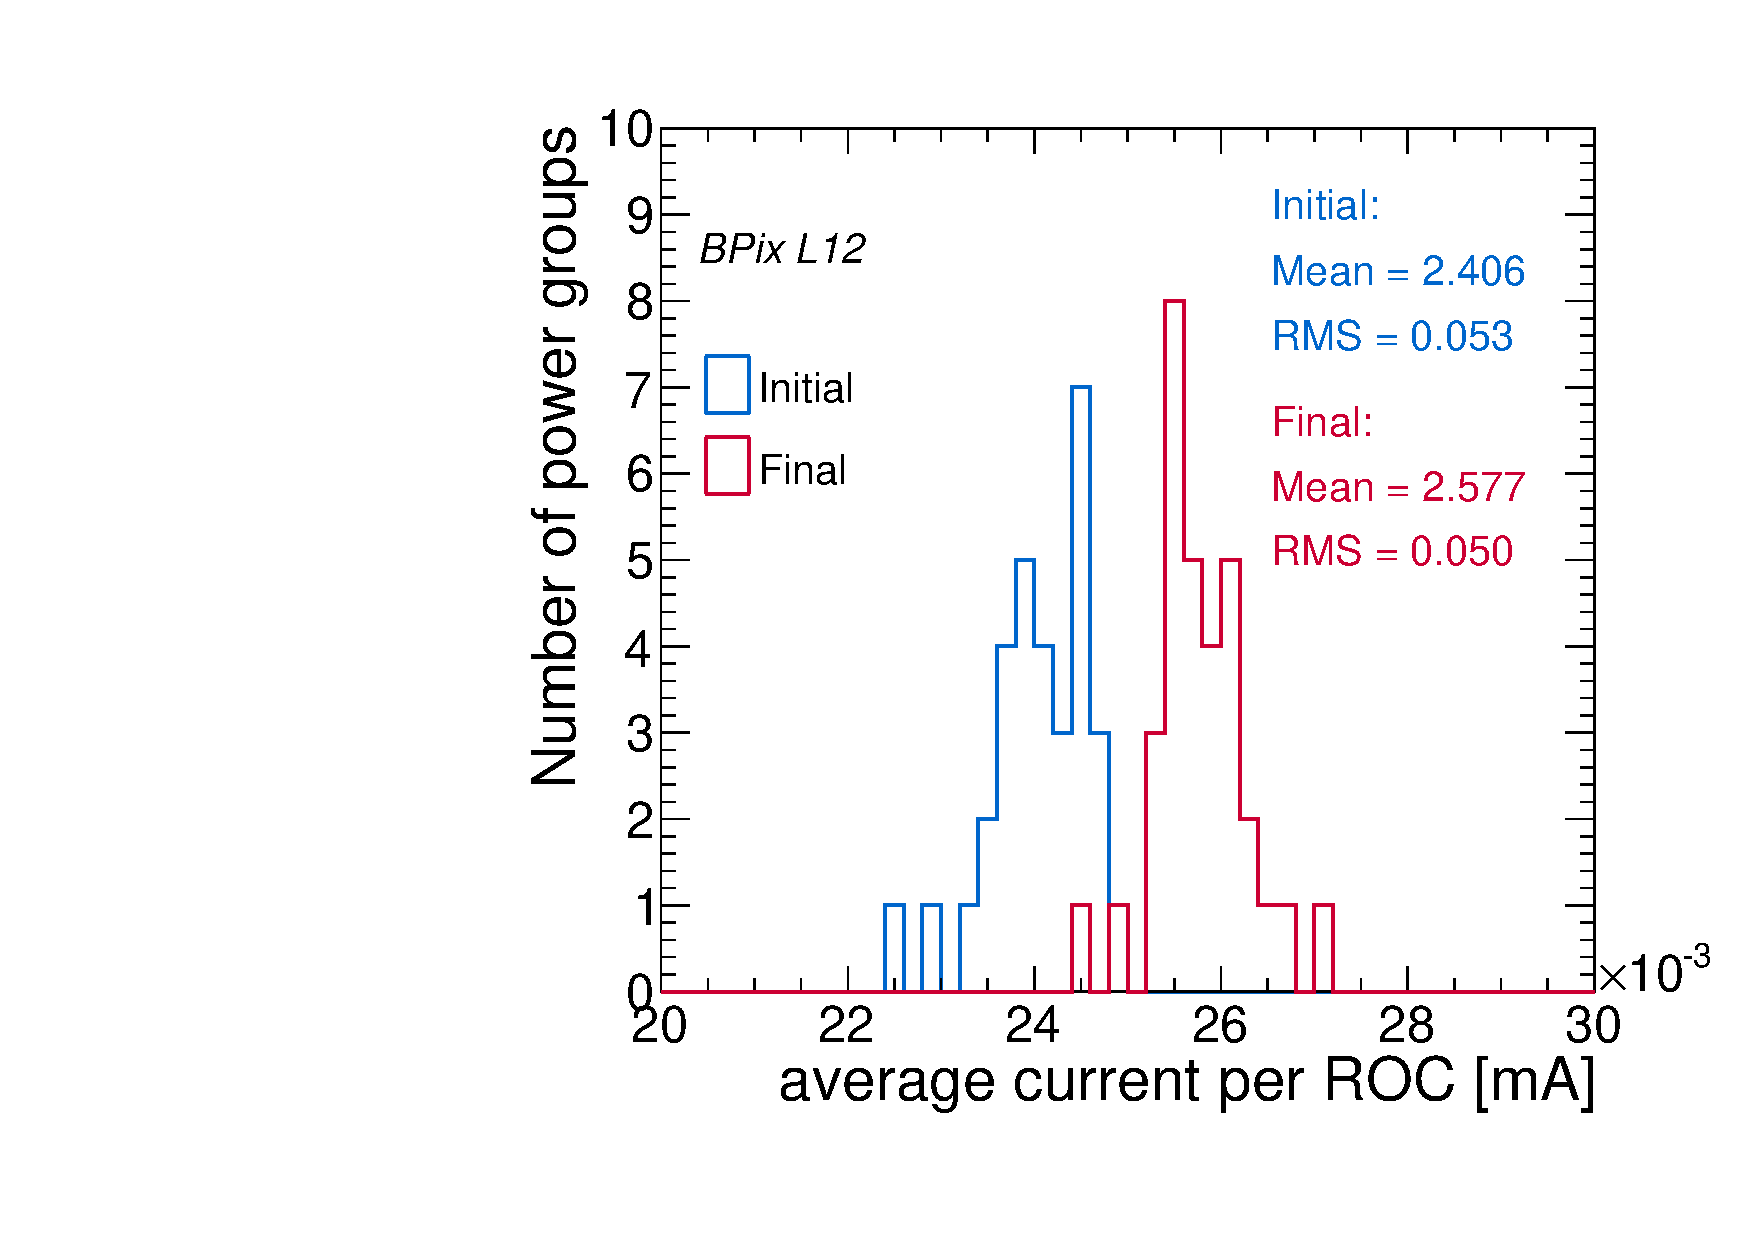
\includegraphics[width=0.3\textwidth]{\chfifteen/Iana-2015-L12.pdf}}
 \subfigure[]{\label{fig:VanaCalib2015_c}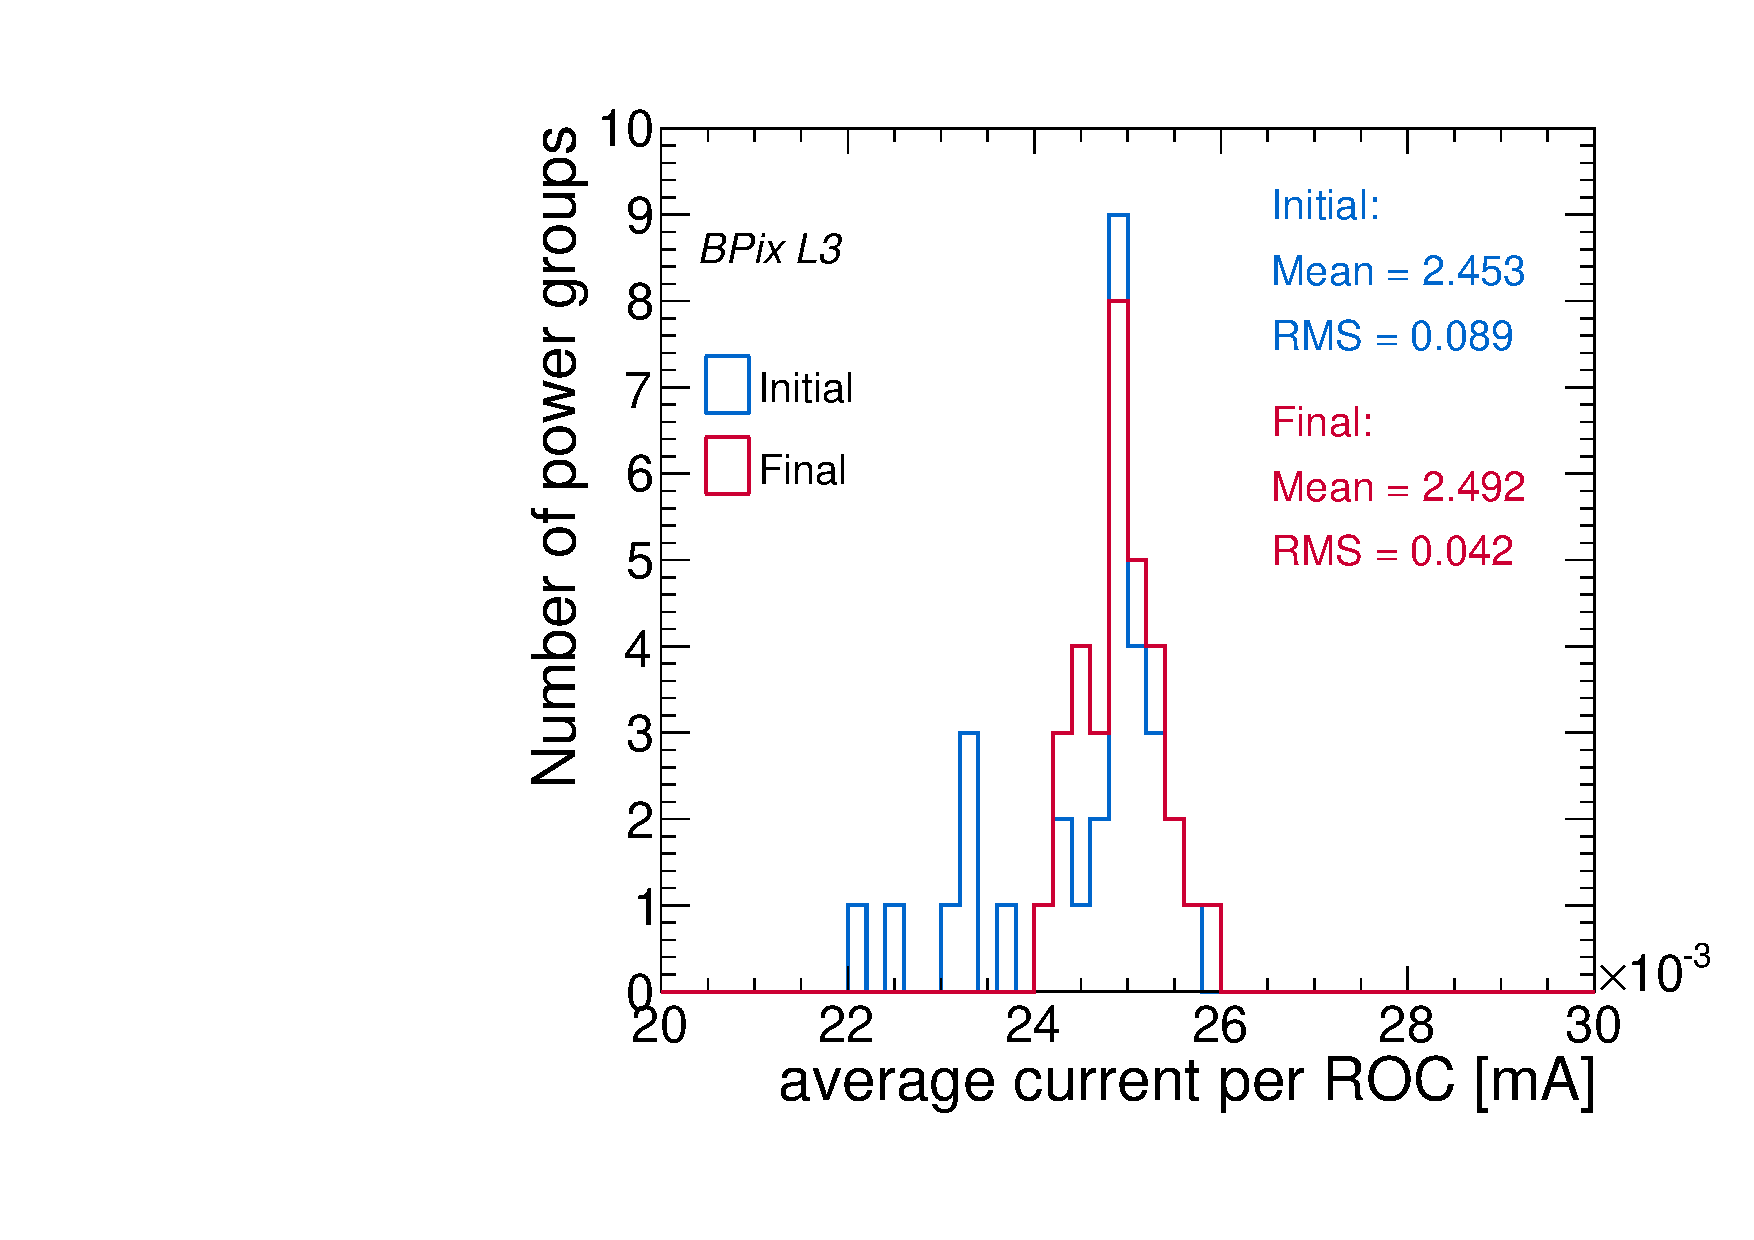
\includegraphics[width=0.3\textwidth]{\chfifteen/Iana-2015-L3.pdf}}
 \end{center}
 \caption{(a) Distributions in DT at the beginning and end of the optimization of the signal rise speed performed in 2015 for BPix Run~2 commissioning. (b-c) Corresponding average analog current per ROC after reaching the target DT value of 12 \textit{Vcal}.}
 \label{fig:VanaCalib2015}
\end{figure}

Figure~\ref{fig:ThrCalib2015} shows the final threshold and noise distributions for all pixels obtained after the procedure of minimization described in Section~\ref{subsec:calibPart2}.
%The results of the optimization of the pixel threshold are presented in Fig.~\ref{fig:ThrCalib2015} that shows the final average threshold and noise per ROC in \textit{Vcal} units.
The spread of the thresholds in each ROC is also shown, quantified by the RMS of the individual ROC distributions.
A final average threshold of $\approx$ 40 \textit{Vcal} (2,200 electrons) was obtained showing agreement with the results of the tests performed in the clean room (Fig.~\ref{fig:ThrCalibLS1})
and with the Run~1 values (Fig.~\ref{fig:PixRadDamag}).
Finally, the measured distributions of the gain and pedestal for each pixel used for the offline reconstruction of clusters are presented in Fig.~\ref{fig:GainCalib2015}.
The distribution of the linearity parameter of the response curve as extracted from the fits is also shown.
%The gain distribution has a mean at 2.5 and an RMS of about 0.4. The offset distribution has a mean at 55 ADC units (12700 electrons) and an RMS of 12.

\begin{figure}[!htb]
 \begin{center}
 \subfigure[]{\label{fig:ThrCalib2015_a}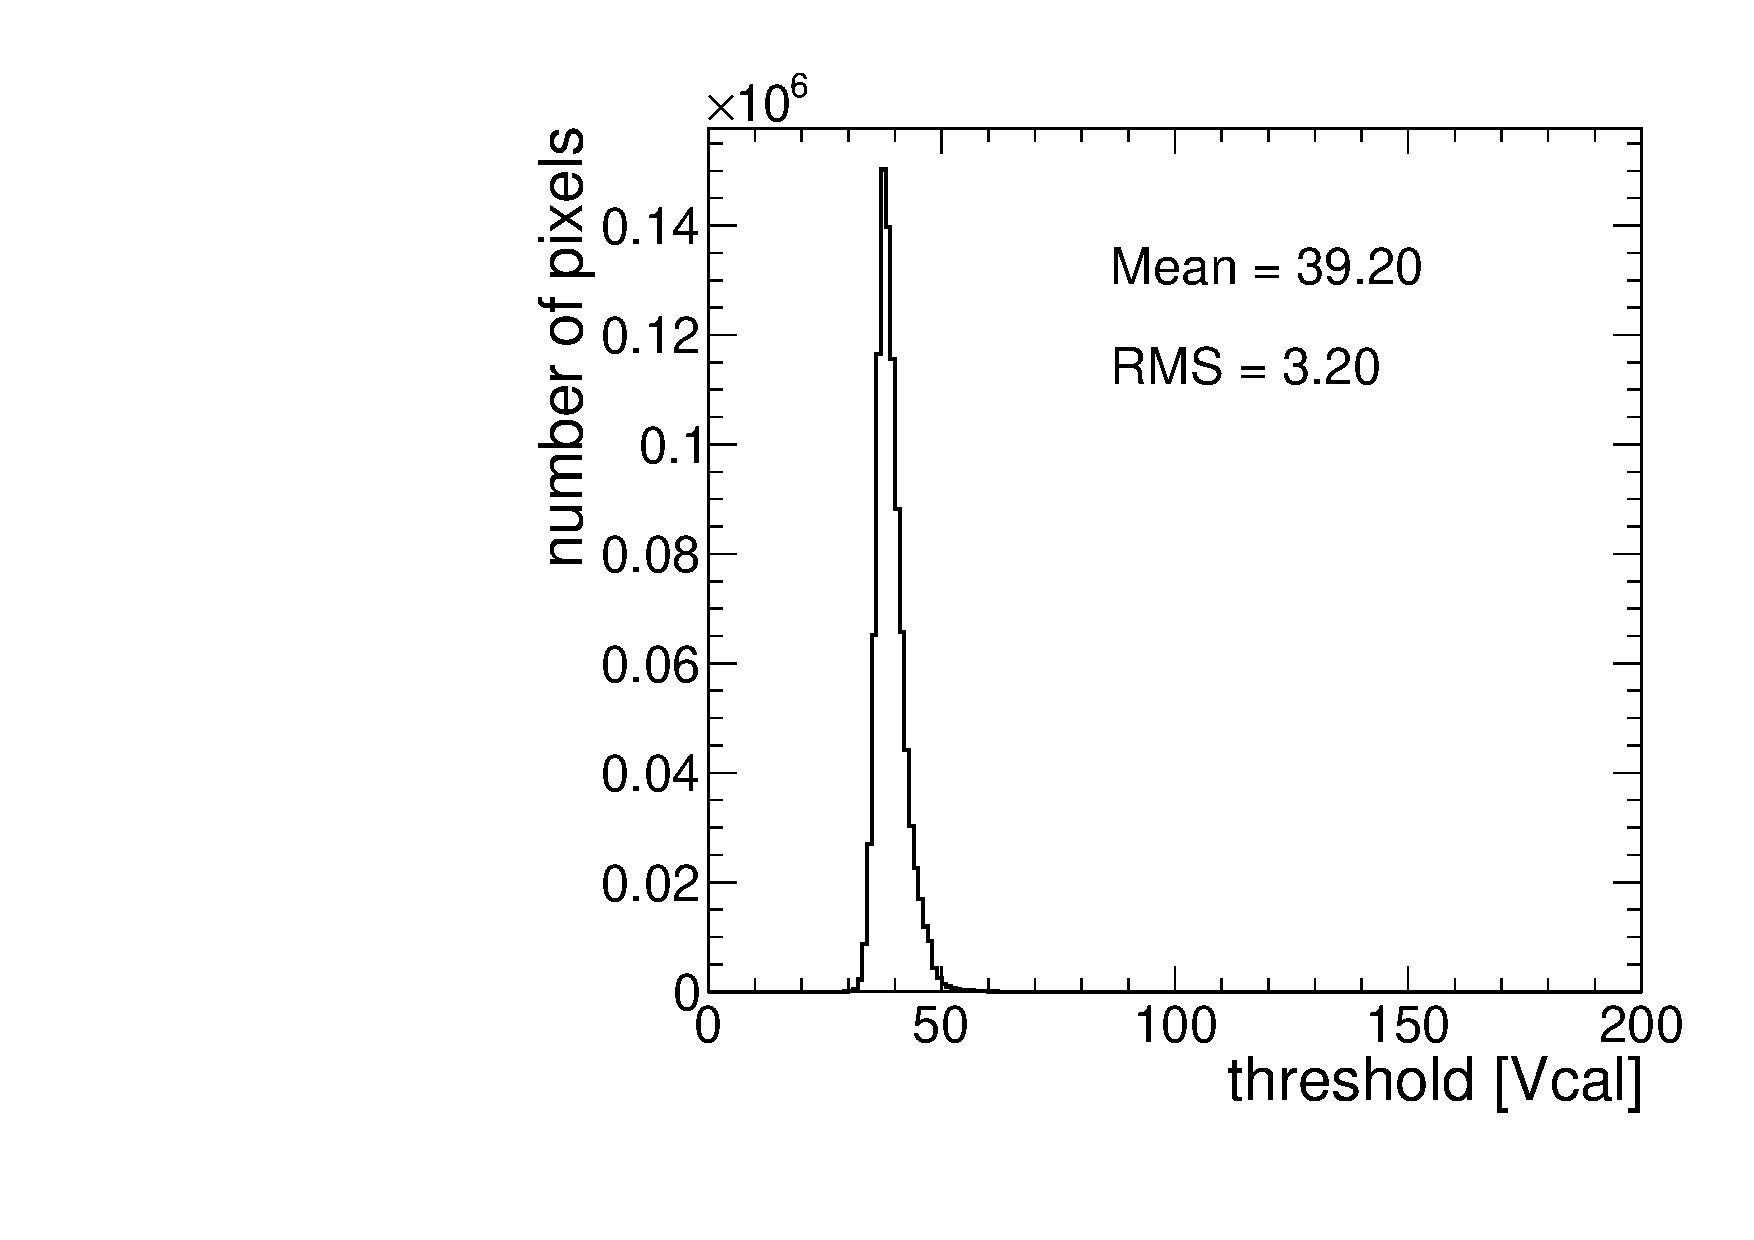
\includegraphics[width=0.3\textwidth]{\chfifteen/threshold-2015-allpixels.pdf}}
 \subfigure[]{\label{fig:ThrCalib2015_b}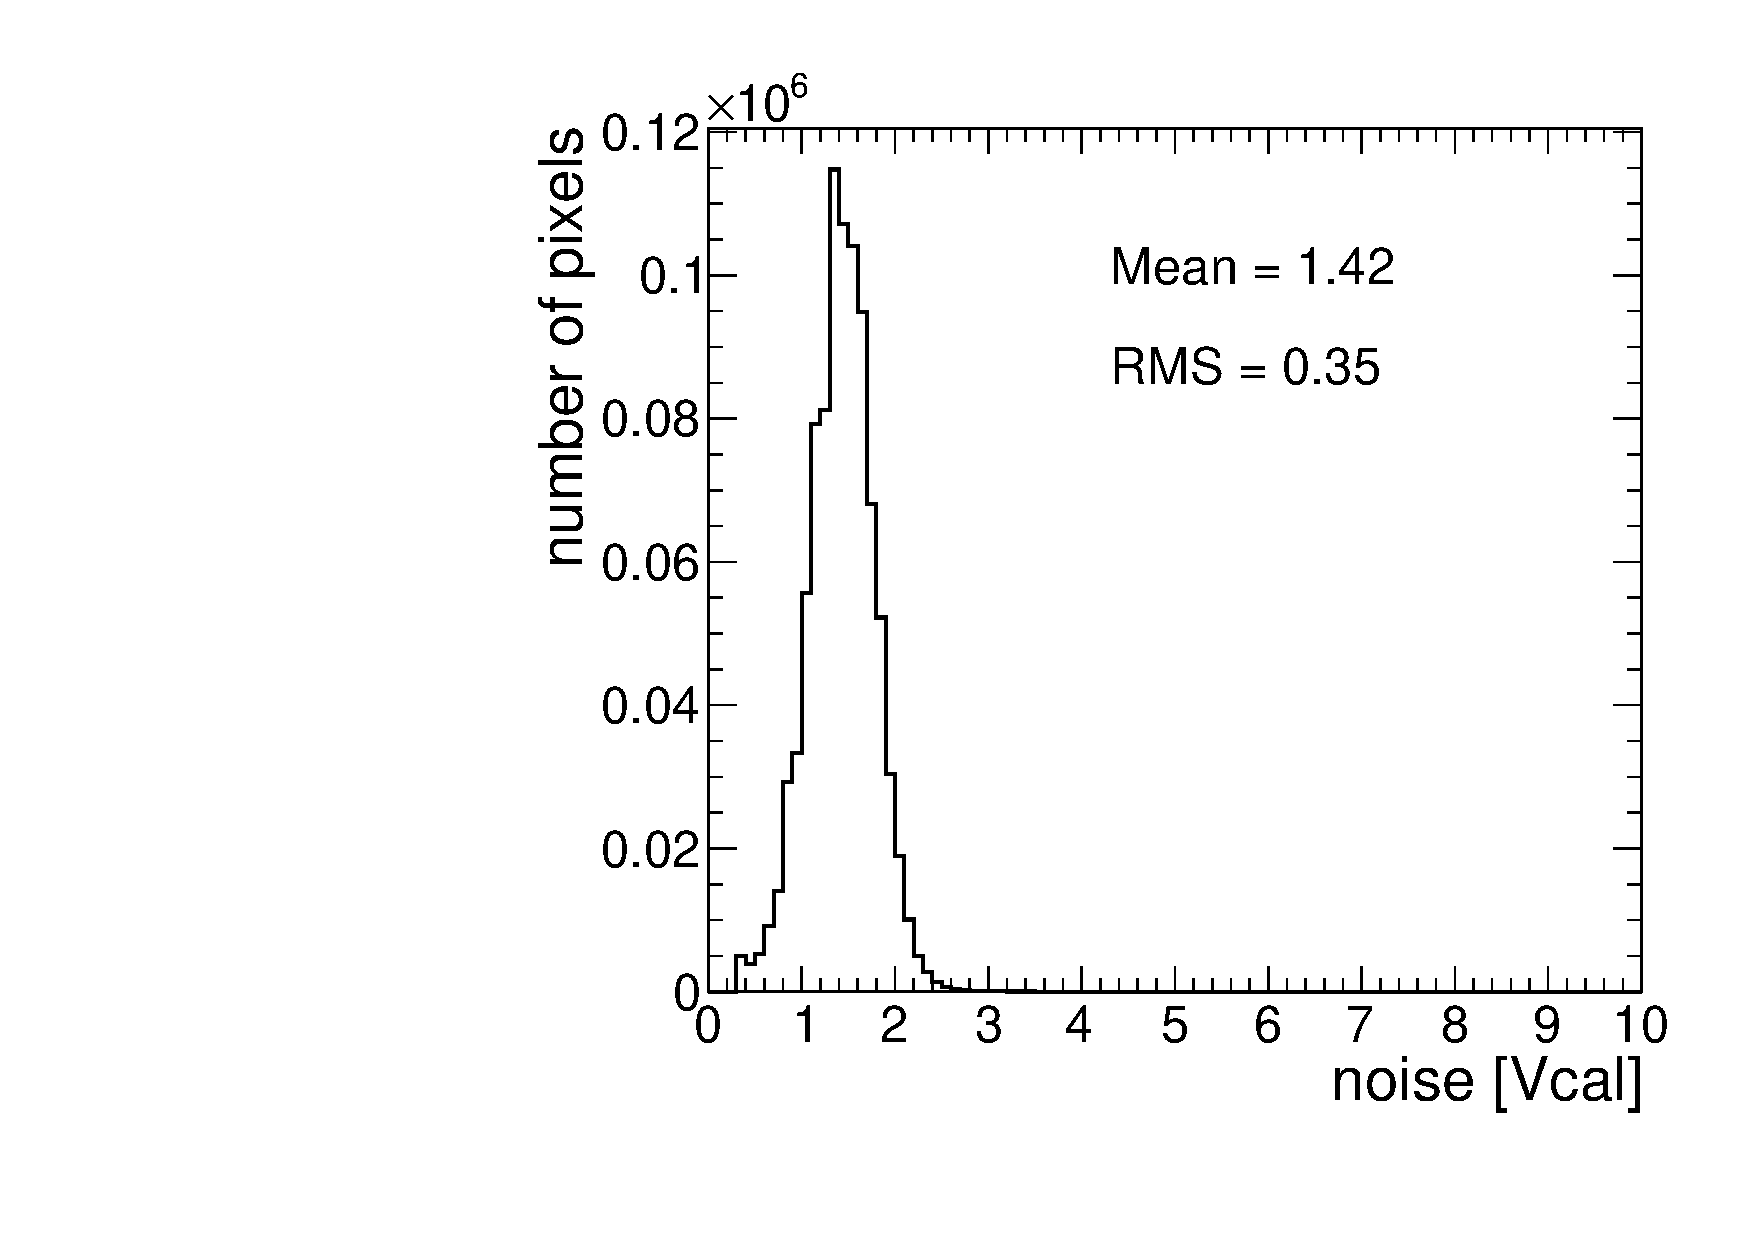
\includegraphics[width=0.3\textwidth]{\chfifteen/noise-2015-allpixels.pdf}}
 \subfigure[]{\label{fig:ThrCalib2015_c}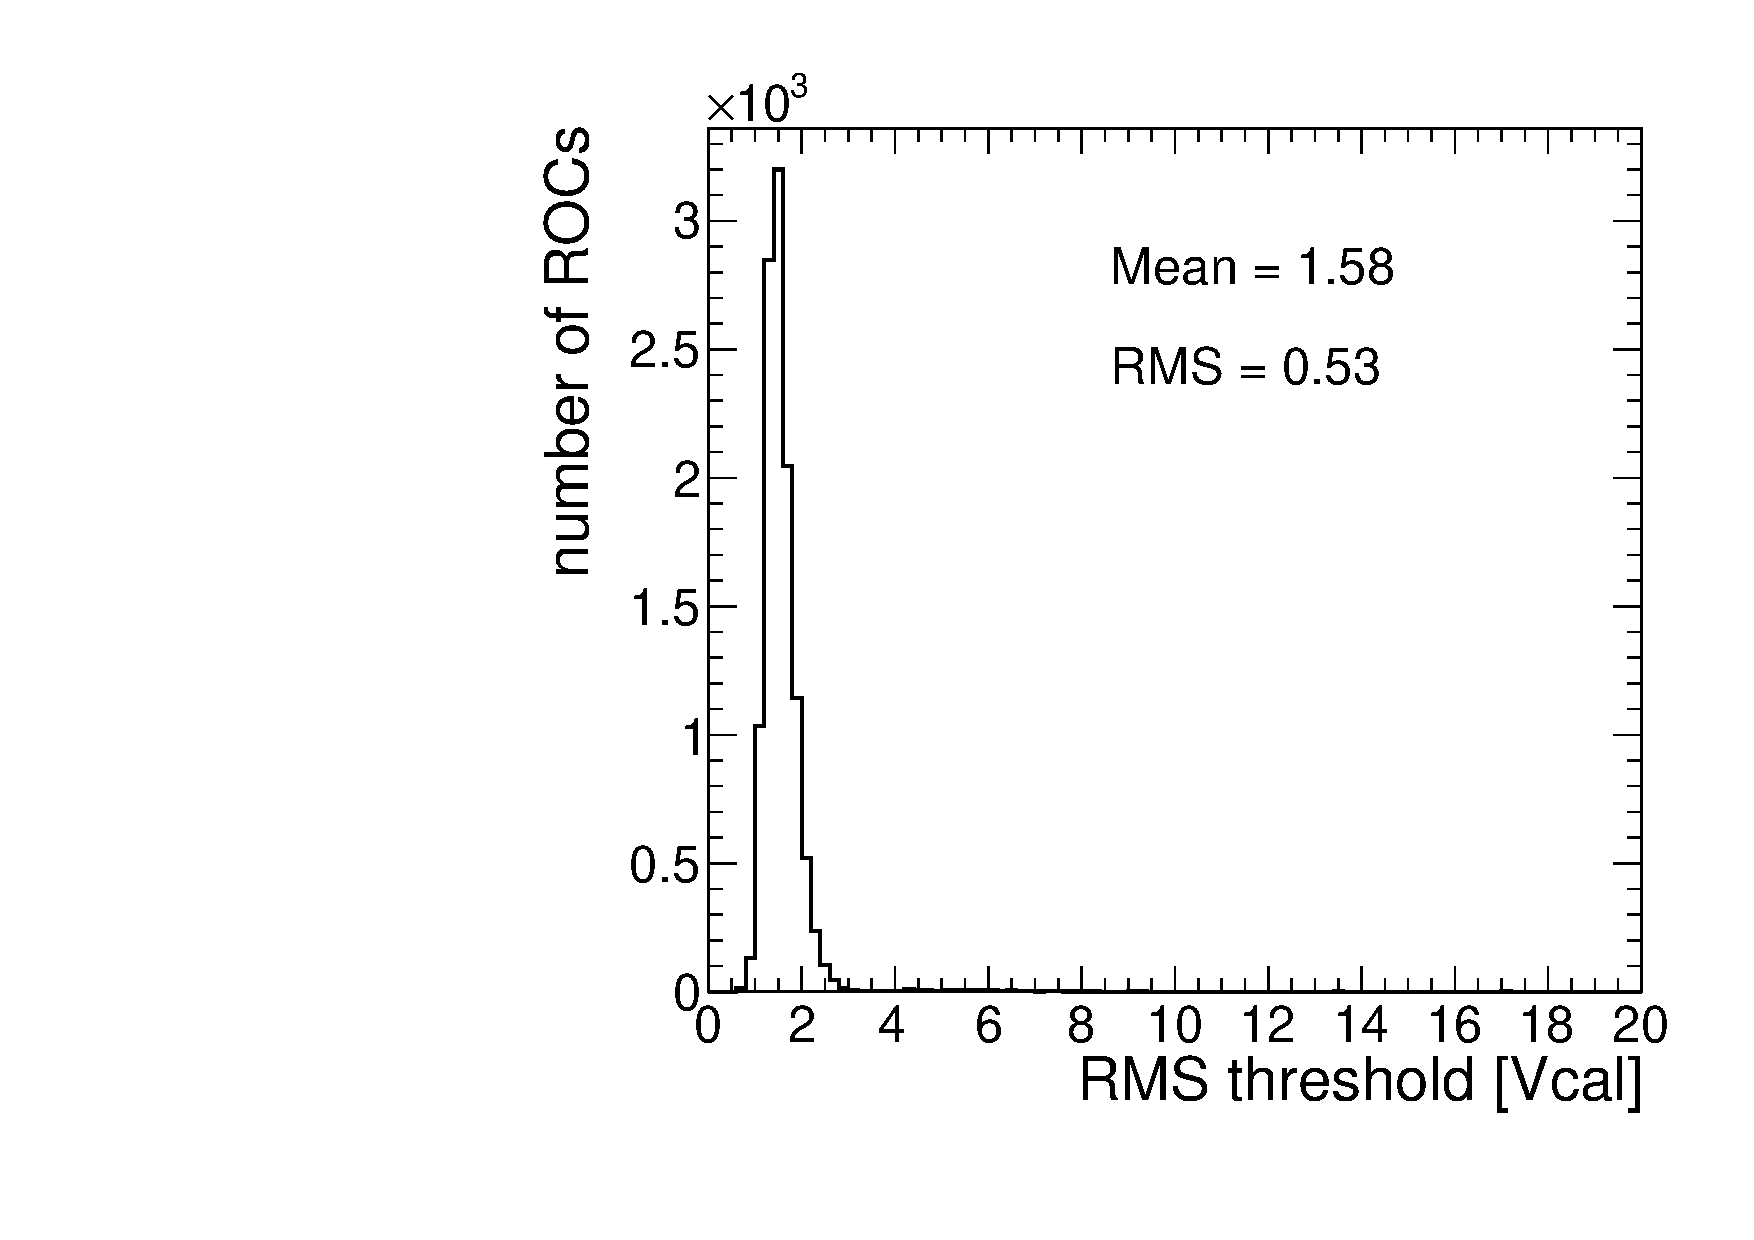
\includegraphics[width=0.3\textwidth]{\chfifteen/rmsthreshold-2015-my.pdf}}
 \end{center}
 \caption{(a) Threshold and (b) noise distribution for pixels after the calibrations performed in 2015 for Run~2 commissioning. (c) The RMS of the threshold distributions within single ROCs quantifying its spread among cells. All distributions are in units of \textit{Vcal} (1 \textit{Vcal} = 65.5 electrons).}
 \label{fig:ThrCalib2015}
\end{figure}

\begin{figure}[!htb]
 \begin{center}
 \subfigure[]{\label{fig:GainCalib2015_a}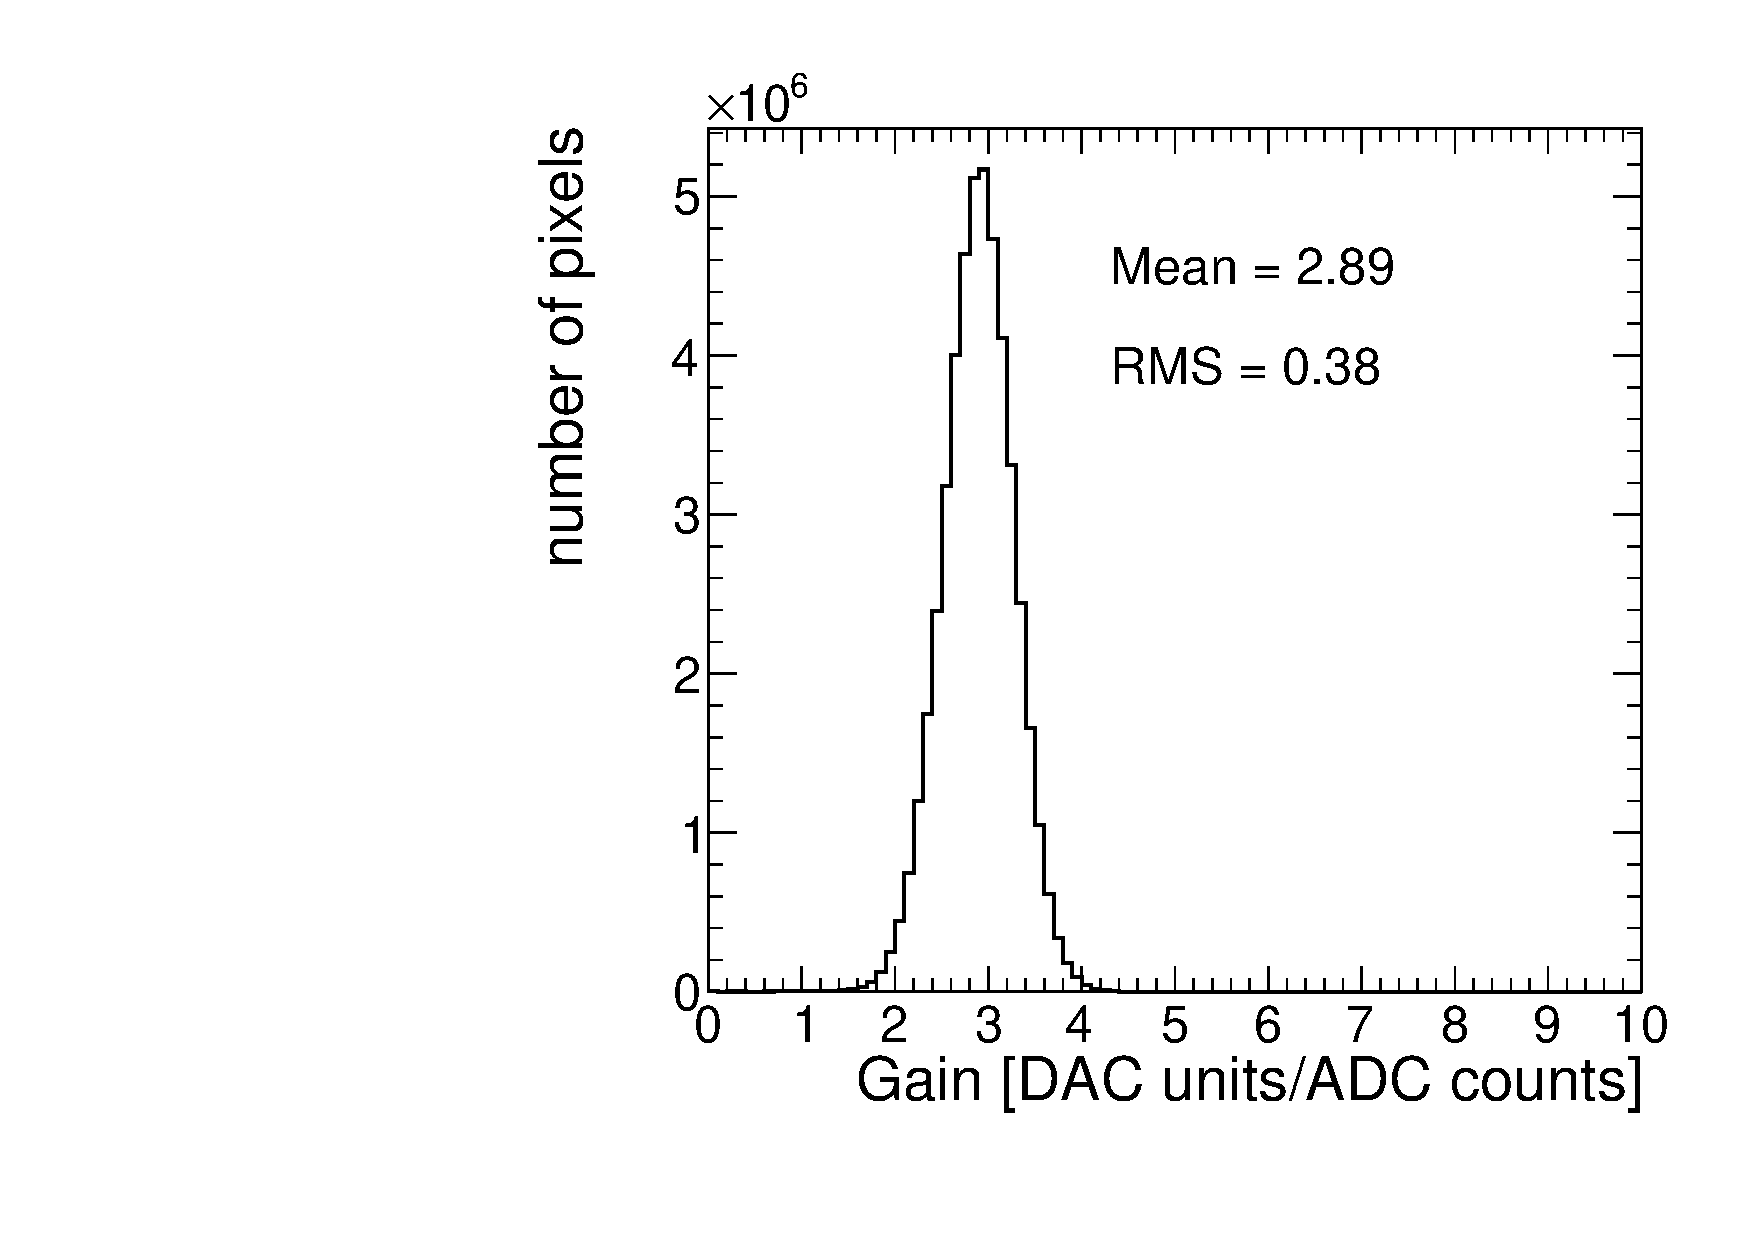
\includegraphics[width=0.3\textwidth]{\chfifteen/gain-2015-my.pdf}}
 \subfigure[]{\label{fig:GainCalib2015_b}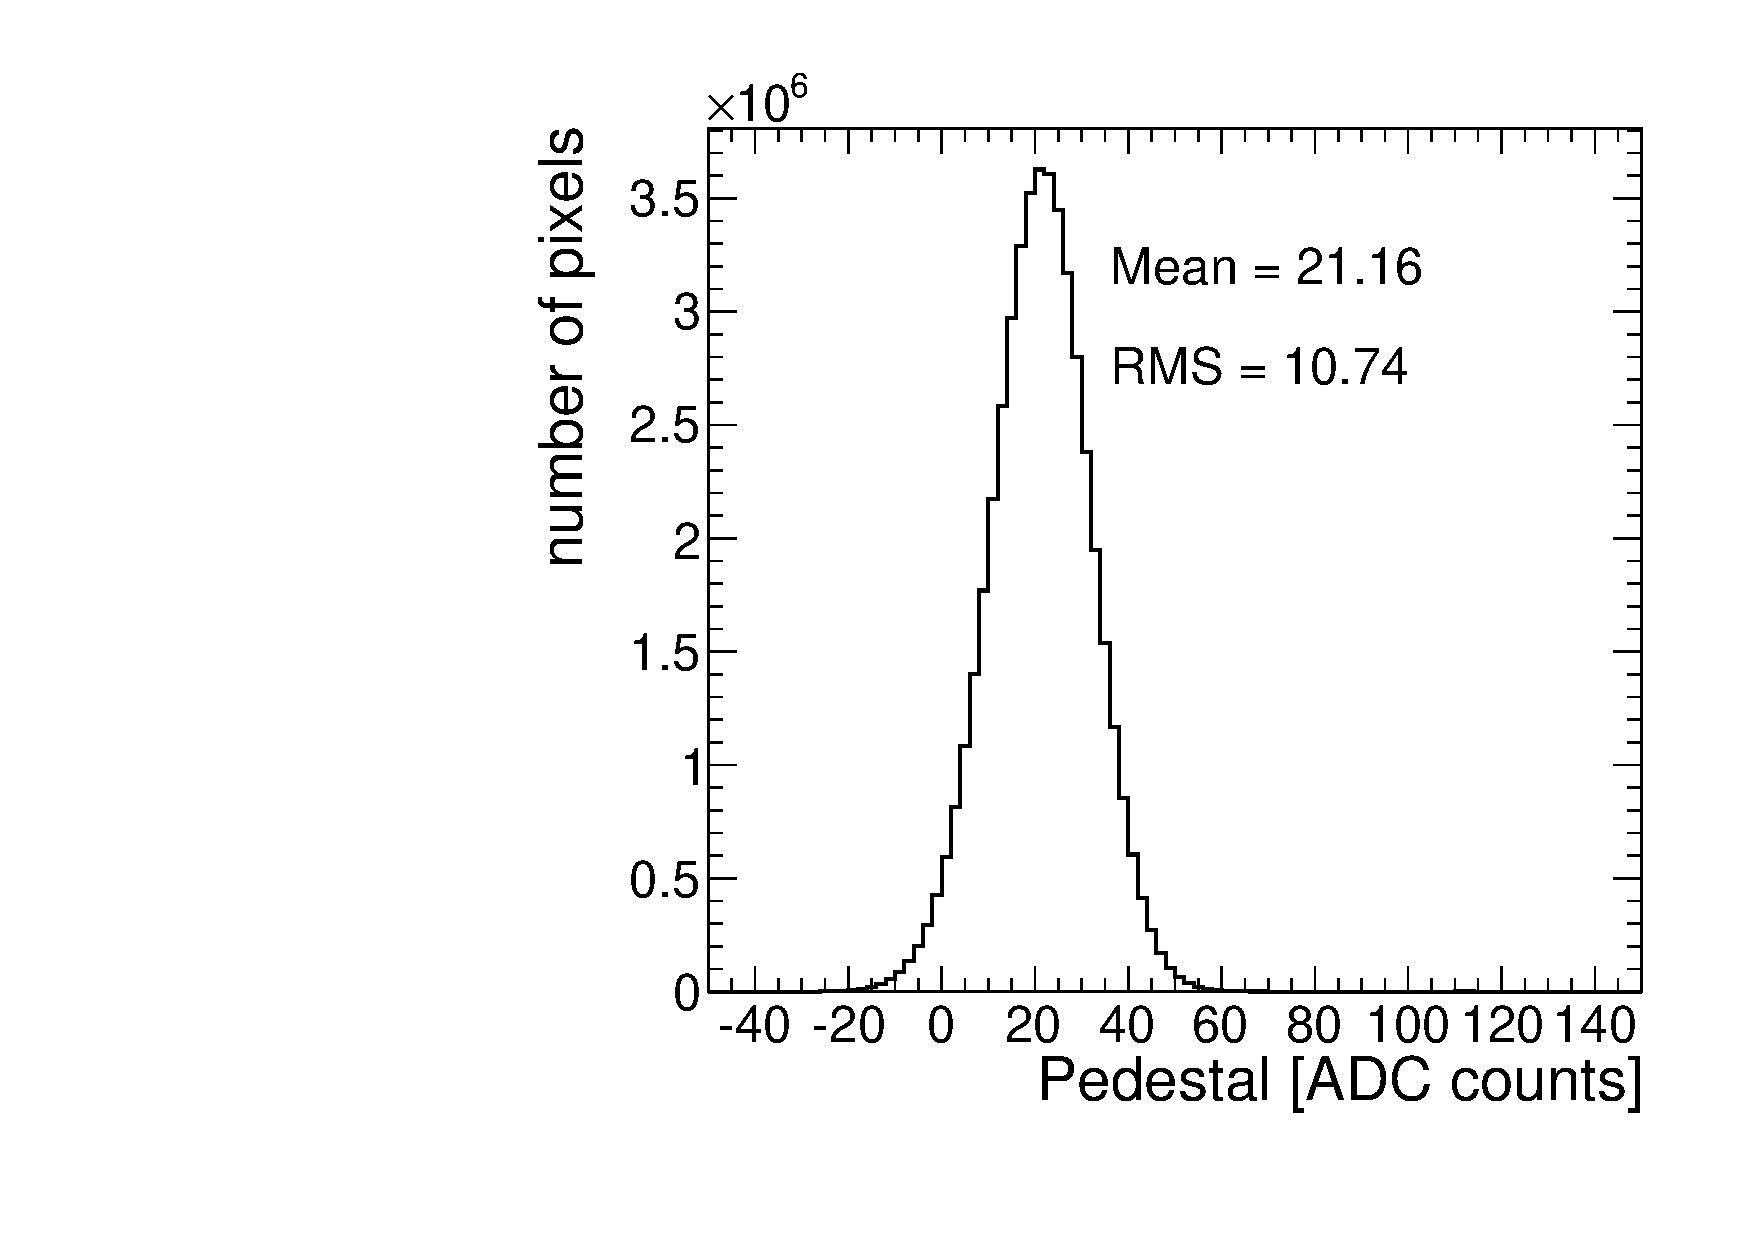
\includegraphics[width=0.3\textwidth]{\chfifteen/pedestal-2015-my.pdf}}
 \subfigure[]{\label{fig:GainCalib2015_c}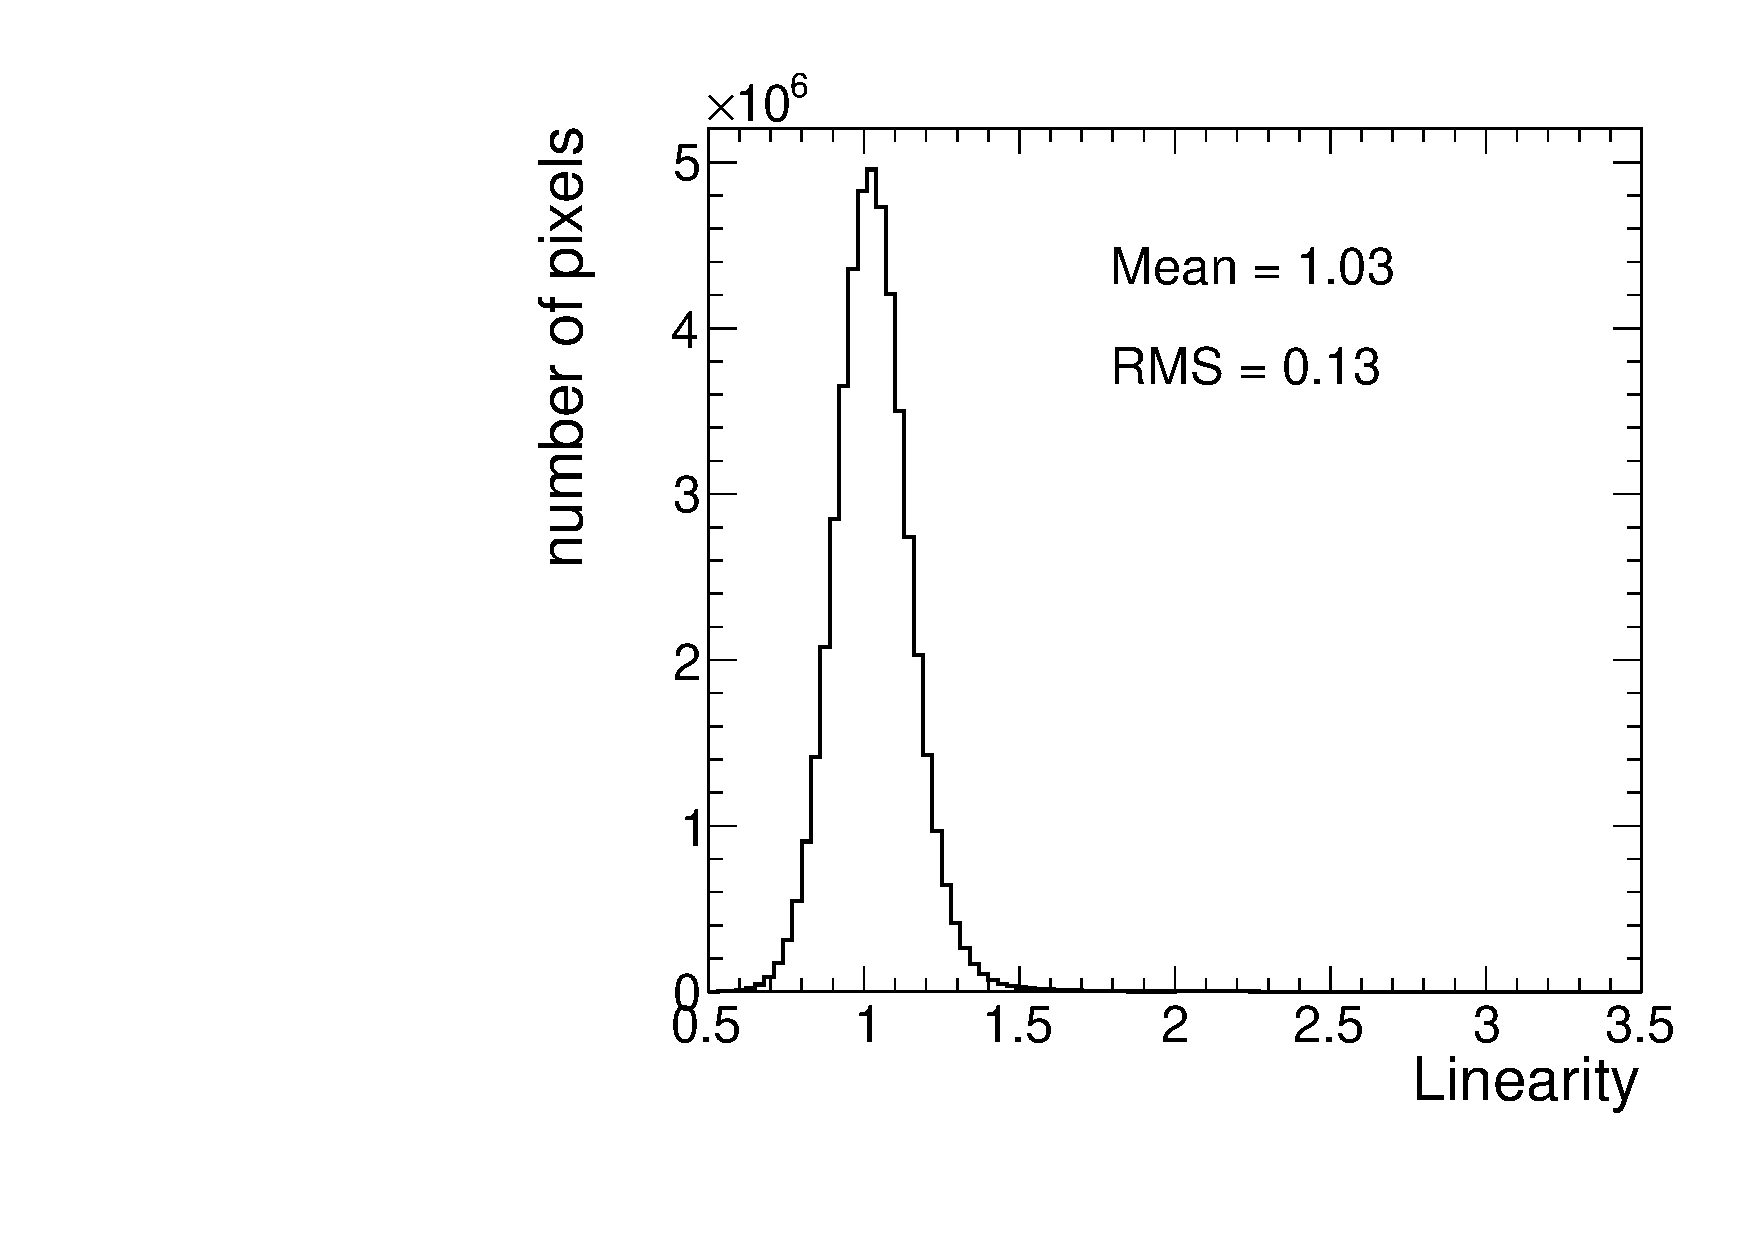
\includegraphics[width=0.3\textwidth]{\chfifteen/linearity-2015-my.pdf}}
 \end{center}
 \caption{Gain (a) and pedestal (b) distributions extracted from the linear fits to the gain response curves of all pixels. These parameters are used for the offline reconstruction of clusters. (c) Distribution of the linearity parameter of the response curve as extracted from the fit.}
 \label{fig:GainCalib2015}
\end{figure}

%results of gain calibration
%results with cosmic

%%%%%%%%%%%%%%%%%%%%%
\section{Performance at the start of Run 2}\label{sec:BPixPerf2015}
%%%%%%%%%%%%%%%%%%%%%

The detector re-calibration discussed in the previous section has been crucial to ensure excellent performance during the start-up of data-taking in 2015.
Figure~\ref{fig:ThrVsLumi2015} shows the average threshold, RMS and noise in units of 1 ke for each barrel pixel layer as a function of the integrated luminosity delivered in 2015.
Due to the different levels of irradiation, the old and new modules have been monitored separately.
The threshold of the new modules rapidly increased with irradiation as was observed also in Run~1 (Fig.~\ref{fig:PixRadDamag}).
The noise quickly reached similar values as that of the old modules, which no longer experience such large changes due to irradiation.

\begin{figure}[!htb]
 \begin{center}
 \subfigure[]{\label{fig:ThrVsLumi2015_a}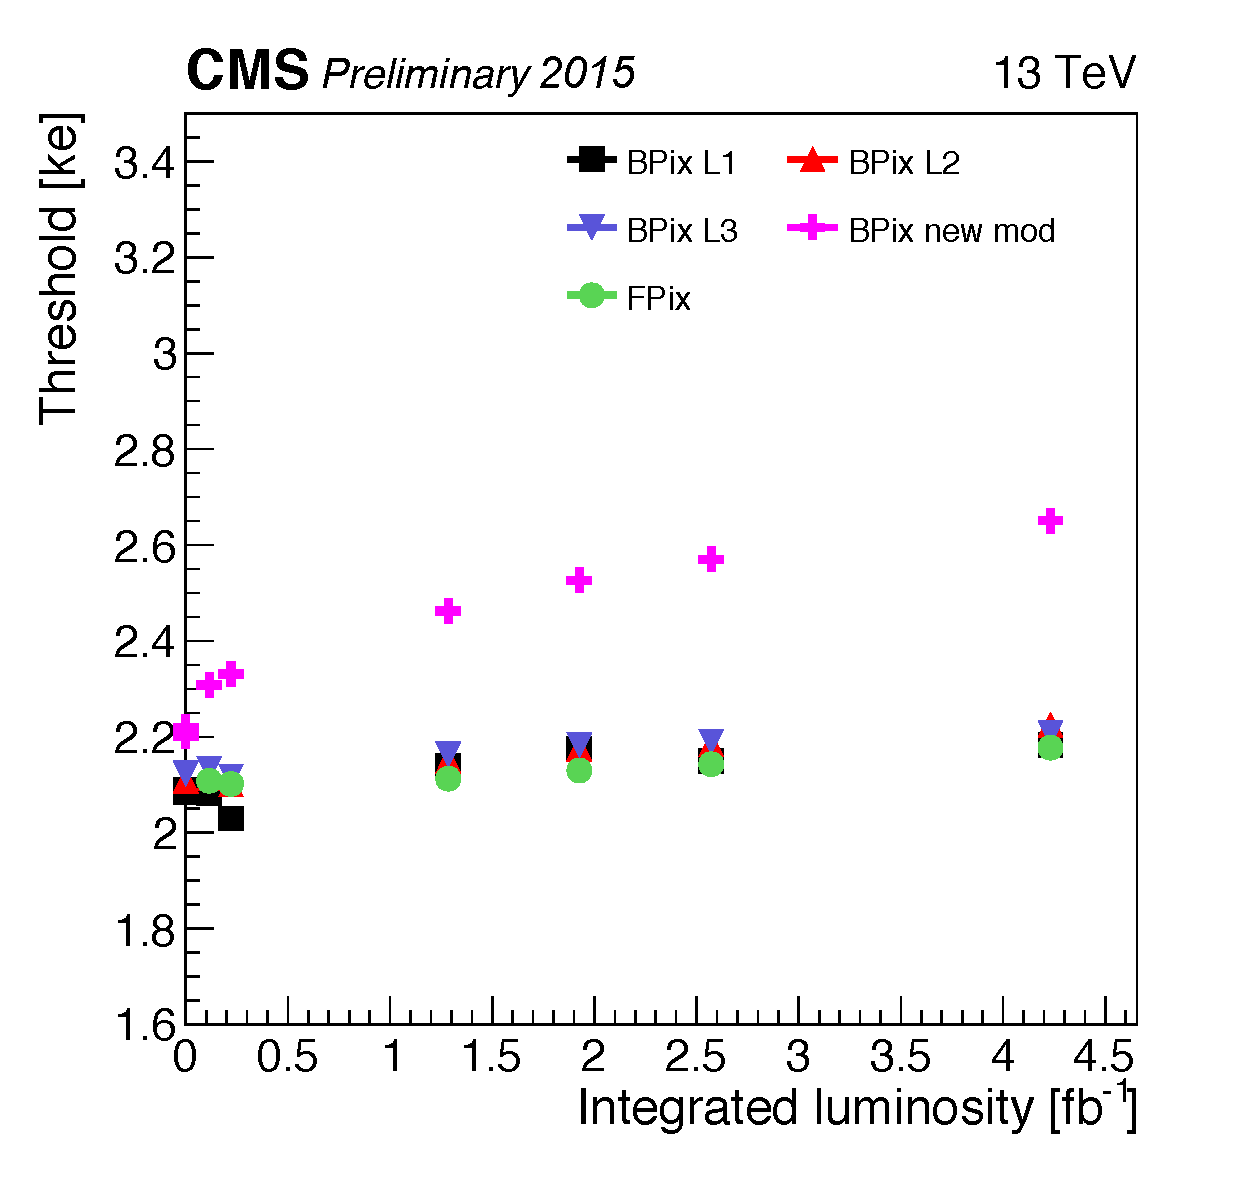
\includegraphics[width=0.3\textwidth]{\chfifteen/thrwbc2bpix_fpix.pdf}}
 \subfigure[]{\label{fig:ThrVsLumi2015_b}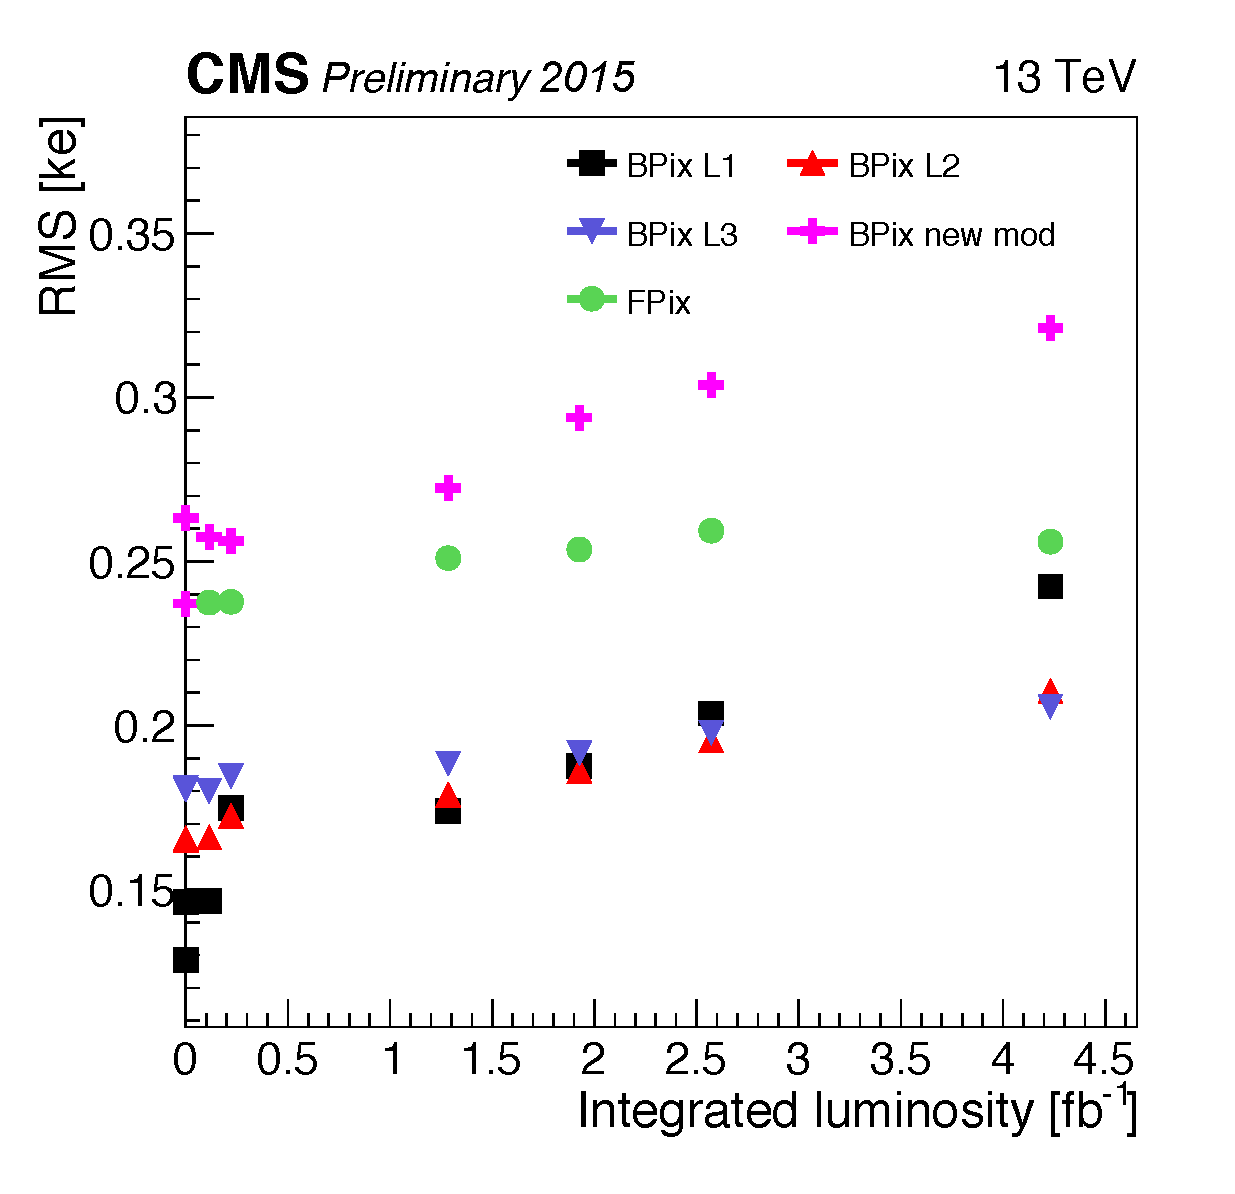
\includegraphics[width=0.3\textwidth]{\chfifteen/rmswbc2bpix_fpix.pdf}}
 \subfigure[]{\label{fig:ThrVsLumi2015_c}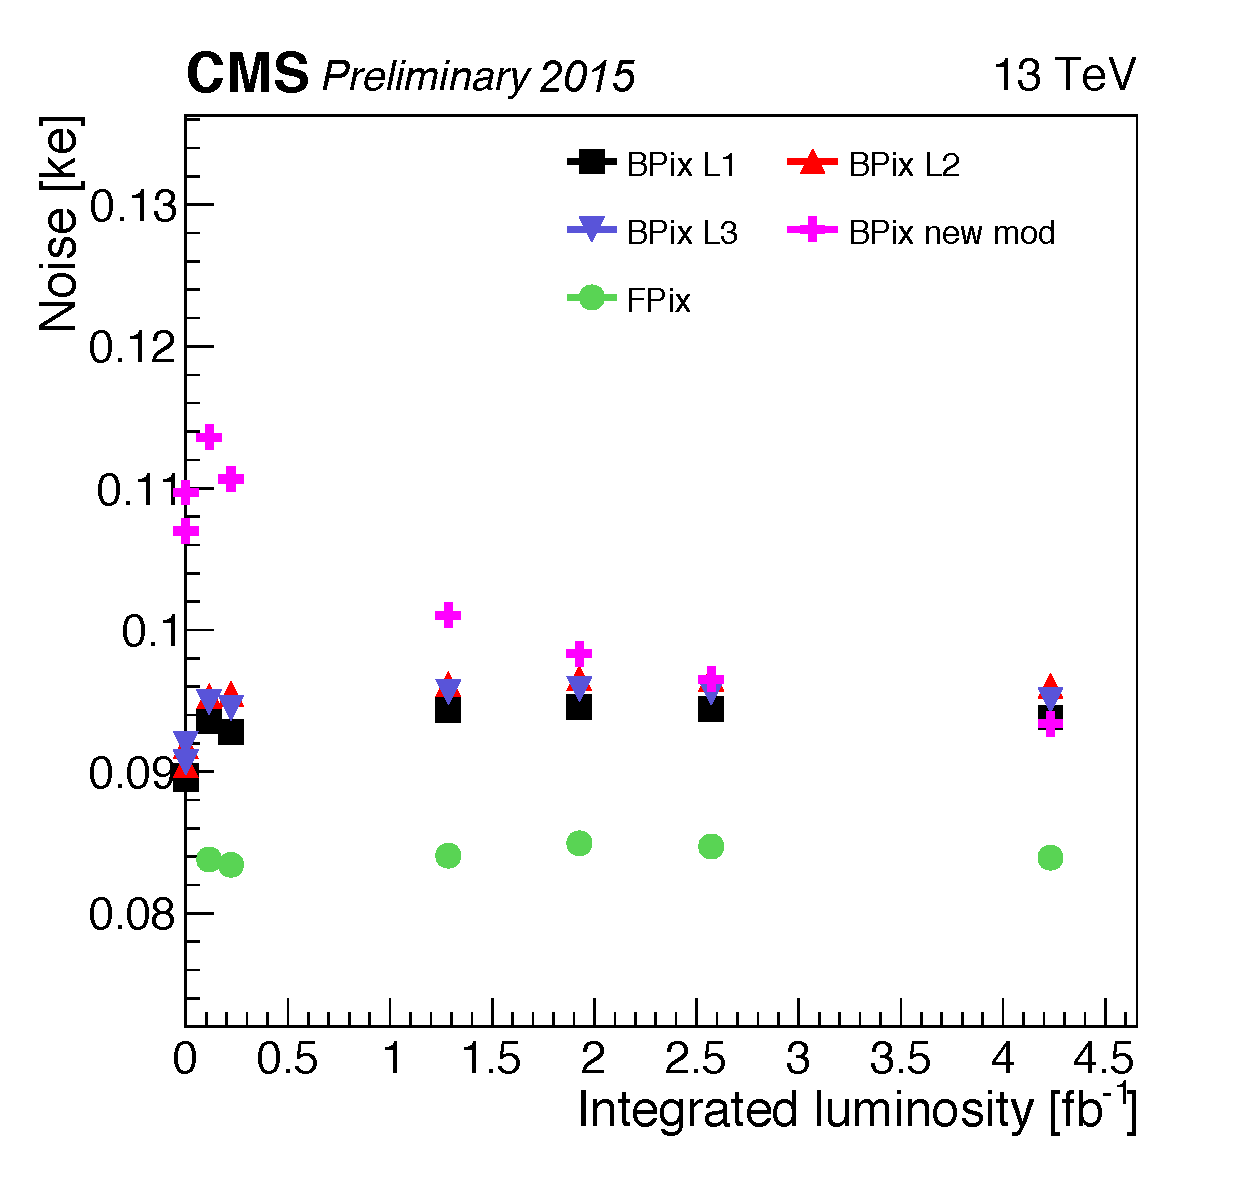
\includegraphics[width=0.3\textwidth]{\chfifteen/noisewbc2bpix_fpix.pdf}} 
 \end{center}
 \caption{Average pixel thresholds (a), RMS (b), and noise (c) measured with charge injection, using the S-curve method. The BPix modules substituted during LS1 are considered separately~\cite{PixelOffline}.}
 \label{fig:ThrVsLumi2015}
\end{figure}

\begin{figure}[!htb]
 \begin{center}
 \subfigure[]{\label{fig:ClusterChargeVsLumi_a}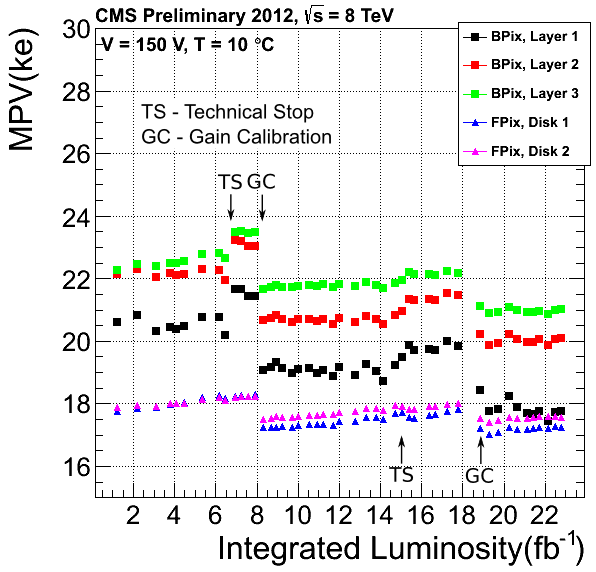
\includegraphics[width=0.3\textwidth]{\chfifteen/JLMPVwm.png}}
 \subfigure[]{\label{fig:ClusterChargeVsLumi_b}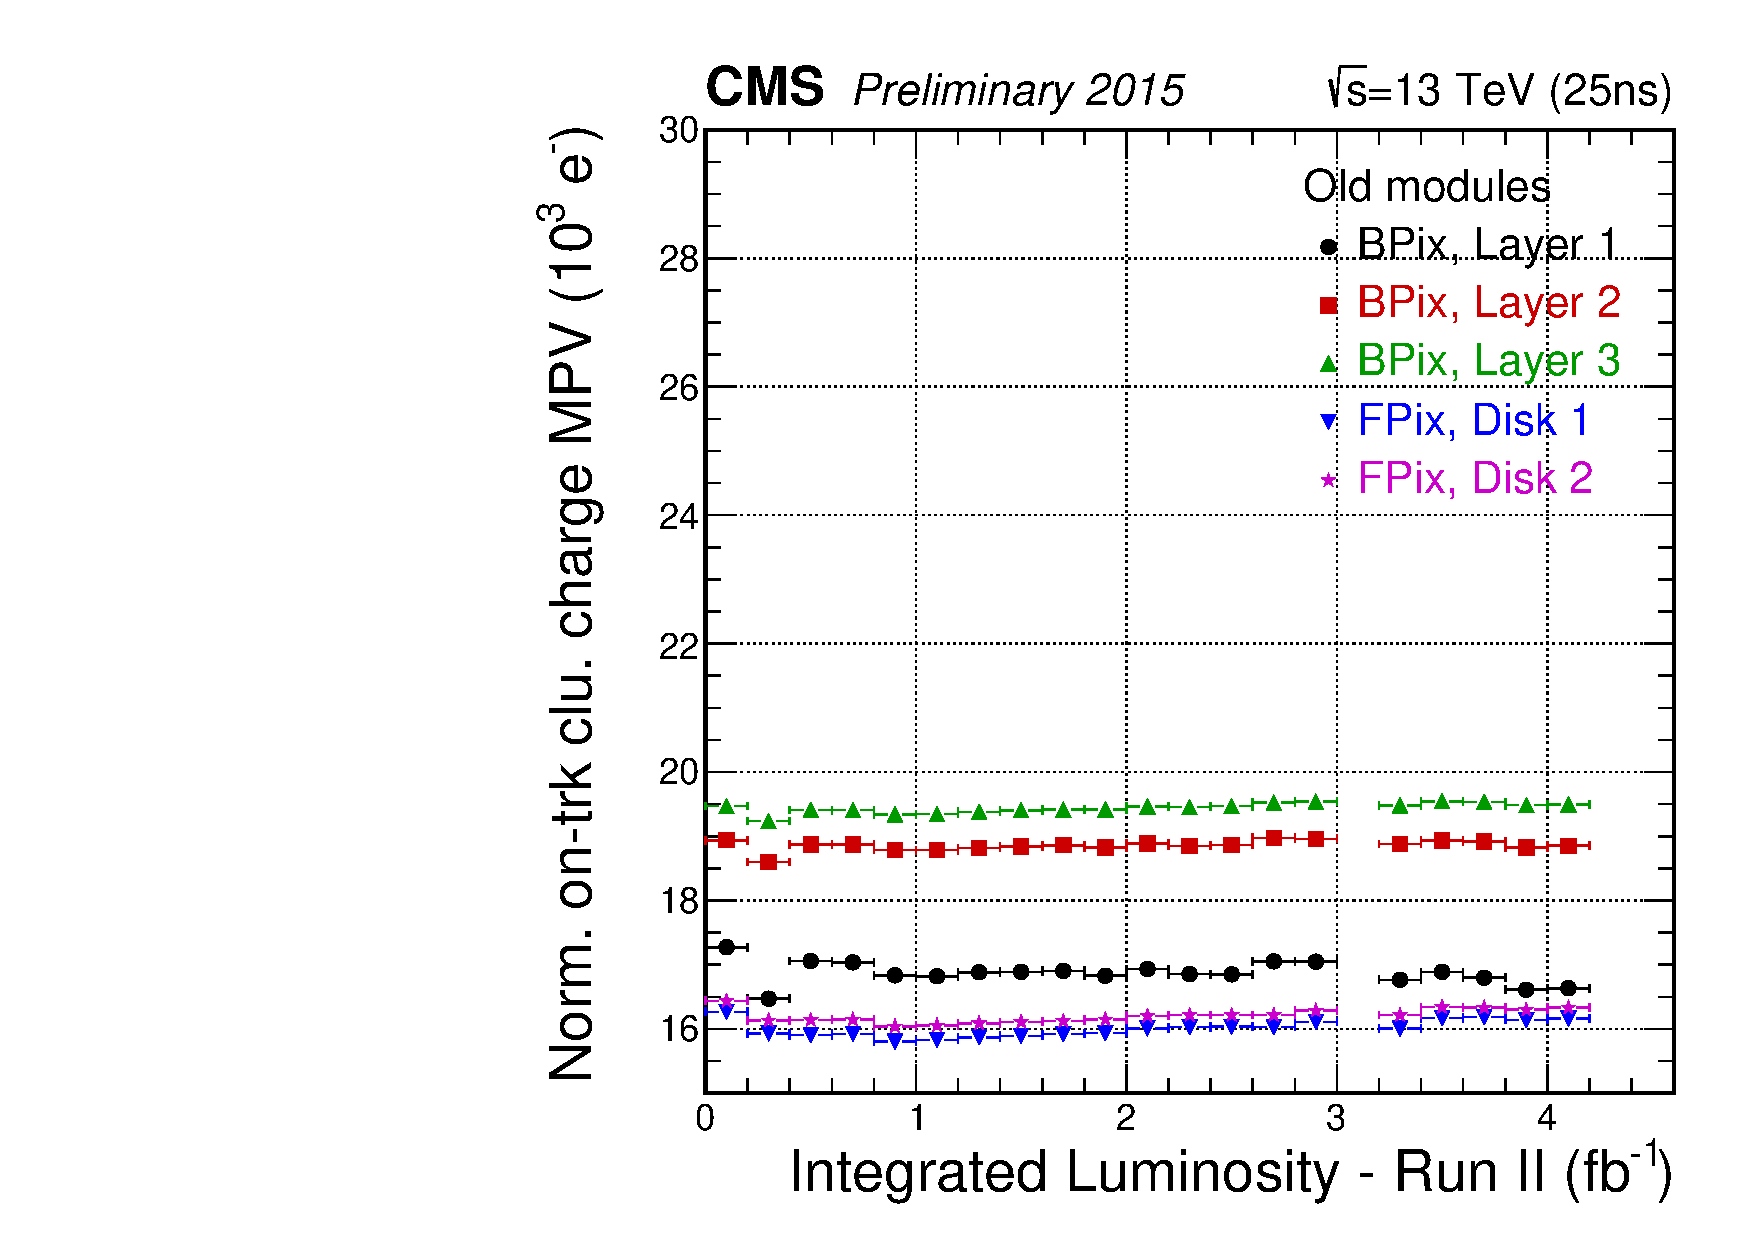
\includegraphics[width=0.3\textwidth]{\chfifteen/OnCluChargeNormMPV_vs_IntLumiRunII_LayersDisks_2015Data_OldModules.pdf}}
 \subfigure[]{\label{fig:ClusterChargeVsLumi_c}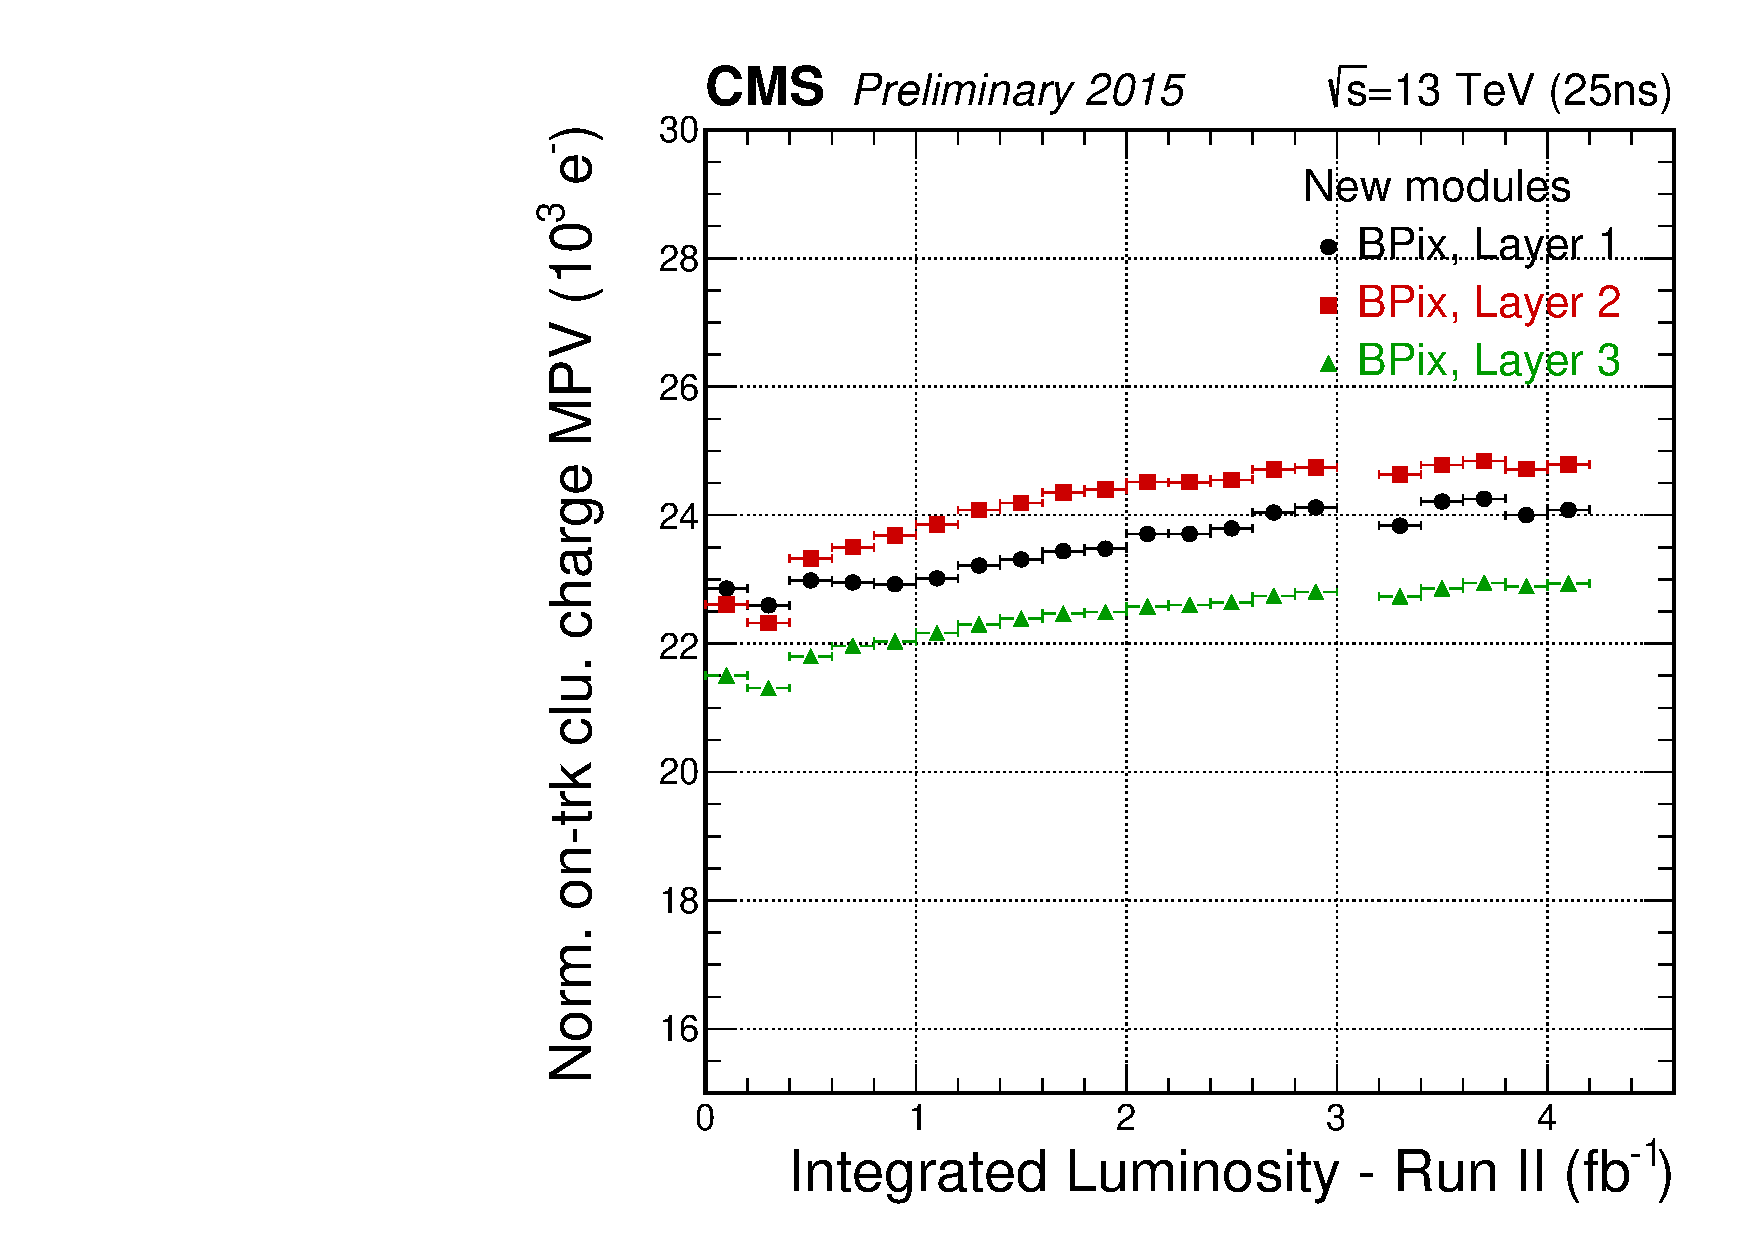
\includegraphics[width=0.3\textwidth]{\chfifteen/OnCluChargeNormMPV_vs_IntLumiRunII_LayersDisks_2015Data_NewModules.pdf}} 
 \end{center}
 \caption{The MPV of the on-track cluster charge as a function of integrated luminosity (a) in 2012, and in 2015 separately for (b) old and (c) new modules~\cite{PixelOffline}.}
 \label{fig:ClusterChargeVsLumi}
\end{figure}

Cluster properties like charge and size are important indicators of detector conditions and they have been monitored throughout the year by the pixel group.
The cluster charge is determined by fitting the Landau distribution (Fig.~\ref{fig:Landau}) arising from the hits of tracks with $\pt > 1\GeV$ and extracting the MPV parameter.
In the Run~1 measurements, the MPV changed significantly throughout the year and also after calibrations during technical stop periods (Fig.~\ref{fig:ClusterChargeVsLumi_a}).
%Each sudden increase is due to the increased cluster size after every threshold readjustment. Each sudden
%drop appears after applying a new gain calibration.  Since every threshold calibration is shown to
%restore the cluster size, the average charge should become automatically readjusted.  The overall
%negative trend, which is observed instead, may imply a change in the gain calibration
While the MPV of old modules did not change much in 2015 (Fig.~\ref{fig:ClusterChargeVsLumi_b}), the new modules showed a rapid increase (Fig.~\ref{fig:ClusterChargeVsLumi_c}).
This behavior was also observed for old modules in Run~1 in the beginning of their lifetime. No significant change in the cluster size (Fig.~\ref{fig:ClusterSizeVsLumi}) was observed.

\begin{figure}[!htb]
 \begin{center}
 \subfigure[]{\label{fig:ClusterSizeVsLumi_a}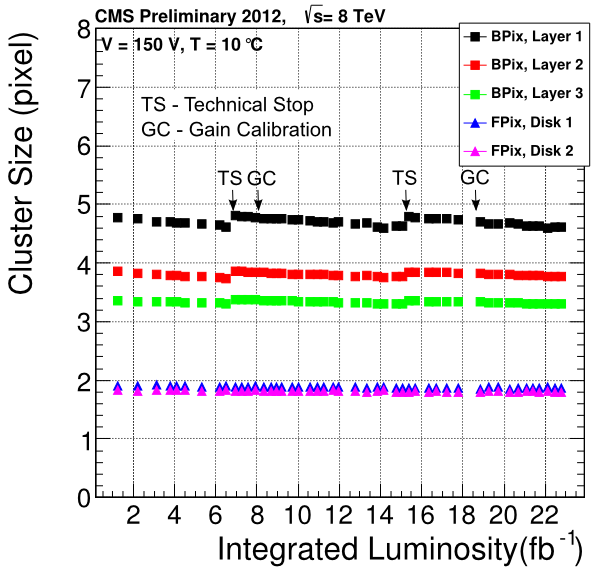
\includegraphics[width=0.4\textwidth]{\chfifteen/JLCLsize_glob.png}}
 \subfigure[]{\label{fig:ClusterSizeVsLumi_b}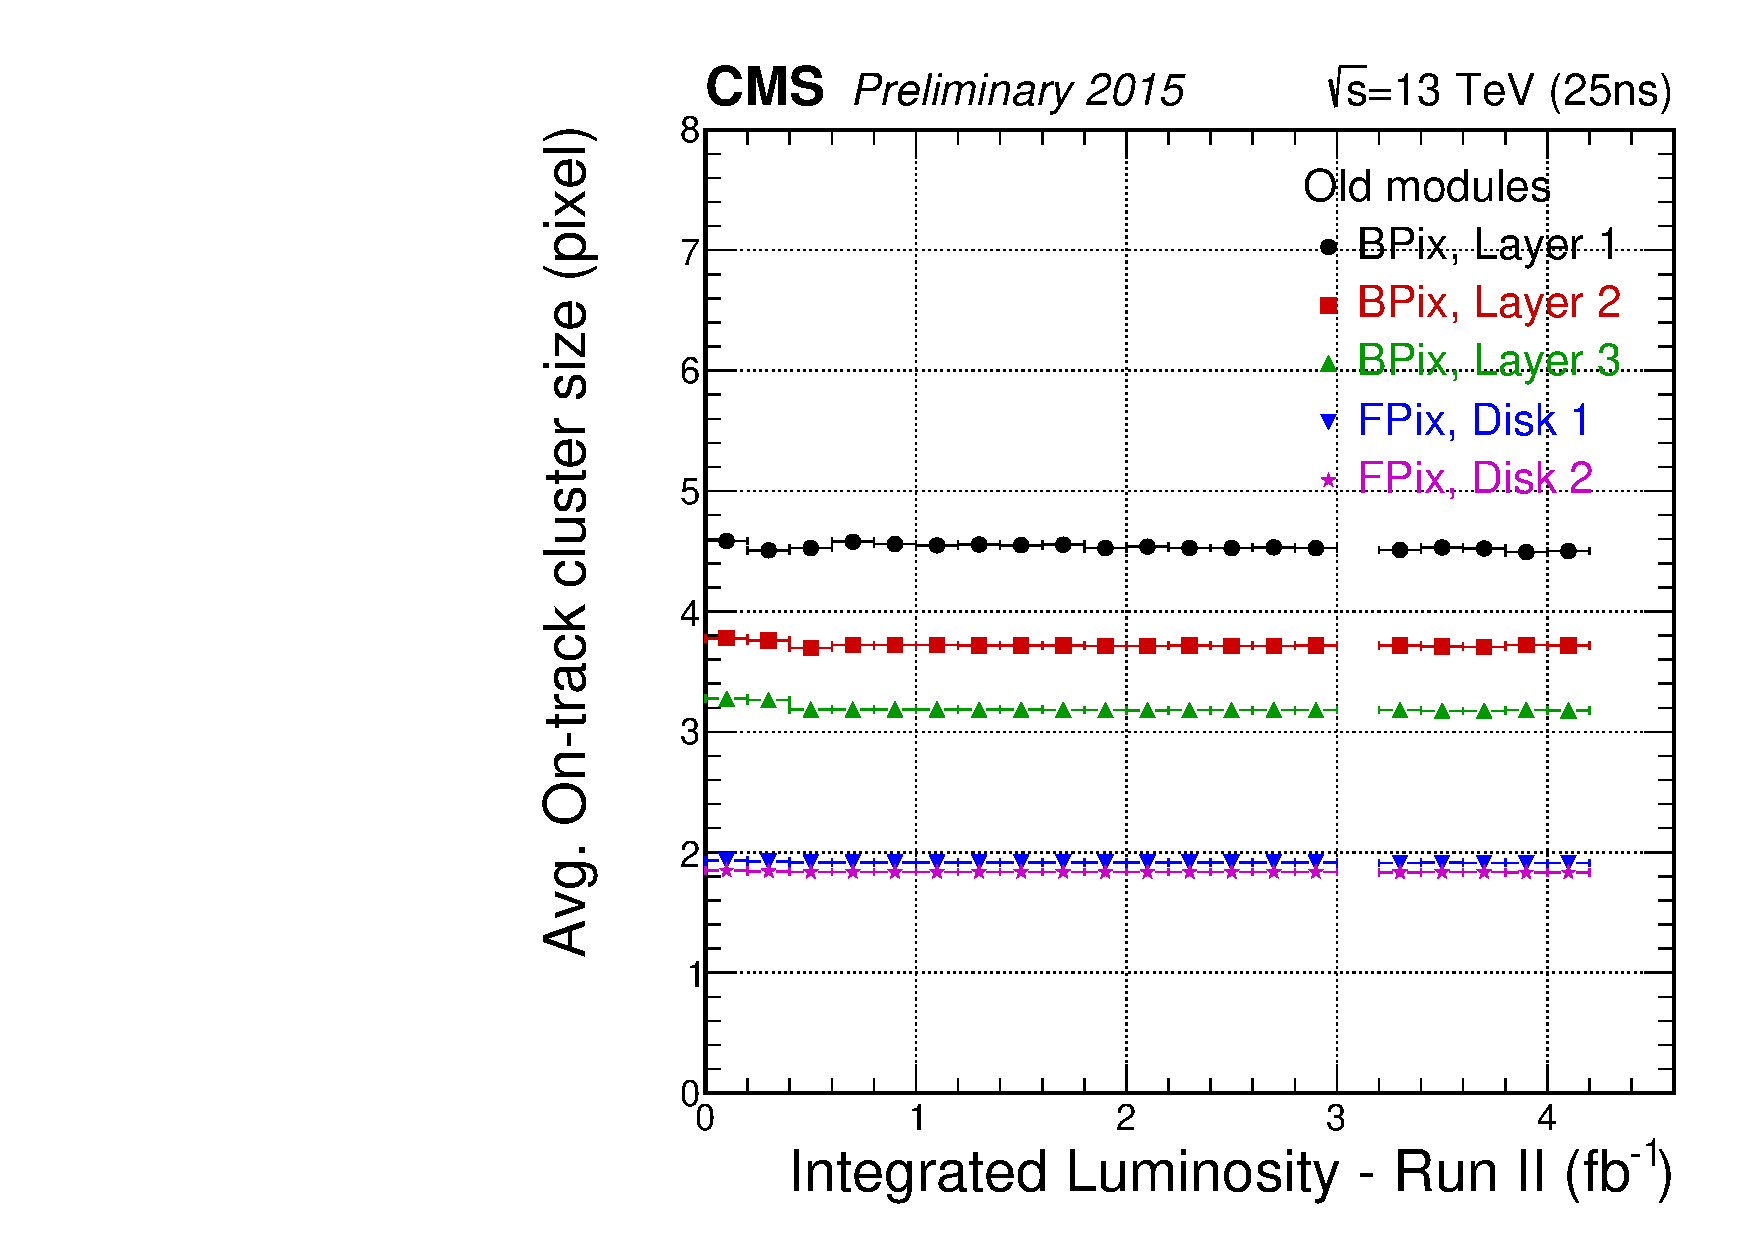
\includegraphics[width=0.4\textwidth]{\chfifteen/AvgOnCluSize_vs_IntLumiRunII_LayersDisks_2015Data_OldModules.pdf}}
 \end{center}
 \caption{Average on-track cluster size as a function of integrated luminosity in (a) Run~1 and (b) Run~2. Both old and new modules showed very similar behavior~\cite{PixelOffline}.}
 \label{fig:ClusterSizeVsLumi}
\end{figure}

Finally, the hit resolution has also been measured by the pixel group for layer 2 with tracks that have hits on layer 1 and layer 3.
The tracks are re-fitted without the hit in the middle, and the residual between the original and the interpolated hit positions are measured.
The residual distribution is then fitted with a student-t function. Figure~\ref{fig:RelVsLumi2015} shows the hit resolution as a function of the delivered luminosity in 2015.
A large improvement was observed with respect to the measurements performed at the end of Run~1 (Fig.~\ref{fig:PixRelvsLumi}).

\begin{figure}[!htb]
 \begin{center}
 \subfigure[]{\label{fig:RelVsLumi2015_a}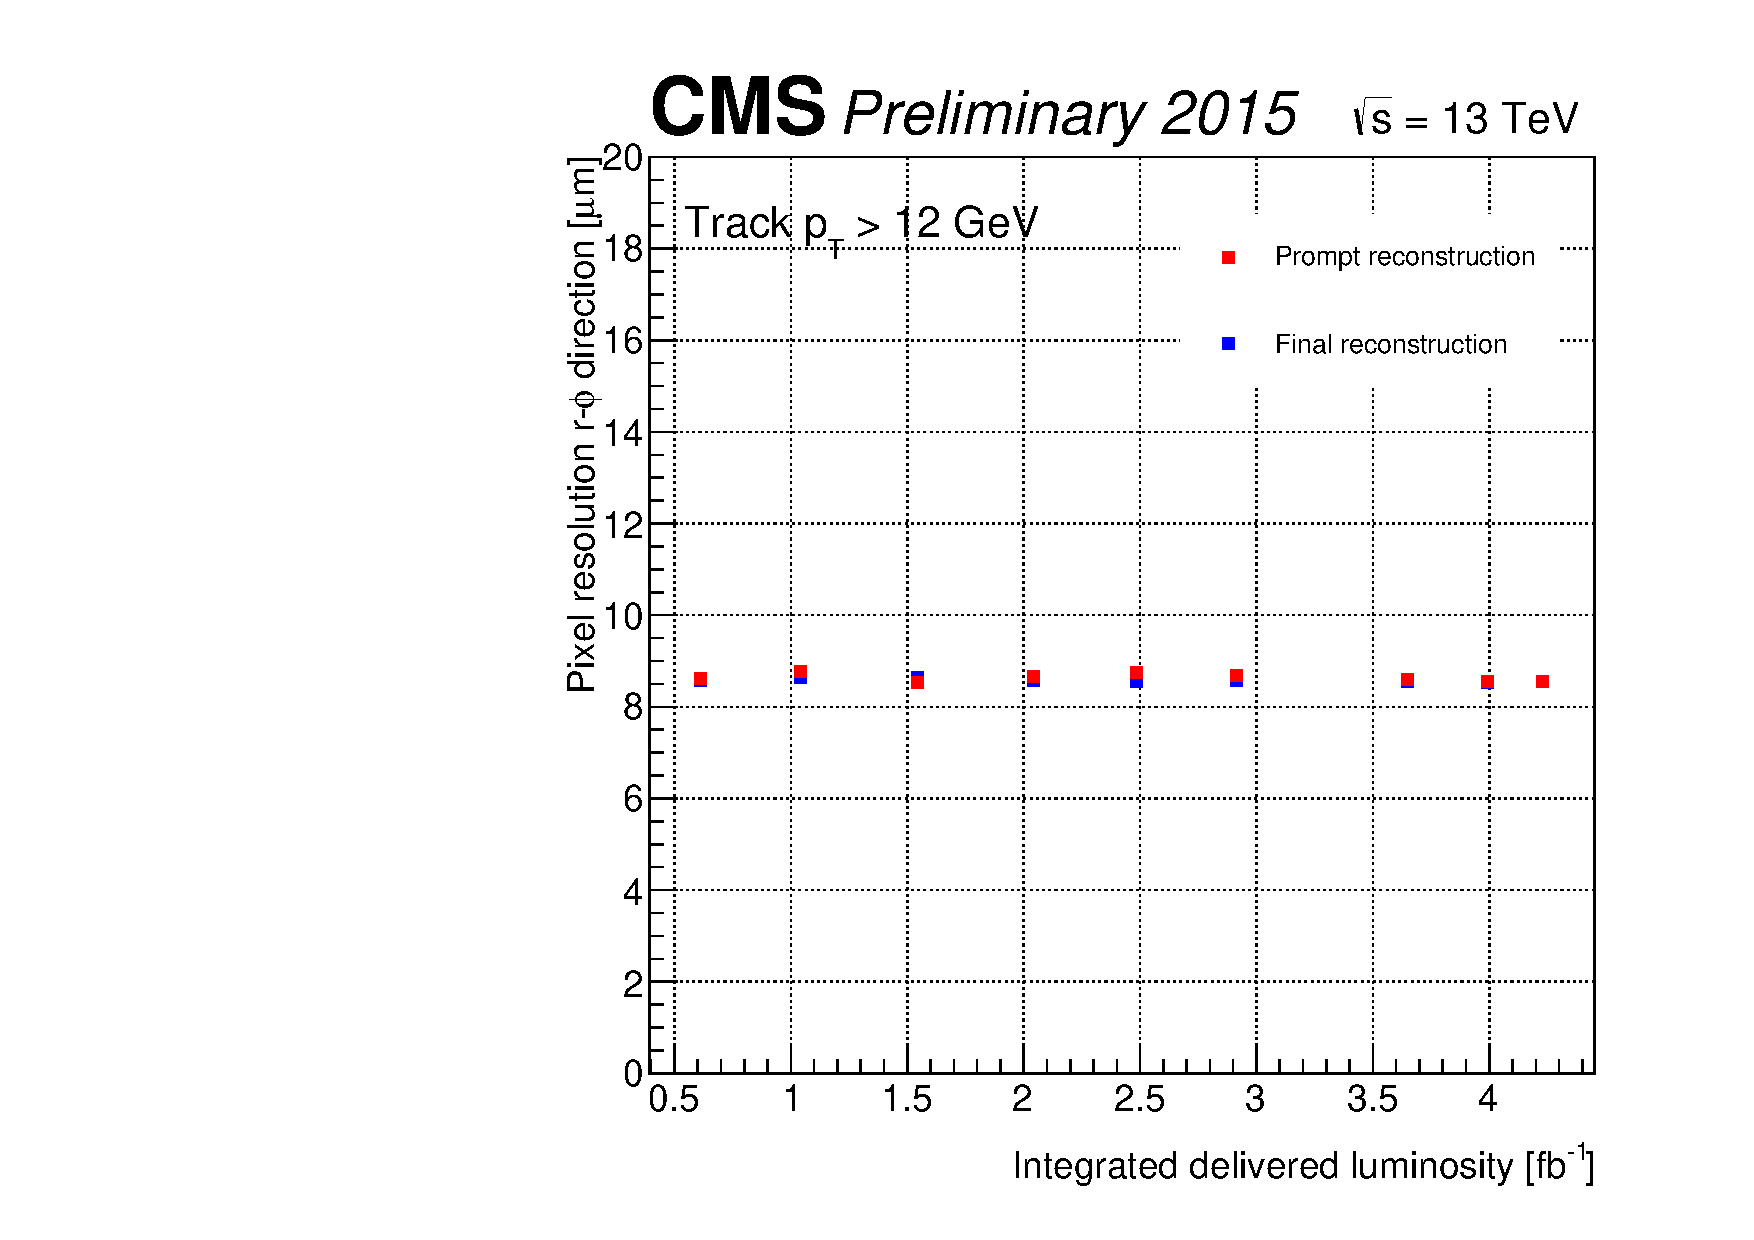
\includegraphics[width=0.4\textwidth]{\chfifteen/LumiPlot_x_Template_Prompt_ReReco_3.pdf}}
 \subfigure[]{\label{fig:RelVsLumi2015_b}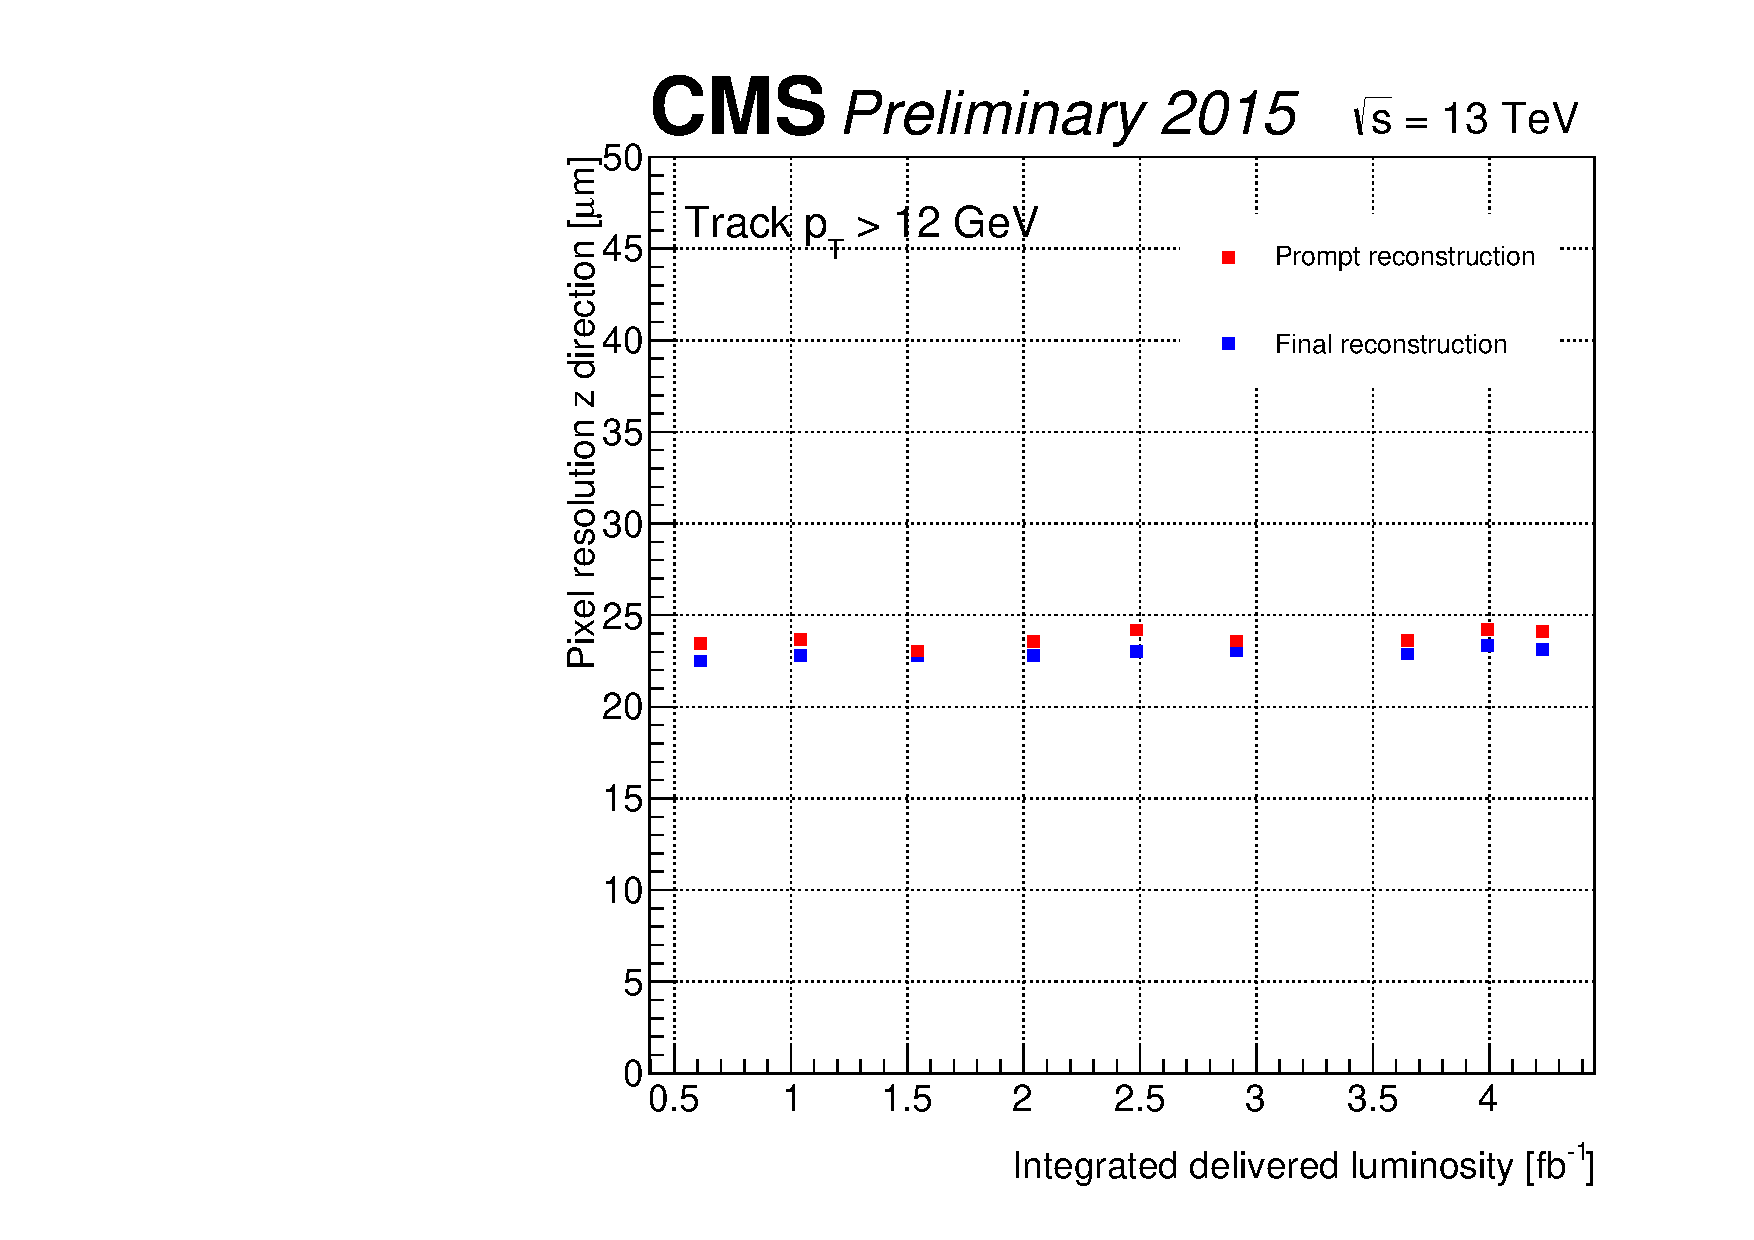
\includegraphics[width=0.4\textwidth]{\chfifteen/LumiPlot_y_Template_Prompt_ReReco_3.pdf}}
 \end{center}
 \caption{Hit resolution of barrel pixel modules in (a) the $r\phi$ and (b) the beam direction as a function of integrated luminosity in 2015~\cite{PixelOffline}.}
 \label{fig:RelVsLumi2015}
\end{figure}
